\documentclass[12pt]{article}
\usepackage[utf8]{inputenc}
\usepackage{graphicx}
\usepackage{float}
\usepackage{amsmath}
\usepackage{placeins}
\usepackage{gensymb}



\usepackage[letterpaper,margin=0.75in]{geometry}
\graphicspath{images/}
\begin{document}
\begin{titlepage}
\begin{center}
% Upper part of the page
\vbox{}
\vbox{}
\vbox{}
\vbox{}
\vbox{}
\vbox{}
\vbox{}
\vbox{}
\vbox{}
\vbox{}
\vbox{}

\includegraphics[width=0.75\textwidth]{Images/ubc.png}\\[0.5cm]
\textrm{Martin Alejo}\\[0.5cm]
\catcode`#=12
\textrm{#75296665}\\[0.5cm]
\textrm{November 18, 2022}\\[0.5cm]
\textrm{Mini Project 3}\\[0.5cm]
\textrm{University of British Columbia}\\[0.5cm]
\textrm{Electrical and Computer Engineering}\\[0.5cm]
\textrm{ELEC 301}\\[0.5cm]
\textrm{Instructor: Nicolas Jaeger}\\[0.5cm]

\includegraphics[width=0.18\textwidth]{Images/Signature.png}\\[0.5cm]
\vbox{ }
\end{center}
\end{titlepage}
\pagebreak
\pagenumbering{roman}
\tableofcontents
\pagebreak
\listoffigures
\listoftables
\pagebreak
\pagenumbering{arabic}


\section*{Introduction}
The purpose of this project is to bias and find the operating points for a cascode, and a cascade amplifier. We will also be building a differential amplifier, and AM Modulator we will be finding the bode plots. For the AM Modulator, we will be finding the saturation for an AM Modulator as well.  For this project, we will be using Multisim$^{TM}$ to simulate our circuits.

\section{Part 1 - The Cascode Amplifier}

Below is the Cascode amplifer that we need to bias: 
\begin{figure}[h!]
\centering
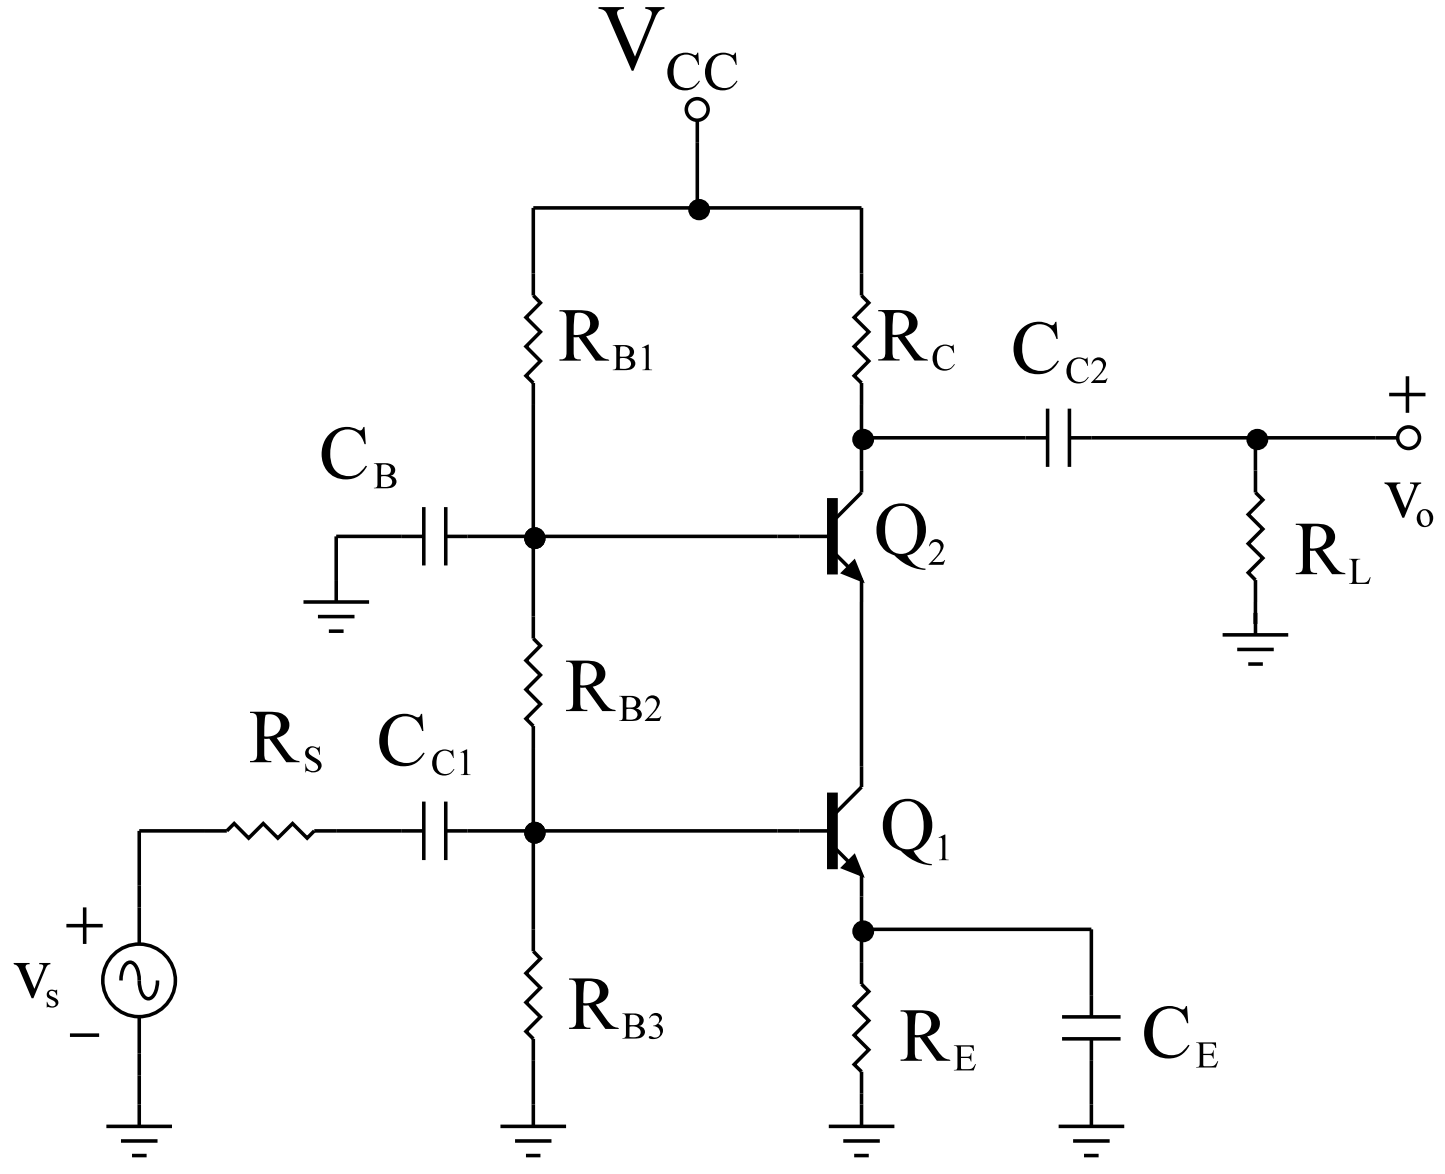
\includegraphics[height=0.25\textwidth]{Images/Part_1_circuit.png}\\
\caption{Cascode Amplifier Circuit}
\label{fig:part1_circuit}
\end{figure}

Here we will follow the amplifier specifications as according to the Project document[2]:

\begin{table}[h!]
\centering
\resizebox{\textwidth}{!}{%
\begin{tabular}{l|l|l|l}

$R_{out}$(value at mid-band) & $R_{in}$ (minimum value at mid-band) & $A_v$ (minimum value at mid-band) & $f_L$ (maximum value for low-$f$ cut-in) \\ \cline{1-4}  
2.5k$\Omega$±250$\Omega$     & 5k$\Omega$                           & 50                                  & 500Hz                                   
\end{tabular}%
}

\caption{Cascode Amplifier Specifications}
\label{table_1}
\end{table}

We will also be taking $R_S=50\Omega$, $V_{CC} = 20V$, $R_L=50k\Omega$, $C_B= 220\mu F$ and $\beta = 300$[4], from the SPICE model, according to the project document[2]. 

\subsection{Bias and $w_{3dB}$ Calculations}
Here is the circuit that we will be using the 1/4 rule on to bias the Cascode amplifier and to find the values of resistors:


\begin{figure}[h!]
\centering
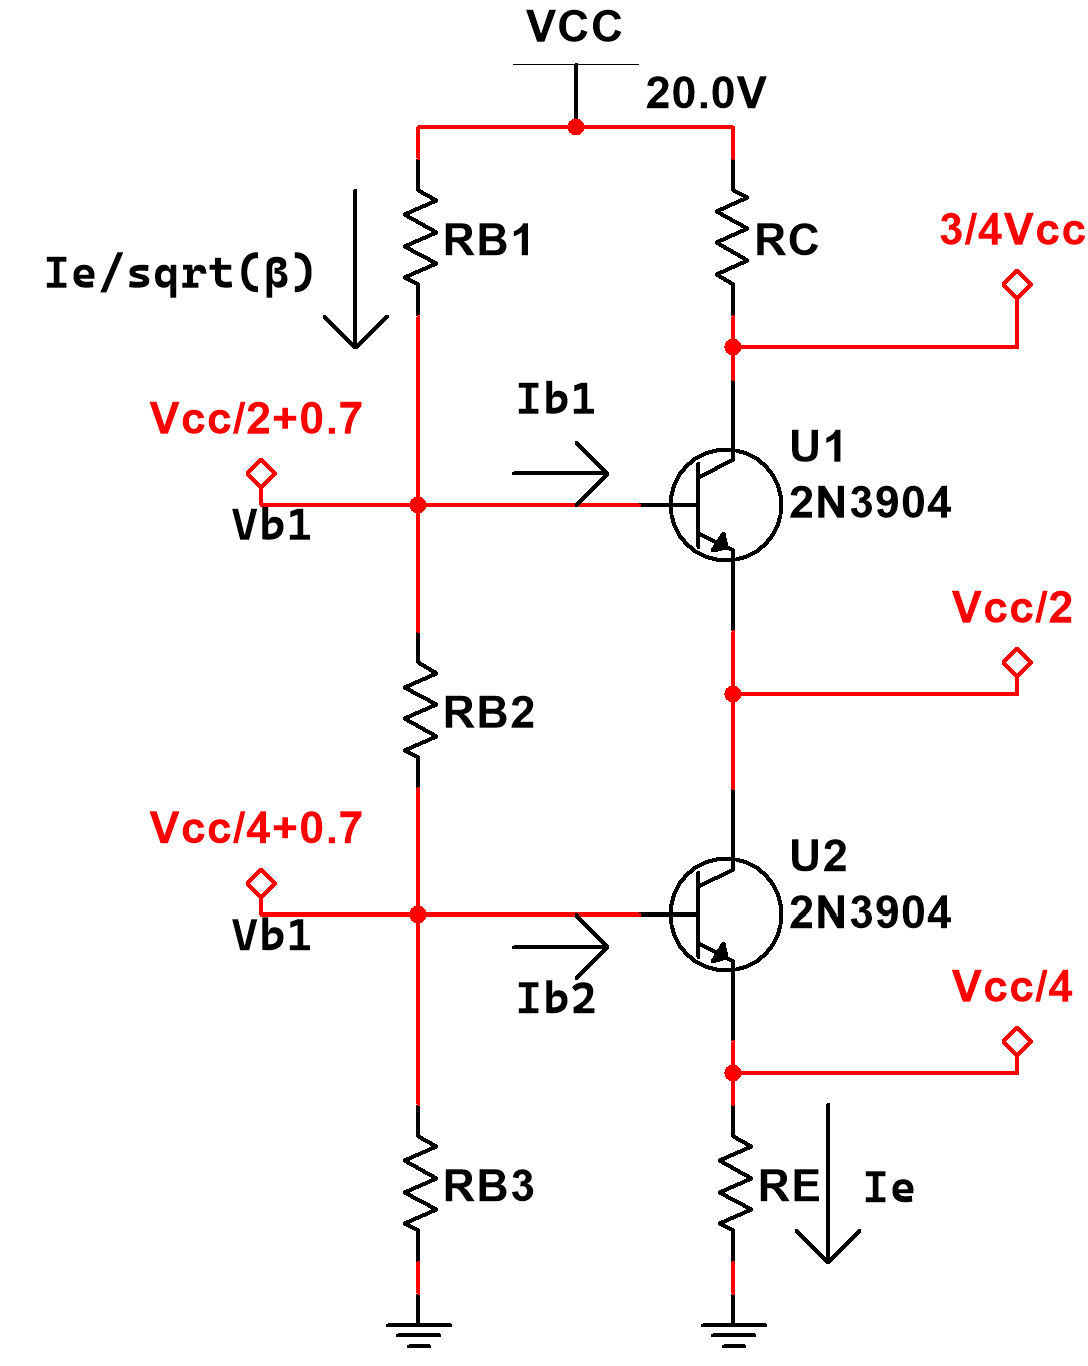
\includegraphics[height=0.30\textwidth]{Images/Part_1_biassing.png}\\
\caption{1/4 Rule Circuit}
\label{fig:part1_circuit}
\end{figure}
\FloatBarrier
We will also be biasing this circuit using standard resistances[3]. We find that $R_{out}= R_C$ so we use $R_C=2.5k\Omega$.
\newline
Using the equations from no. 1 in the appendix, we can see that:
\begin{center}
    $R_E=2.5k\Omega R_{B1}= 80.540k\Omega, R_{B2}=45.954k\Omega,R_{B3}=55.820k\Omega$.  
\end{center}
 
For the standard resistances, we can choose from the sheet[3] and find that:

\begin{center}
    $R_E$=\boxed{2.4k\Omega} $R_{B1}$= \boxed{82k\Omega}, $R_{B2}$=\boxed{47k\Omega},$R_{B3}$=\boxed{56k\Omega}.  
\end{center}

Since we know our values of the currents listed in the diagram below, we can find our small signal parameters for this circuit. The equations for which can be found in no. 2 in the appendix. The values are found to be:

\begin{table}[h!]
\centering
\begin{tabular}{l|l|l|l|l|l}
$g_{m1}$ & $g_{m2}$ & $r_{\pi1}$   & $r_{\pi2}$   & $I_{C1}$ & $I_{C2}$ \\ \cline{1-6}
0.08S    & 0.0827S  & 3750$\Omega$ & 3737$\Omega$ & 0.02A    & 0.0201A 
\end{tabular}%
\caption{Small Signal Parameters}
\label{Small Signal Model} 
\end{table}


The $R_{aux}$ resistor shown in figure \ref{fig:cascode_low_f} is so that when we calculate the input impedance, the amplifier meets the specification according to the project document[2]. The calculation to derive the value of the input can be seen from the mid-band circuit of the small signal model. The equation for which is normally $R_{in}= R_{B2}||R_{B3}||r_{\pi}$. The calculation for finding $R_{aux}$ is as shown:

\begin{center}
$5000\Omega < R_{aux}+R_{B2}||R_{B3}||r_{\pi}$
\end{center}
From here we can solve for $R_{aux}$, where it can satisfy the equation. Since we need to use standard resistors, we will set $R_{aux}$ = \boxed{3k\Omega}, which meets our amplifier specification.

For the sake of simplicity, we can just take $r_{\pi2}$=$r_{\pi1}$ and $g_{m2}$ = $g_{m1}$, since they are the same transistors.
From here we can now find our small signal model and find the value of the capacitors. Since we know our dominant low frequency pole ($f_L$), we can use that to find our value of our capacitors. We can use the following low frequency small signal model to derive our equations:


\begin{figure}[h!]
\centering
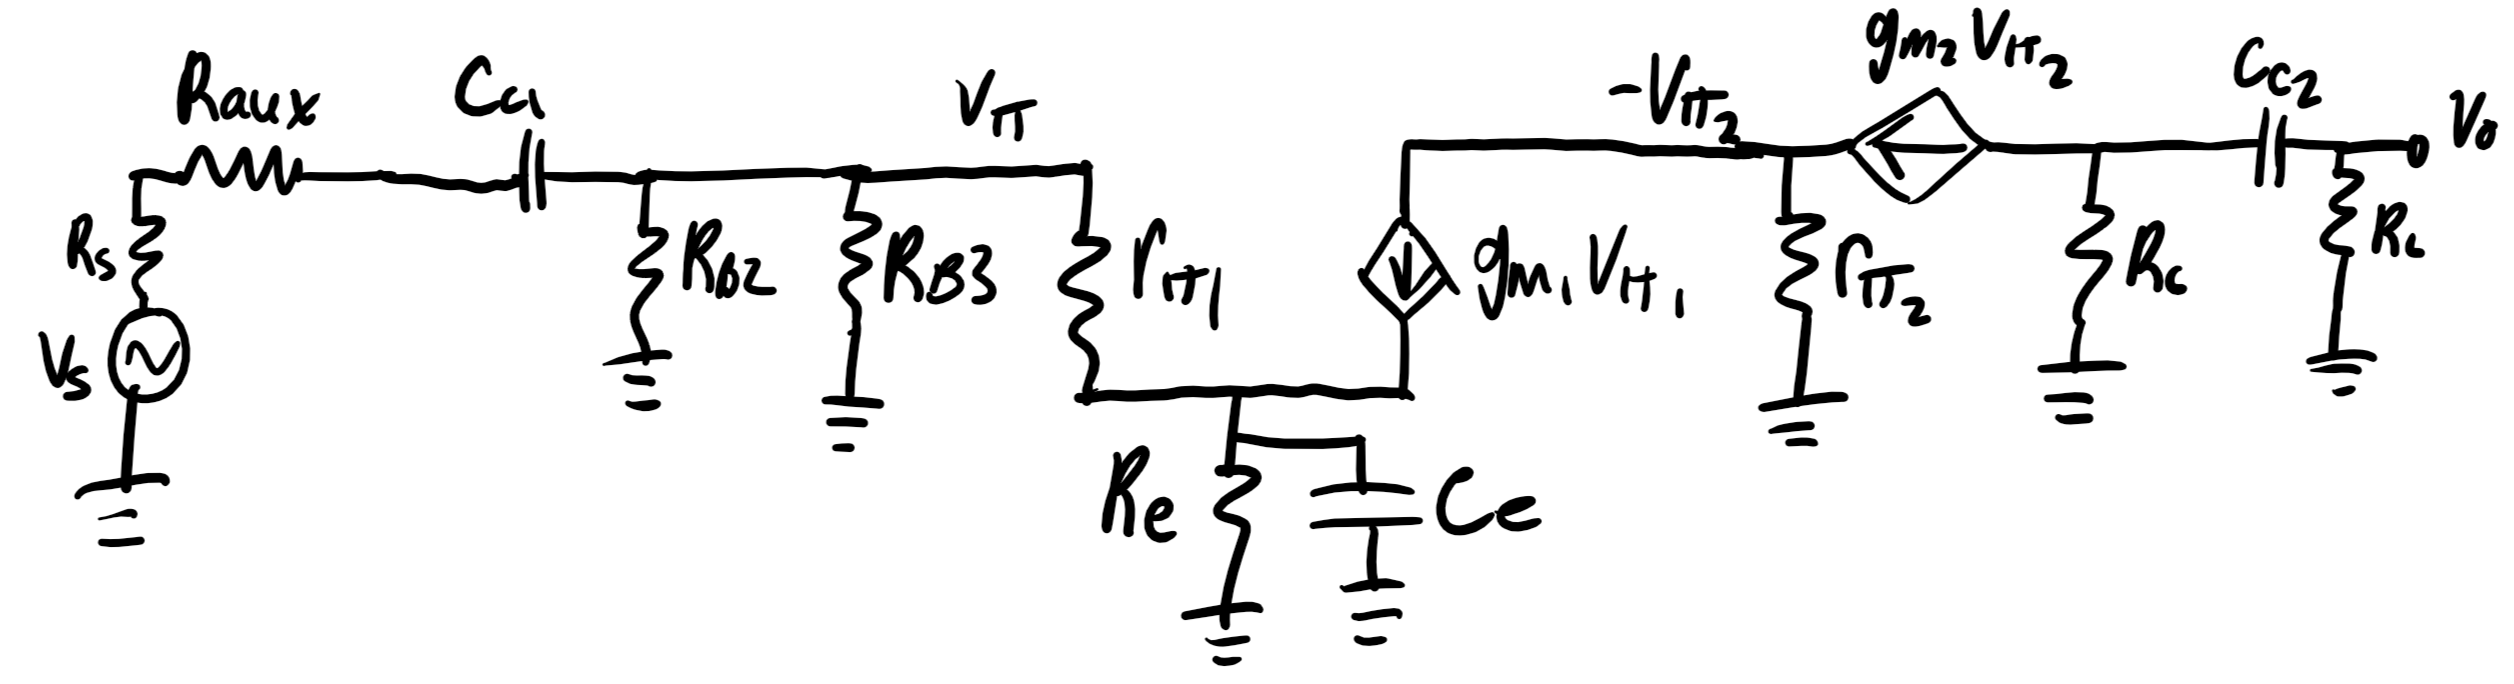
\includegraphics[height=0.15\textwidth]{Images/cascode_low_f.png}\\
\caption{Cascode Low Frequency Circuit}
\label{fig:cascode_low_f}
\end{figure}

For the sake of cost efficiency, we can determine that capacitor $C_{C1}$ shorts first. Therefore we can use the open circuit time constant equation for $C_{C1}$ and short circuit time constant equation for ${C_E}$. To determine which one is the dominant pole, we find the one that evaluates to a higher frequency. From there, we can use our given $f_L$ to find the value of the capacitor.
We can evaluate these equations to be:

\begin{flalign}
&\tau_{OC}^{C_{C1}} =C_{C1} ((R_S+R_{aux})+R_{B2}||R_{B3}||(r_{\pi1}+(1+\beta)R_E)=C_{C1}(27.735k\Omega)\nonumber)\\
&\tau_{SC}^{C_E}= C_E(R_E||(\frac{((R_S+R_{aux})||R_{B2}||R_{B3})+r_{\pi1}}{1+\beta}))=C_E(21.32\Omega)\nonumber
\end{flalign}
From the equations, we can determine that $C_E$ is the dominant pole. 
We would also know that there is a zero coupled with this pole, which can be found with $w_{LZ}=\frac{1}{R_{E}C_E}$, and we can use $w_{L3dB}=f_L*2\pi=\sqrt{(\frac{1}{\tau_{SC}^{CE}})^2-2(w_{LZ})^2}$. From here we can find $C_E$ to be \boxed{14.9\mu F}. Using the standard values, we change $C_E$ to be \boxed{22\mu F}. We will also be setting $C_{C1}$ and $C_{C2}$ to be the same value as $C_E$. 


%------------------------Part A-----------------------------------------

\subsection{Part 1 A}

Now that we have all of our values, we are  ready to measure our DC operating point using our SPICE simulation. We will use the following circuit for our simulation:

\begin{figure}[h!]
\centering
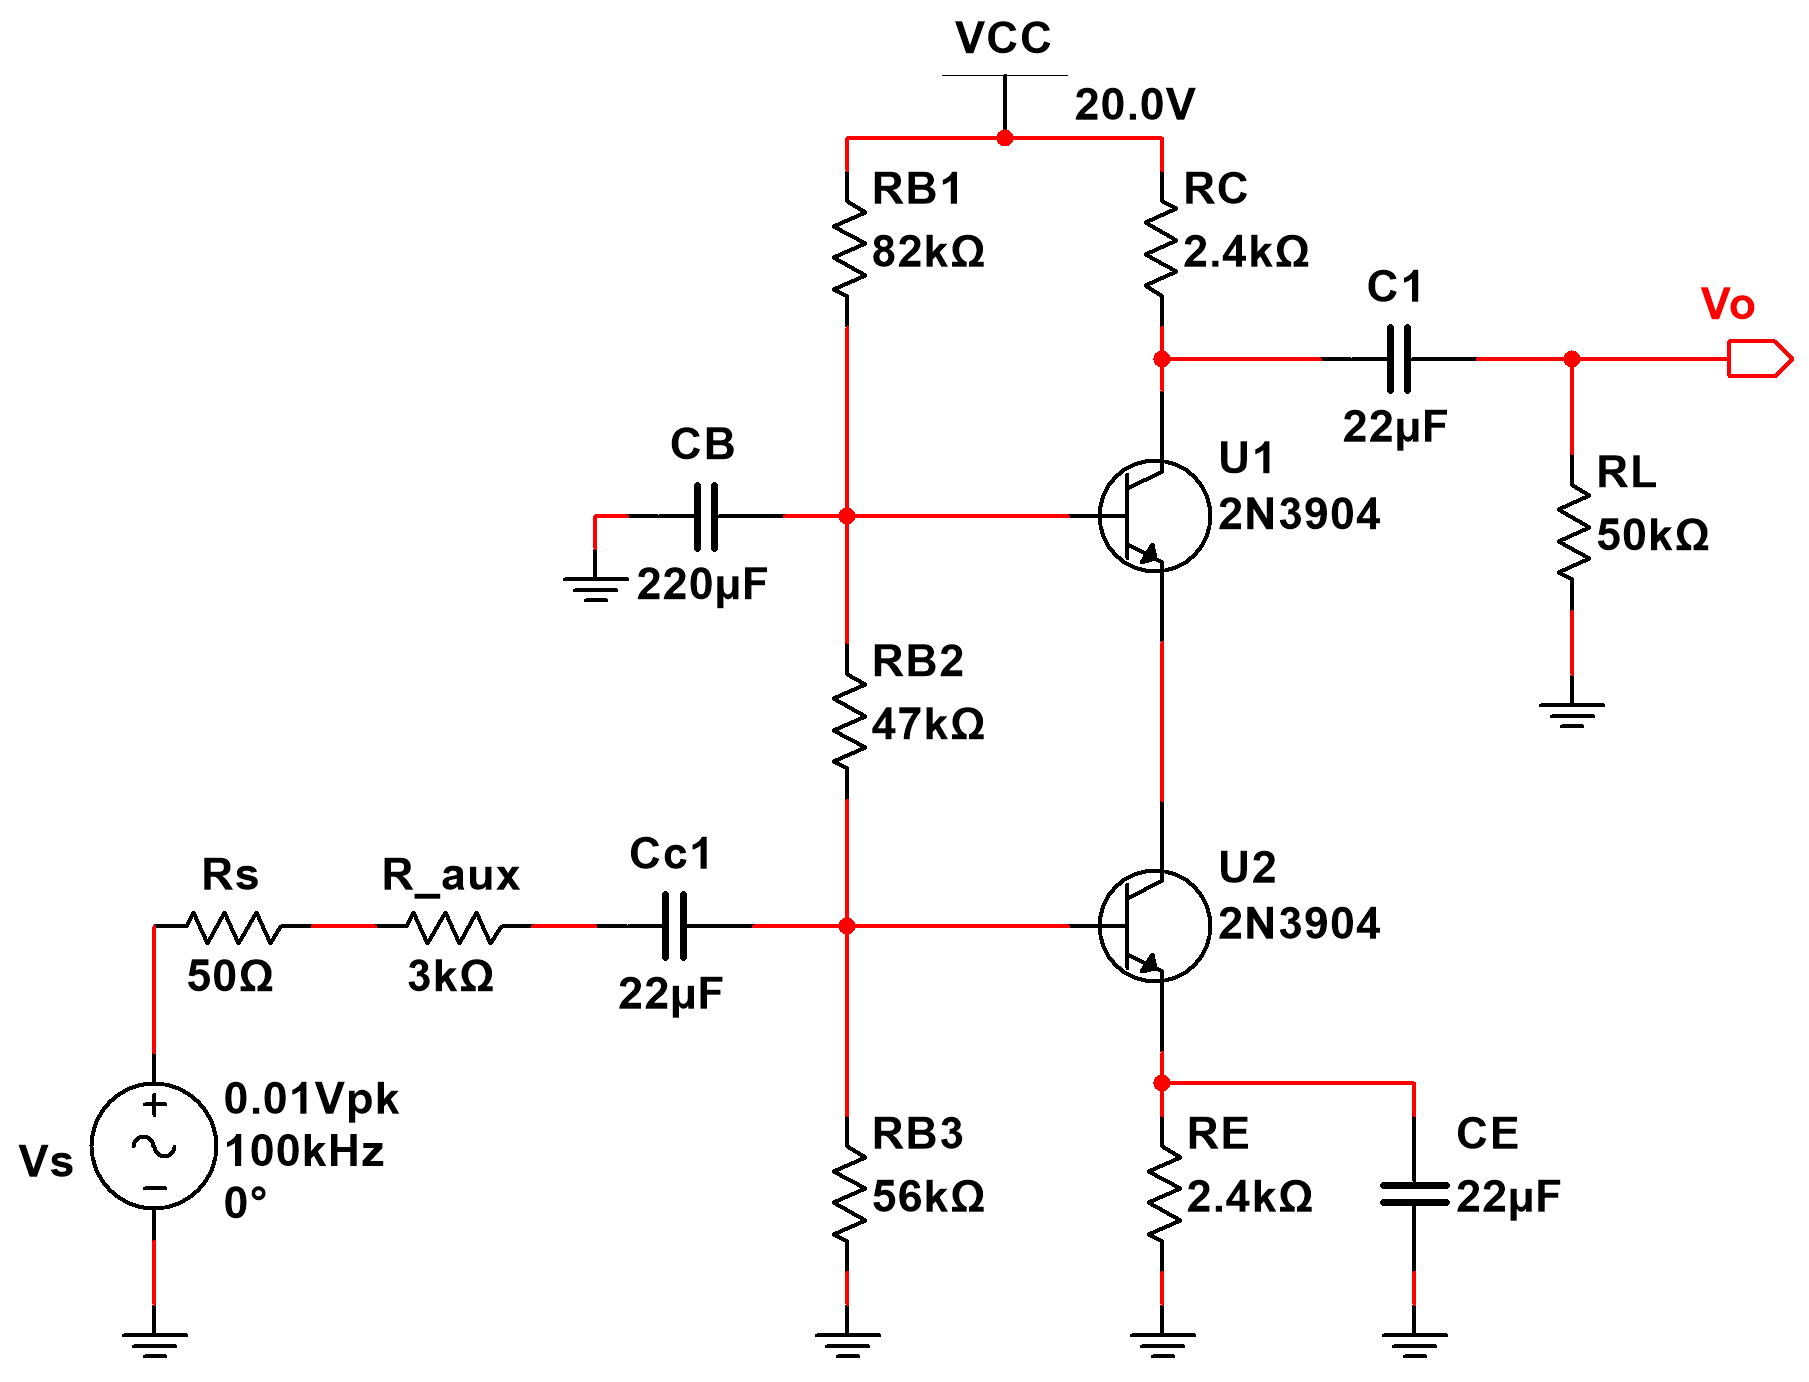
\includegraphics[height=0.30\textwidth]{Images/part_1_circuit_sim.png}\\
\caption{Cascode Amplifier Circuit}
\label{fig:part1_circuit_sim}
\end{figure}

 Here are our DC operating points:

\begin{table}[h!]
\centering
\begin{tabular}{l|llllll}
   & $I_{C}$ & $I_{B}$    & $I_{E}$ & $V_C$ & $V_B$ & $V_{E}$ \\ \cline{1-7}
U1 & 1.86mA  & 14.2$\mu$A & 1.87mA  & 15.6V  & 10.1V   & 9.48V    \\
U2 & 1.87mA  & 14.4$\mu$A & 1.89mA  & 9.48V  & 5.15V   & 4.48V   
\end{tabular}
\caption{Measured DC Operating Points}
\label{DC_op_point}
\end{table}
\FloatBarrier
\begin{table}[h!]
\centering
\begin{tabular}{l|llllll}
   & $I_{C}$ & $I_{B}$    & $I_{E}$ & $V_C$ & $V_B$ & $V_{E}$ \\ \cline{1-7}
U1 & 2.08mA  & 6.94$\mu$A & 2.09mA  & 15V  & 10.7V   & 10V    \\
U2 & 2.09mA  & 6.97$\mu$A & 2.09mA  & 10V  & 5.7V   & 5V   
\end{tabular}
\caption{Calculated DC Operating Points}
\label{DC_op_point}
\end{table}
\FloatBarrier

Comparing our DC Operating points to our calculated DC operating points, we find that they are mostly similar, aside from $I_B$ approximation, as the value is about half of the proper current. This could be due to the $\beta$ value used in the approximation, as $I_B$ calculation depended on the $\beta$ value. It seems that the $\beta$ value used in the simulation is about half the $\beta$ value used in the calculation. This could possibly mean that using the $\beta$ value as stated in the transistor SPICE model is inaccurate to the actual $\beta$ value.

\subsection{Part 1 B}
Here is the bode magnitude plot and phase for this amplifier:

\begin{figure}[h!]
\centering
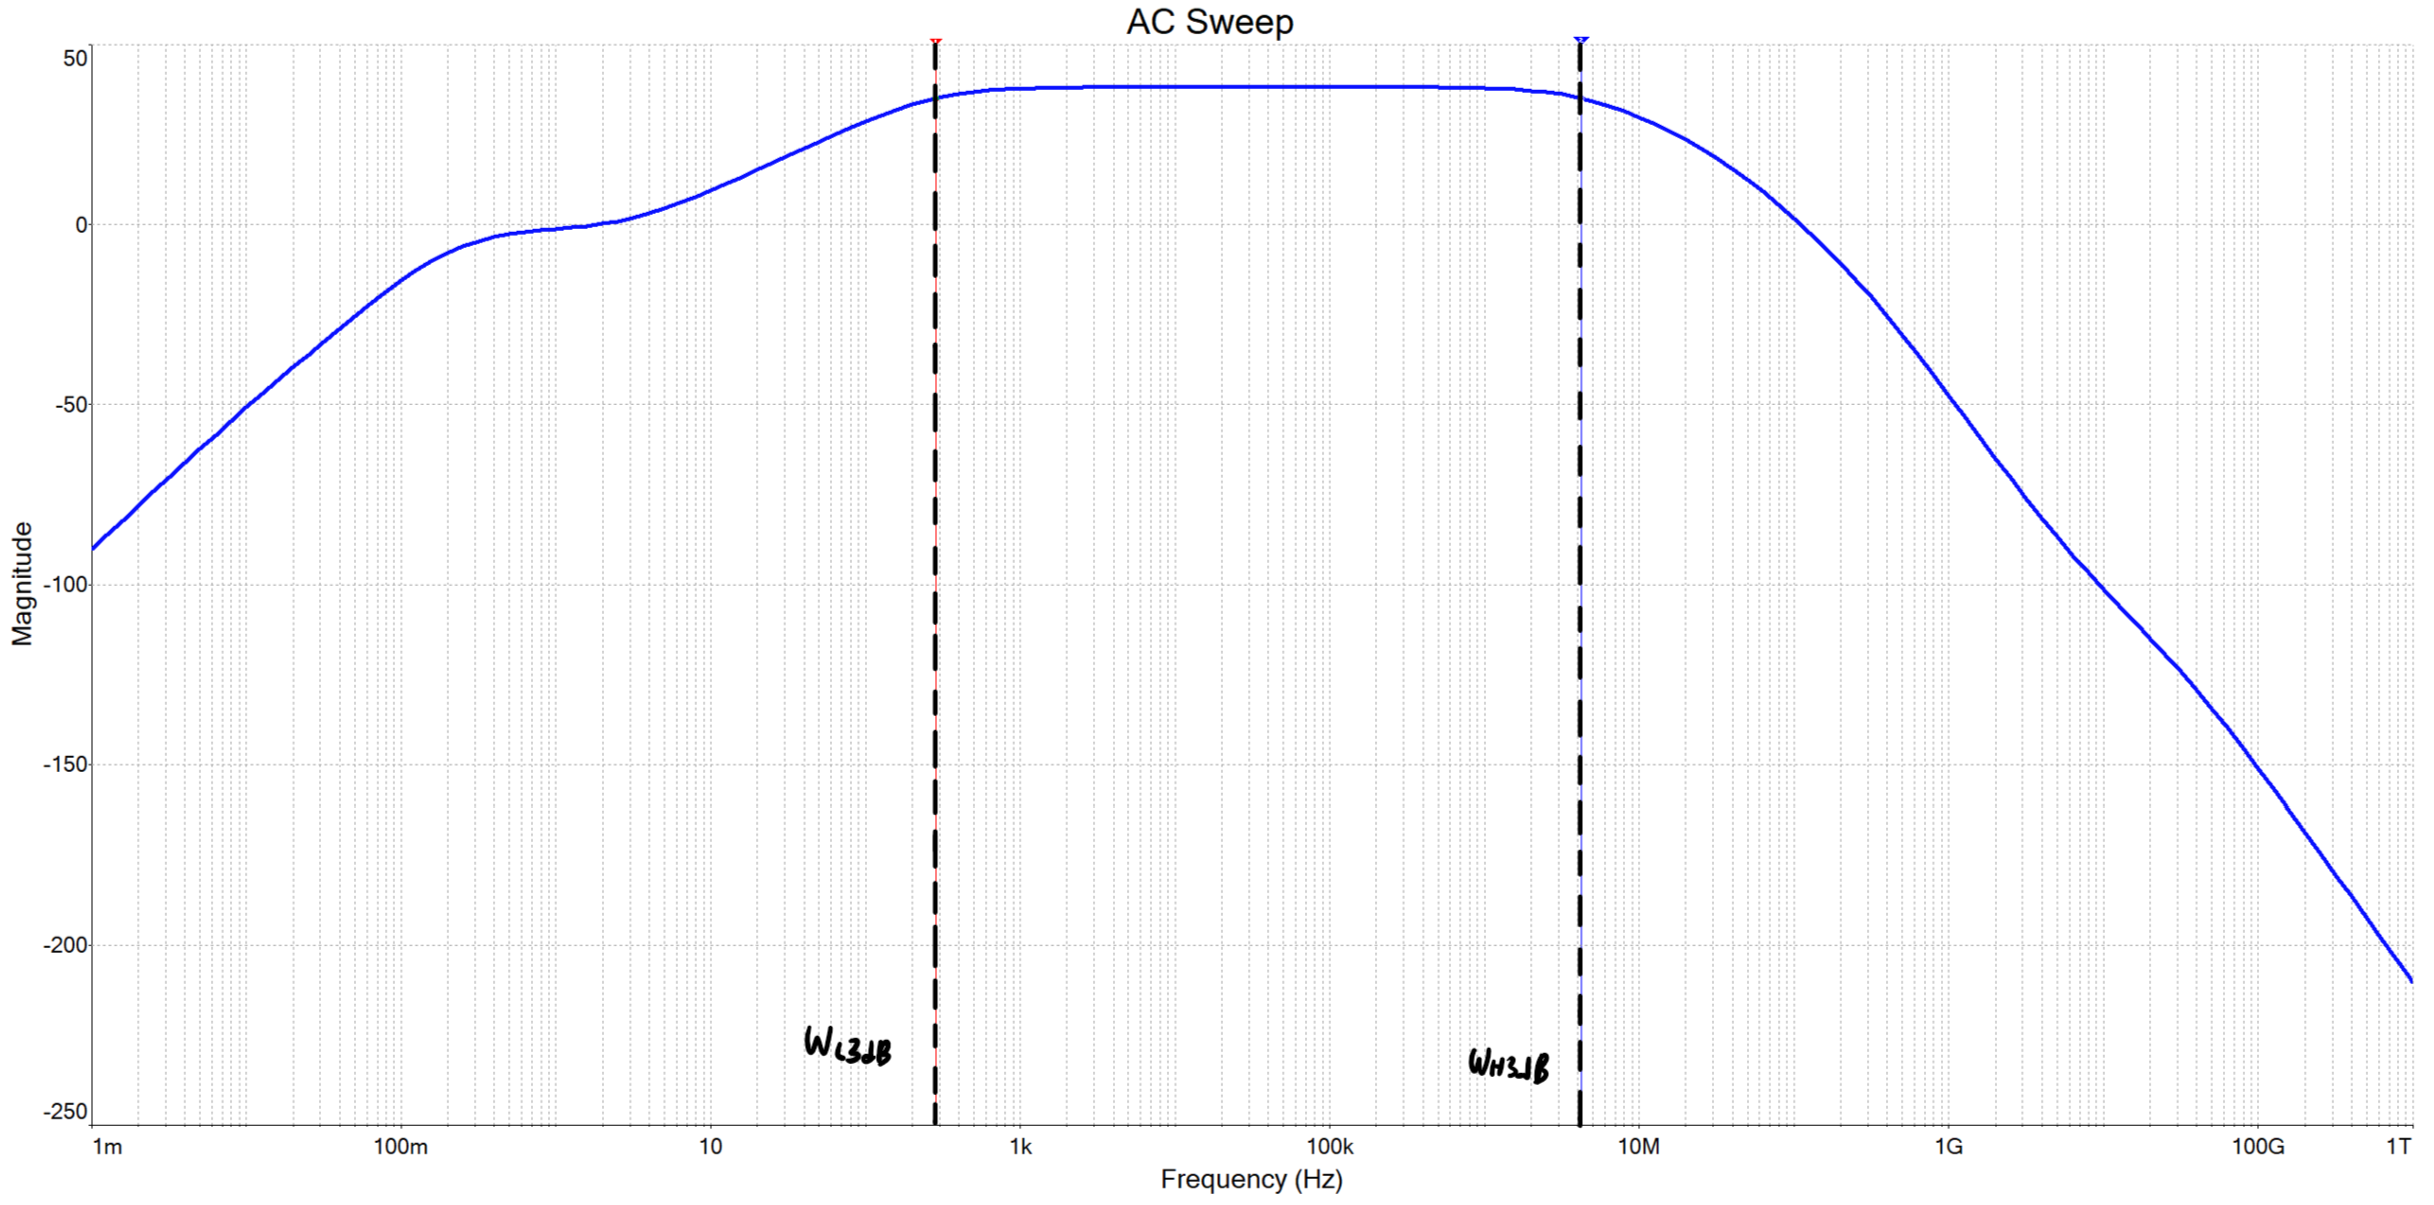
\includegraphics[height=0.35\textwidth]{Images/Part_1_magnitude.png}\\
\caption{Cascode Magnitude Plot}
\label{fig:part1_circuit_sim}
\end{figure}

\begin{figure}[h!]
\centering
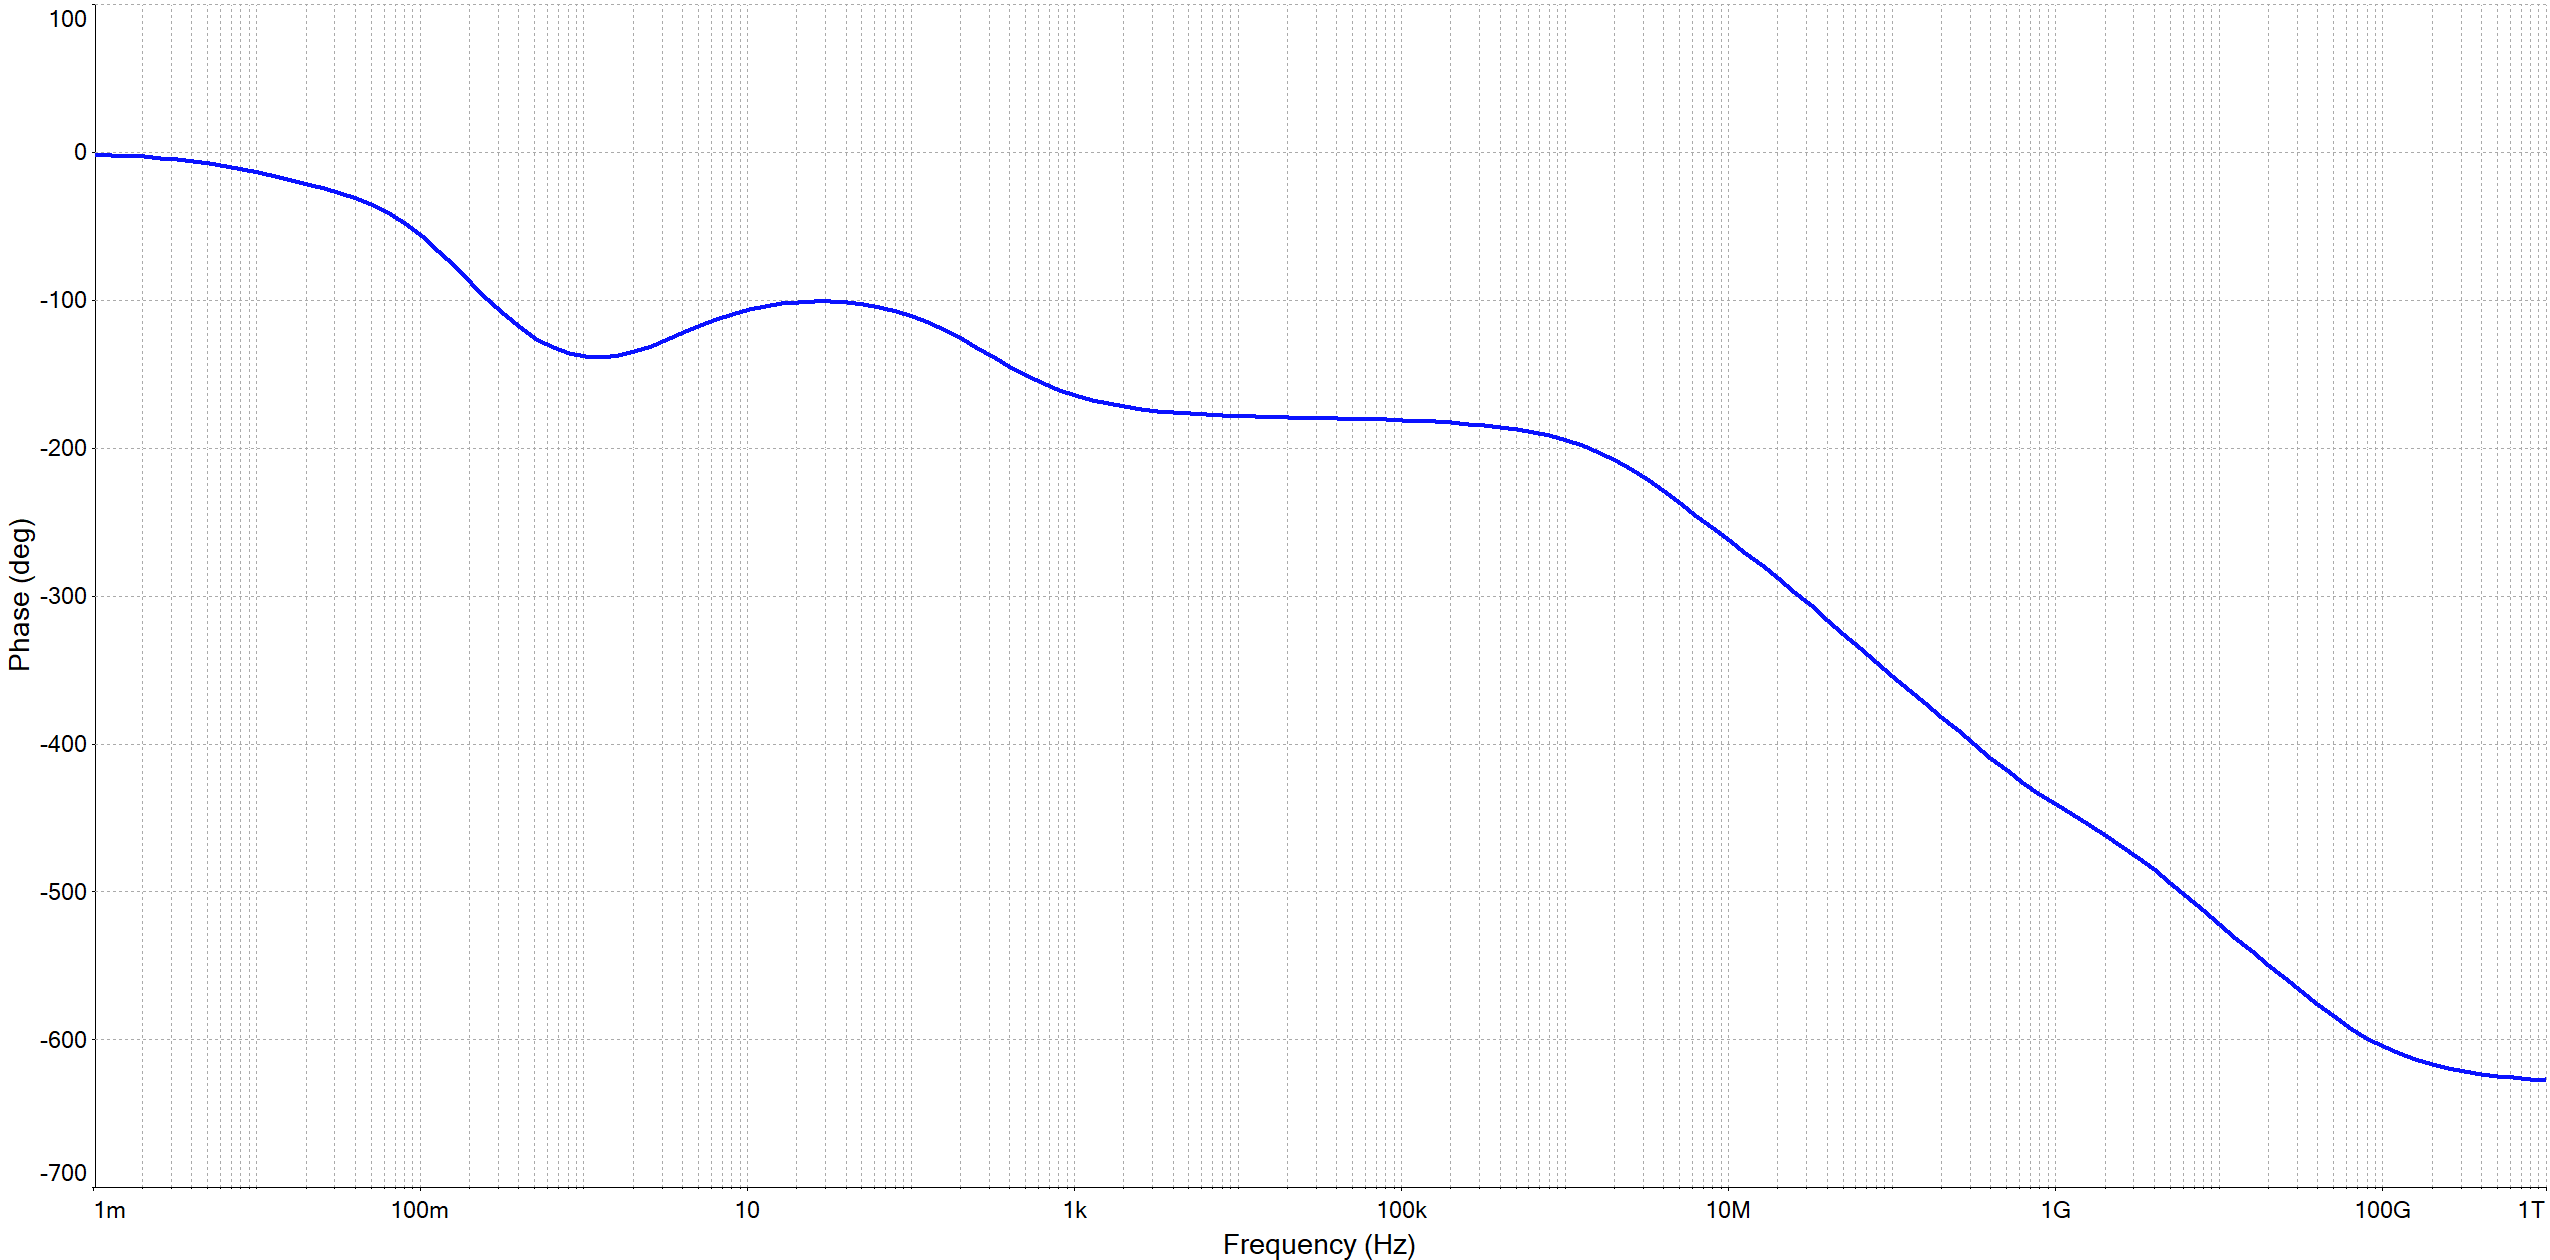
\includegraphics[height=0.35\textwidth]{Images/Part_1_phase.png}\\
\caption{Cascode Phase Plot}
\label{fig:part1_circuit_sim}
\end{figure}

The approximated $w_{L3dB}$ and $w_{H3dB}$ was evaluated to 284.576*2$\pi$ rad/s and 4.241*2$\pi*10^6$rad/s respectively.

The calculated value of each $w_{3dB}$ we can find by calculating each of the poles and zeros. The transistor parameters for $c_{\pi}$ and $c_{\mu}$ are from the SPICE model[4]. $V_{CB}$ for the $C_{\mu}$ calculations are taken from the measured DC operating points for each transistor. Since $g_m$ are the same for each transistor, we take $c_\pi$ to be the same. The calculations used to find these values are shown in no. 3 in the appendix. 

\begin{table}[]
\centering
\resizebox{\textwidth}{!}{%
\begin{tabular}{l|l|l|l|l|l|l|l|l|l|l}

 & $c_{\pi1}/c_{\pi2}$ & $c_{\mu1}$ & $c_{\mu2}$ & $w_{HP1}$ & $w_{HP2}$ & $w_{HP3}$ & $w_{LP1}$ & $w_{LP2}$ & $w_{L3dB}$ & $w_{H3dB}$ \\ \hline
Calculated Values & 41pF & 1.739pF & 1.861pF & 456.5M rad/s & 234.556 M rad/s & 1810.686 M rad/s & 1.713 rad/s & 2.518k rad/s & 2.518k rad/s & 207.261 M rad/s \\
\end{tabular}%
}
\caption{Calculated Frequencies and Capacitance}
\label{Bias Resistor and Capacitor Values}
\end{table}

The $w_{LP2}$ pole in the low 3dB calculation was doubled because the contribution of $C_{C2}$ is identical.
Comparing from the values the measured and the calculated, we can see that both the low frequency and high frequency $w_{3dB}$ estimates are not very accurate to the calculated values.

\subsection{Part 1 C}

For the mid-band frequency, we will be using 100kHz. We will be adjusting the amplitude by 0.01V until we see non-linearity in the voltage transfer curve. Below is the voltage transfer curve:

\begin{figure}[h!]
\centering
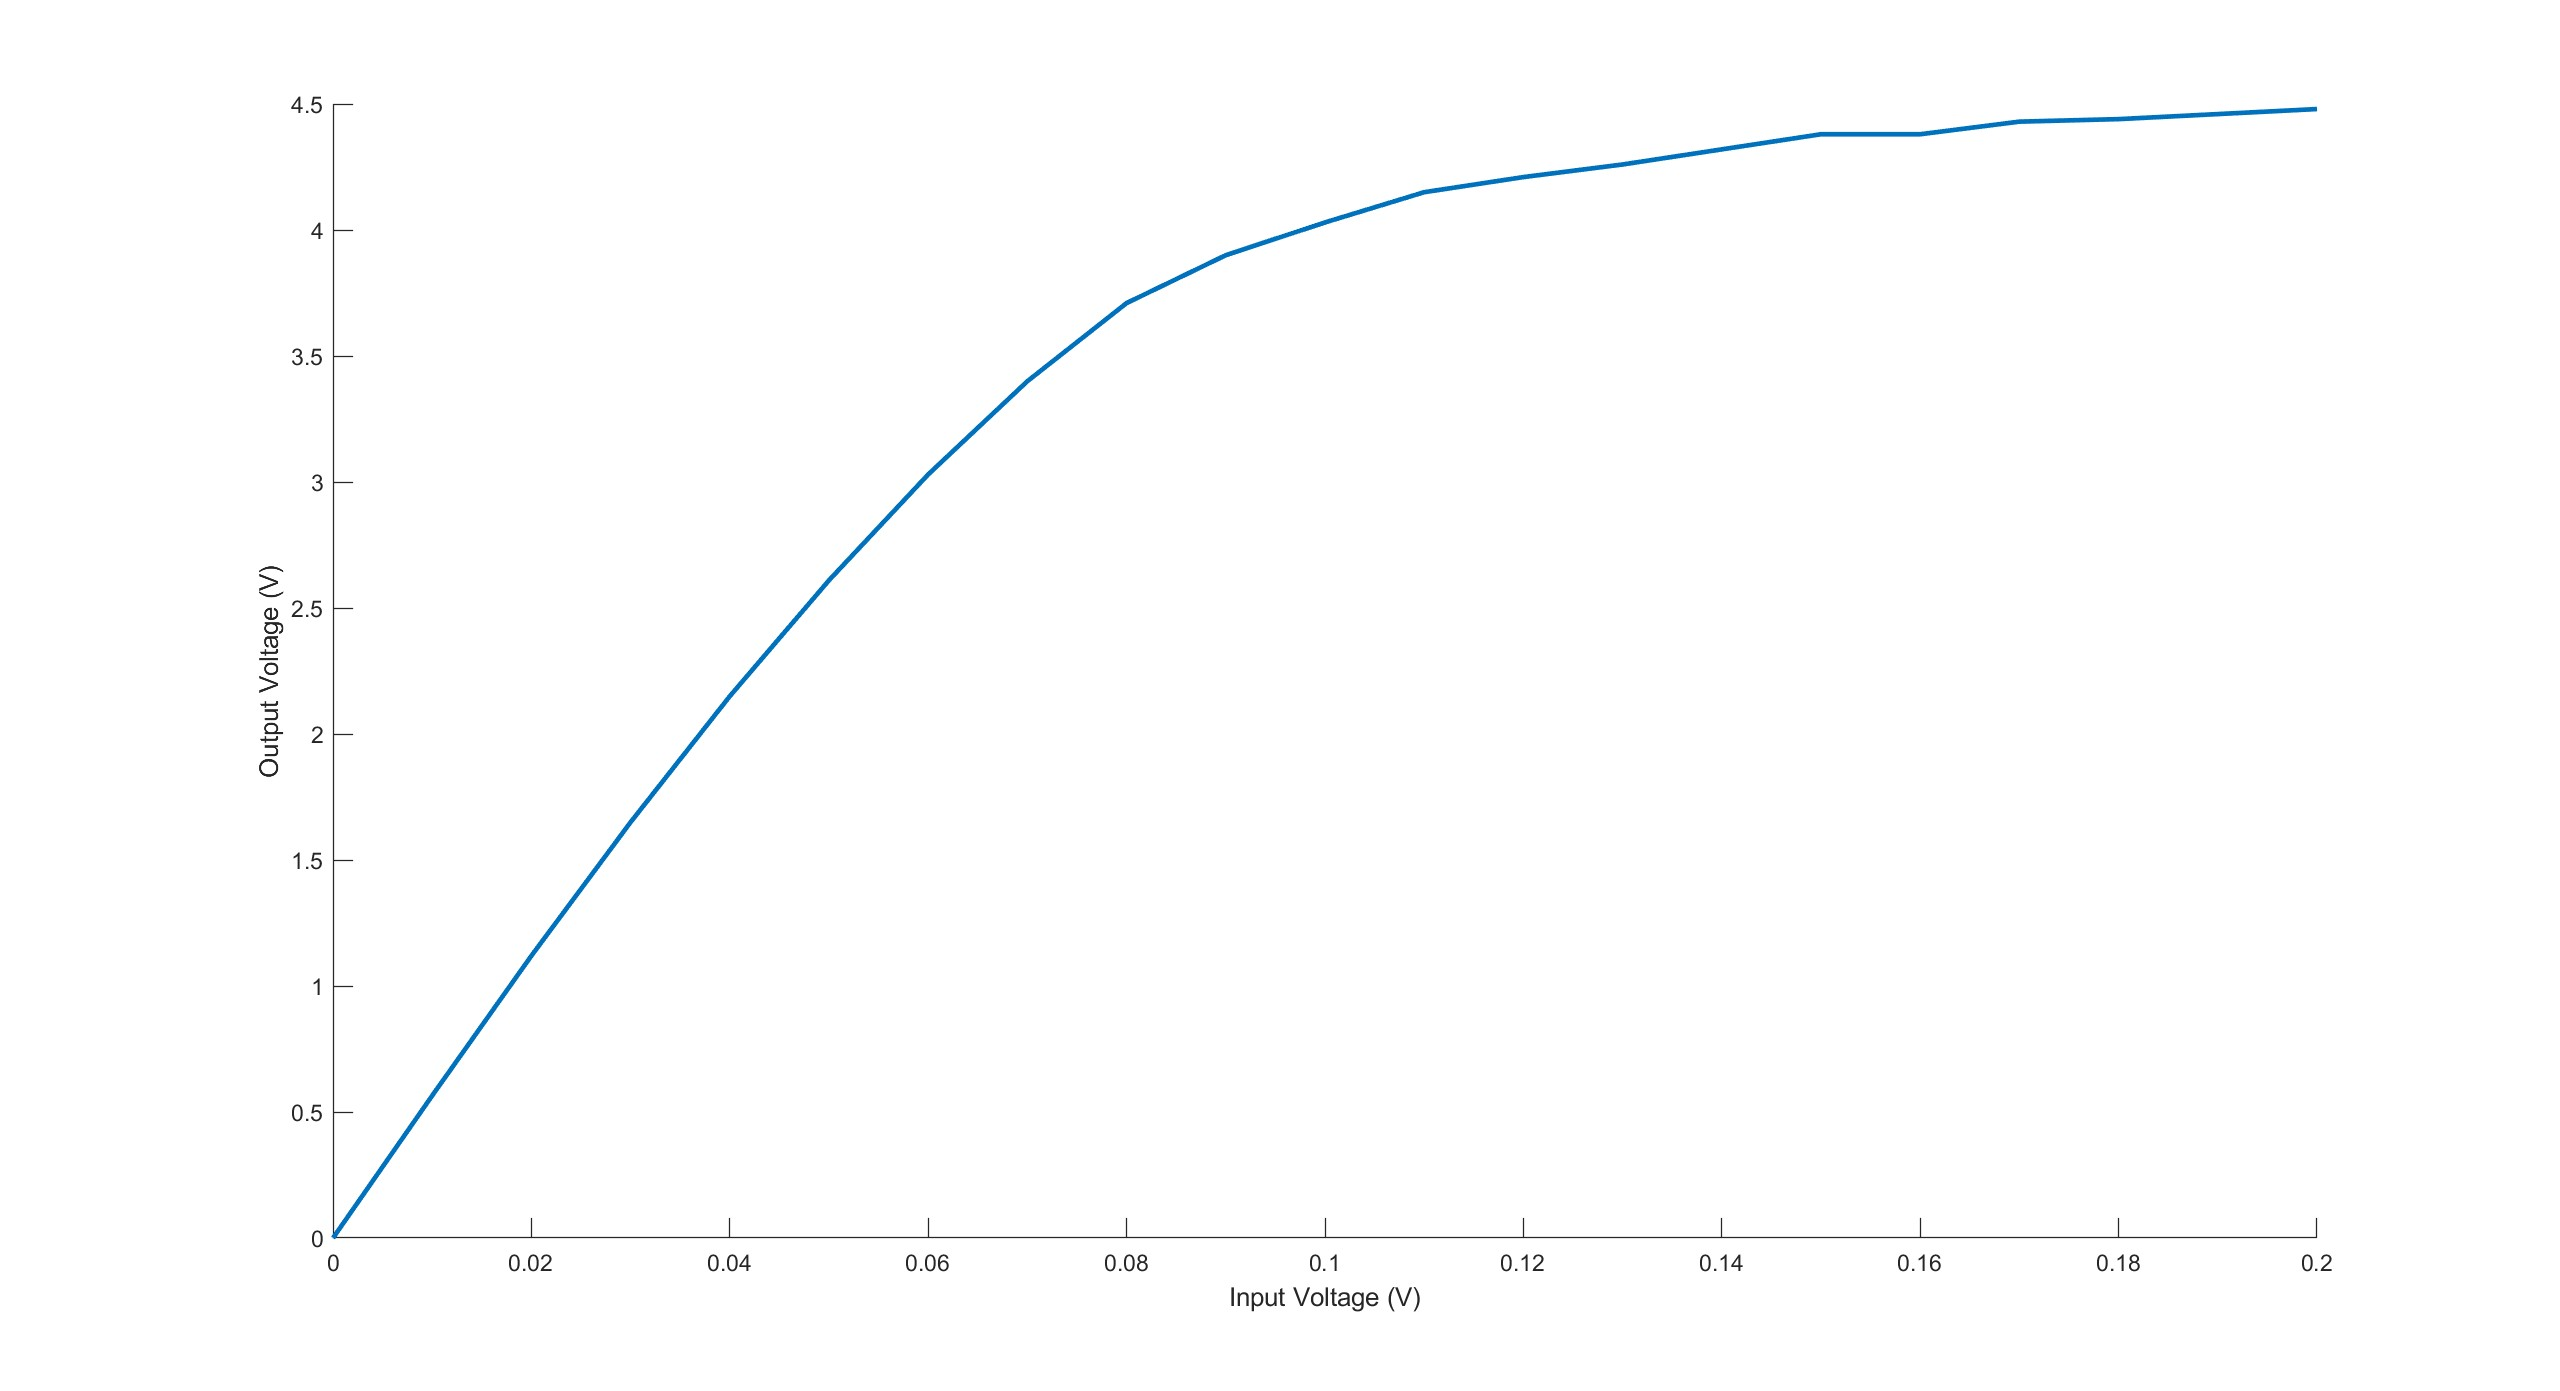
\includegraphics[height=0.31\textwidth]{Images/part_1_voltage_tf.jpg}\\
\caption{Voltage Transfer Curve}
\label{fig:voltagetransfercurve}
\end{figure}
From the voltage transfer curve, we can find the slope of the linear portion, which appears to occur when the input voltage is between 0-0.05V. We find that the slope is \boxed{\frac{2.5}{0.05} = 50\frac{V}{V}}, which matches our design specification of $|A_V| = 50\frac{V}{V}$.

\subsection{Part 1 D}

To measure our input and output impedance, we set our input amplitude to 0.01V, and measure the currents and voltage at both the input and output of our amplifier. We will be shorting the $50\Omega$ source impedance to measure the currents and voltages. For the output we will be shorting the load and measuring the current, and opening the connection to the load to measure the voltage. From there we calculate the input and output impedance from our measured values. 
\begin{center}
$R_{out} = \frac{V_{out}}{I_{out}} = \frac{600mV}{250\mu A}$ = \boxed{2.4k\Omega}, $R_{in} = \frac{V_{in}}{I_{in}} =\frac{7.07mV}{1.4\mu A}$ = \boxed{5050\Omega} 
\end{center}

We can conclude that our output and input impedance matches our design specification, as the specification is $R_{out} = R_C$ and $R_{in} = 5k\Omega$


%----------------------------Part 2-------------------------------

\section{Part 2 - Cascaded Amplifiers}

\begin{figure}[h!]
\centering
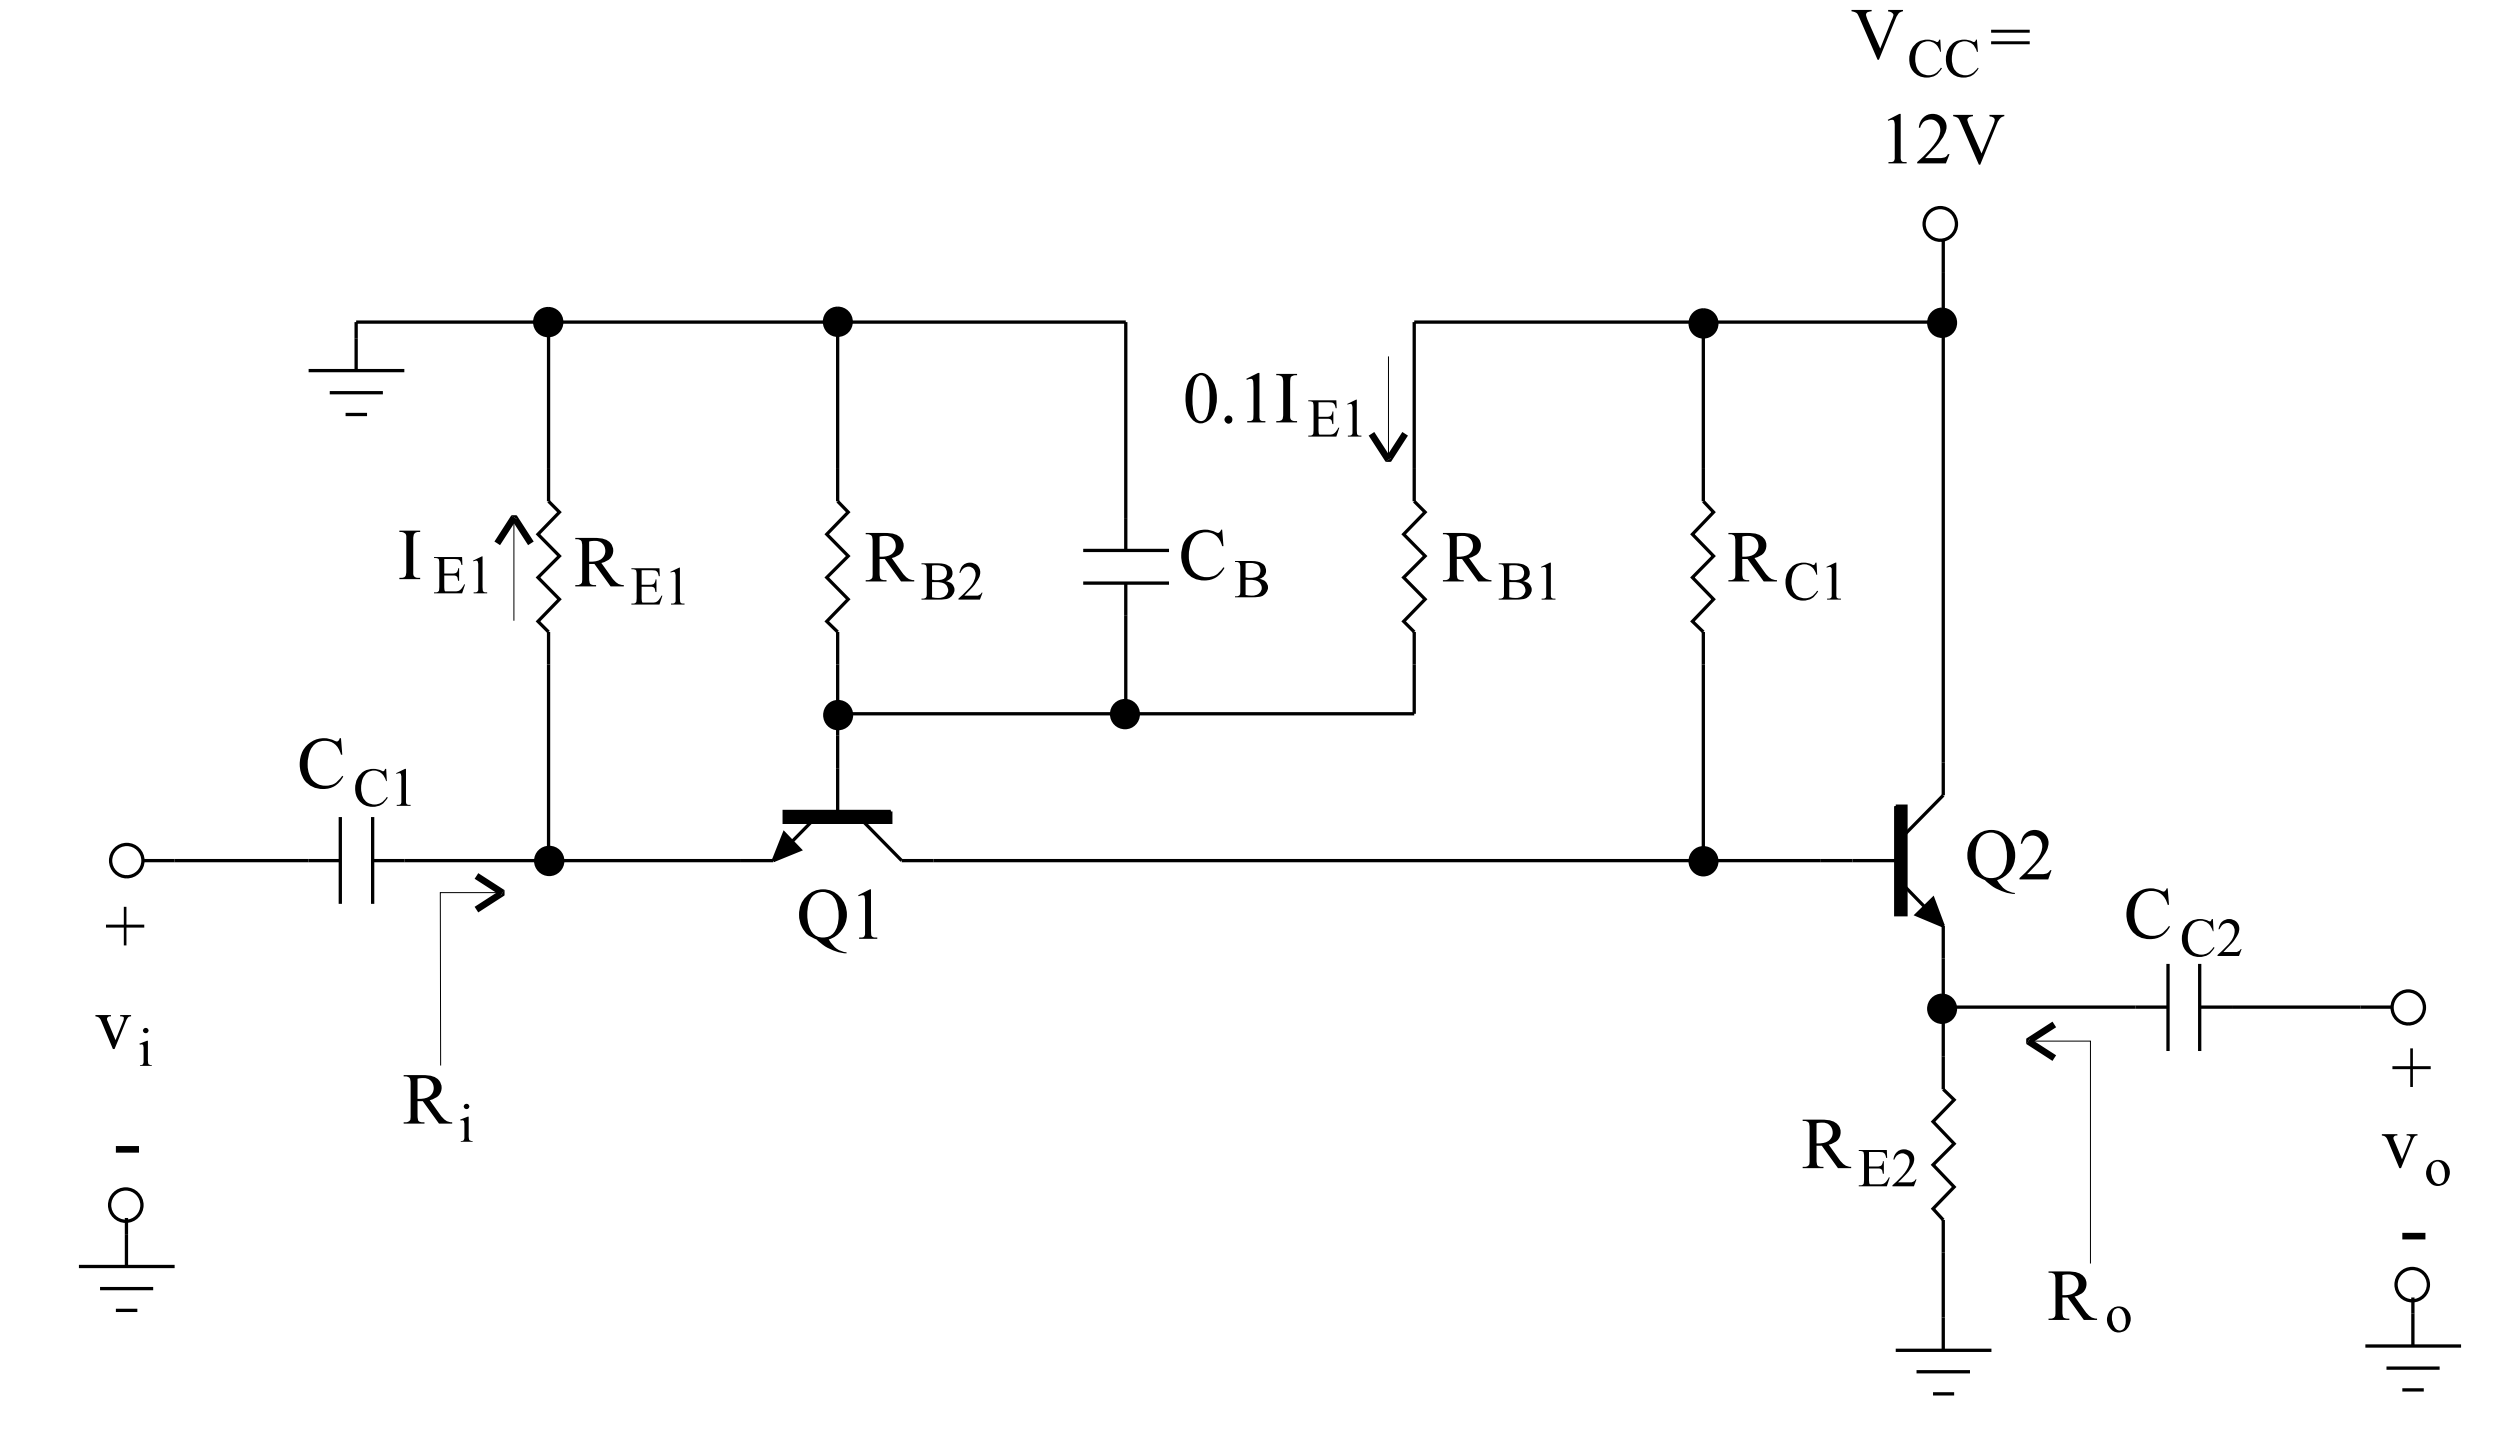
\includegraphics[height=0.25\textwidth]{Images/part_2_circuit.png}\\
\caption{Cascaded Common Base/Common Collector Amplifier}
\label{fig:cascadedamplifier}
\end{figure}




For our cascaded amplifier circuit, we will be taking $\beta =300$ as used previously. We will be designing our circuit so that the input and output impedance is 50±5$\Omega$. We will still be using 2N3904 transistors for our circuit. 

\subsection{Part 2 A}
To design our circuit, we will be using $V_{CC}$=12V and the 1/3 rule; where $V_{E1} = \frac{V_{CC}}{3}$
and $I_1=0.1I_{E1}$. We will also be setting $w_{L3dB} = 1000*2\pi$ rad/s.

Here is the circuit we will be using to bias our transistors:

\begin{figure}[h!]
\centering
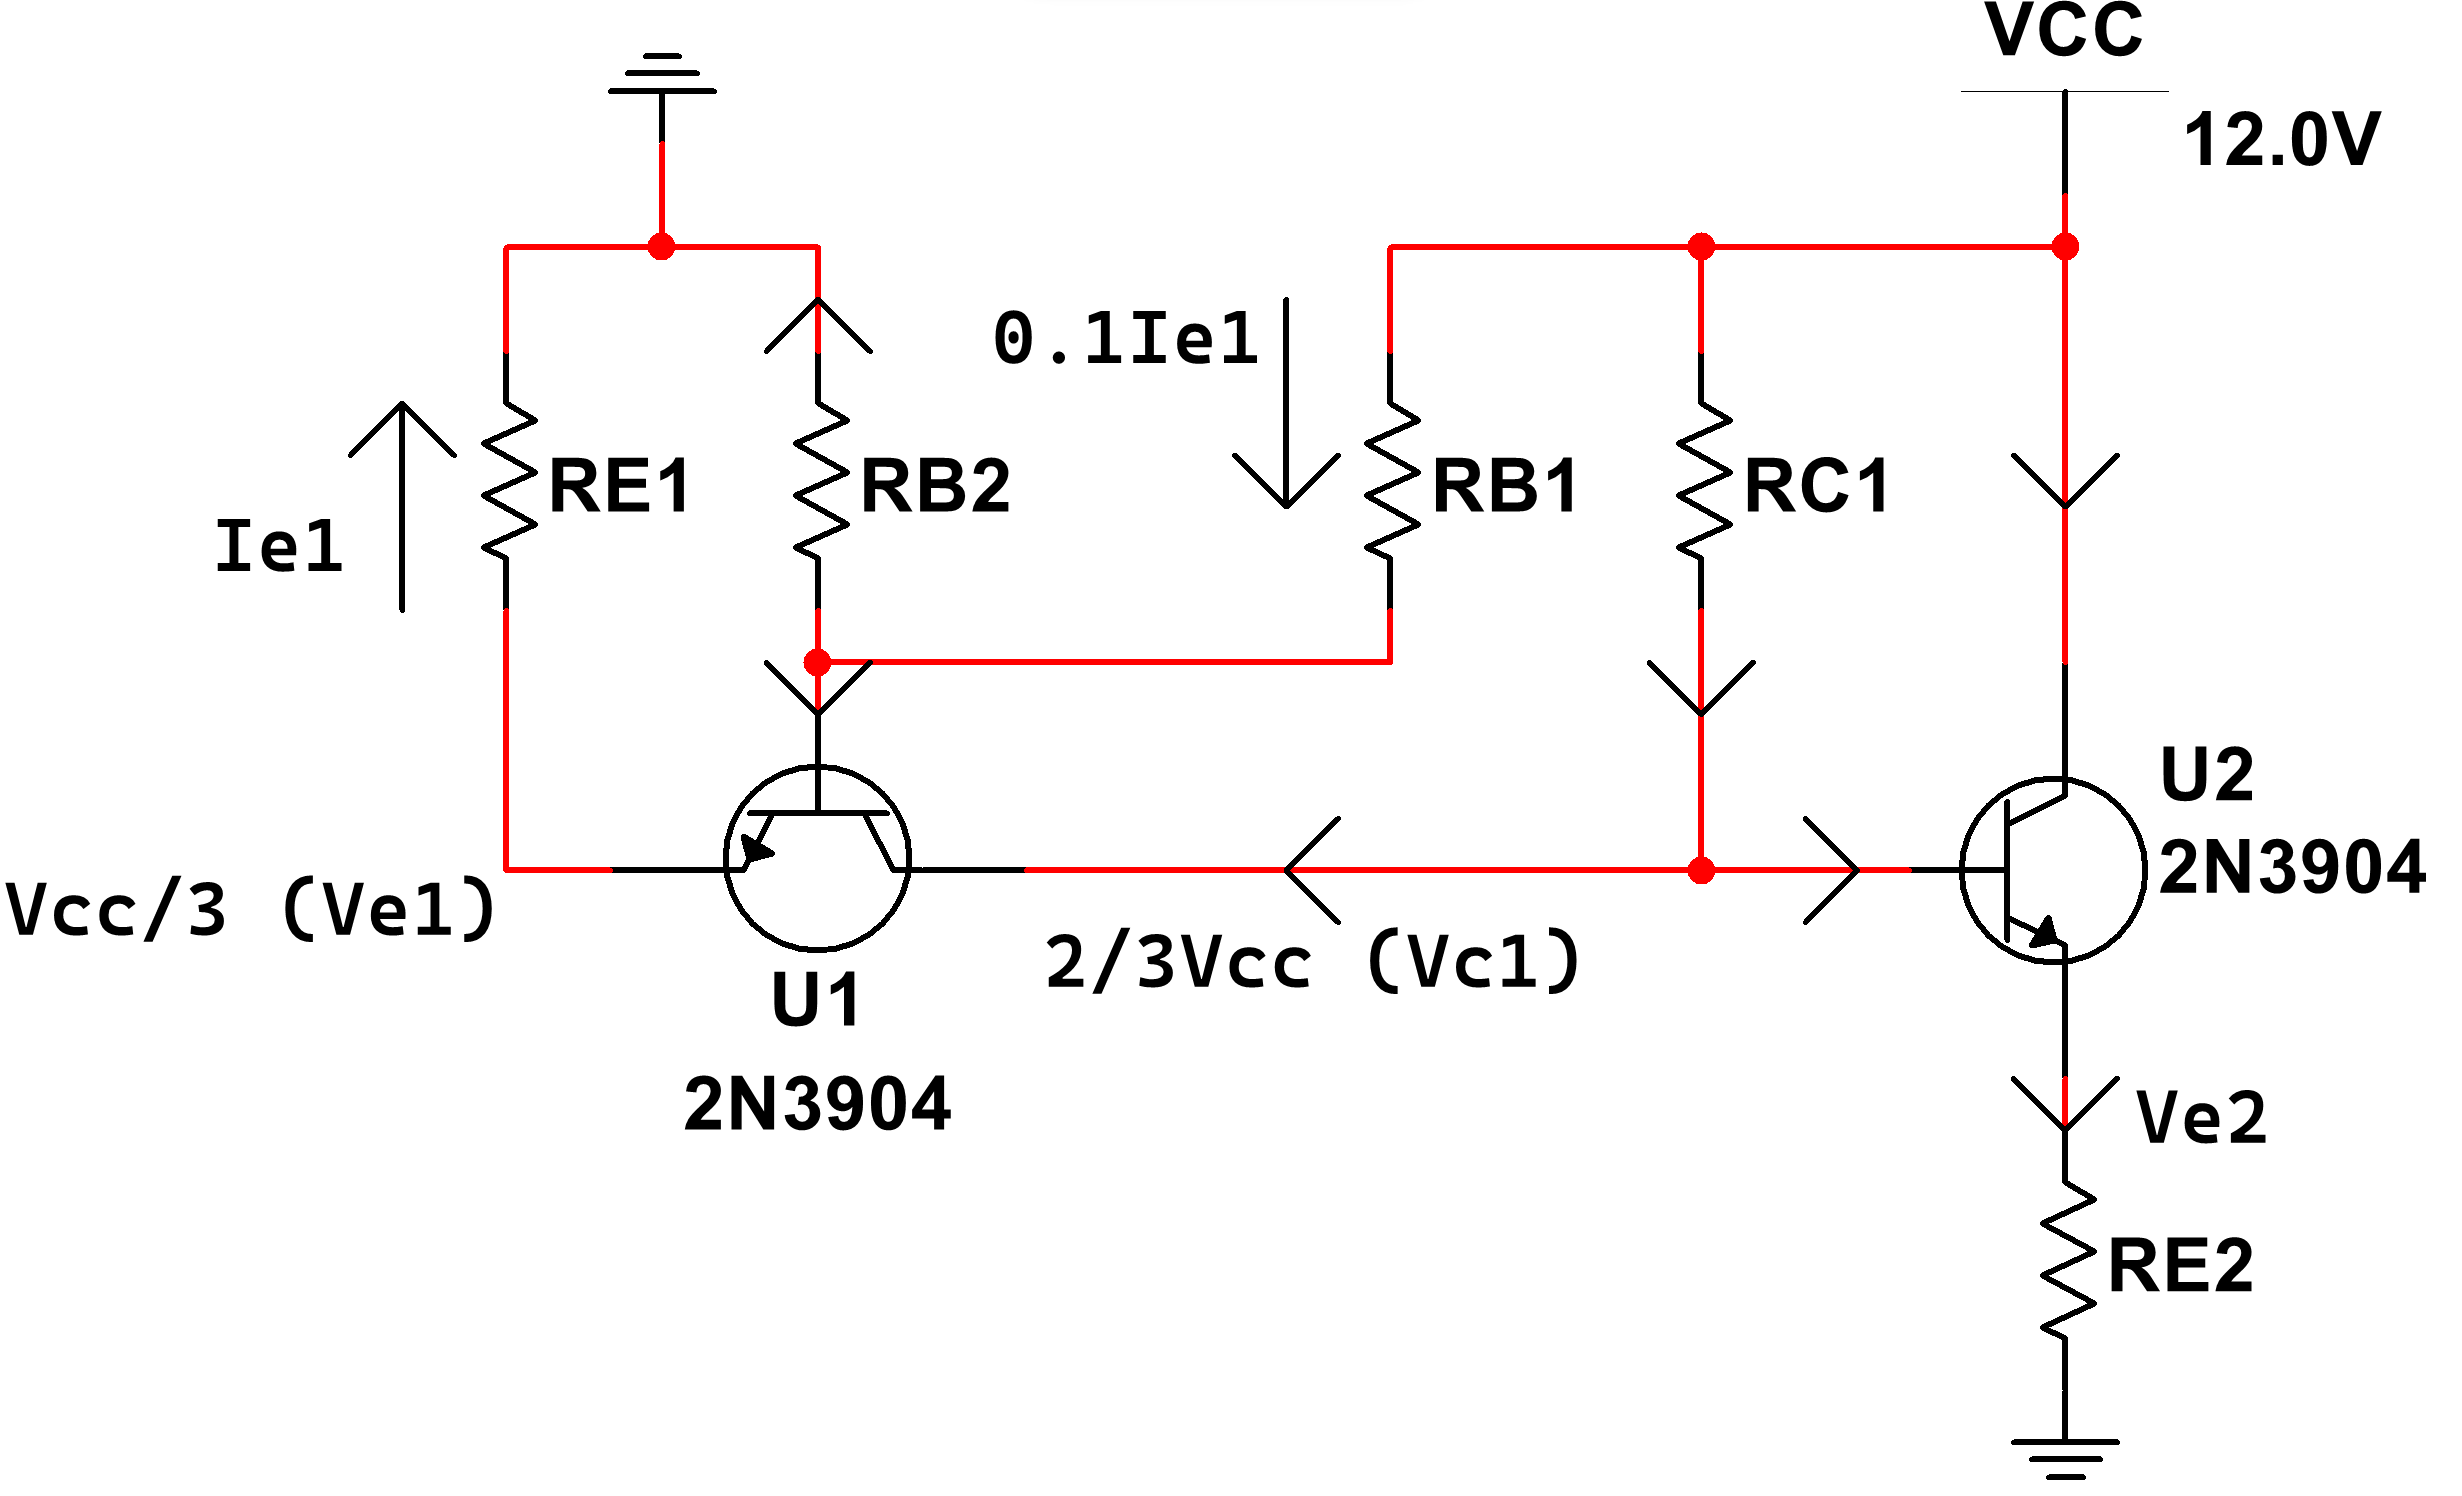
\includegraphics[height=0.25\textwidth]{Images/part_2_bias.png}\\
\caption{DC Cascaded Circuit}
\label{fig:1/4rulecircuit}
\end{figure}
\FloatBarrier

From the mid-band model shown below, we can derive formula for input and output resistance:
\begin{figure}[h!]
\centering
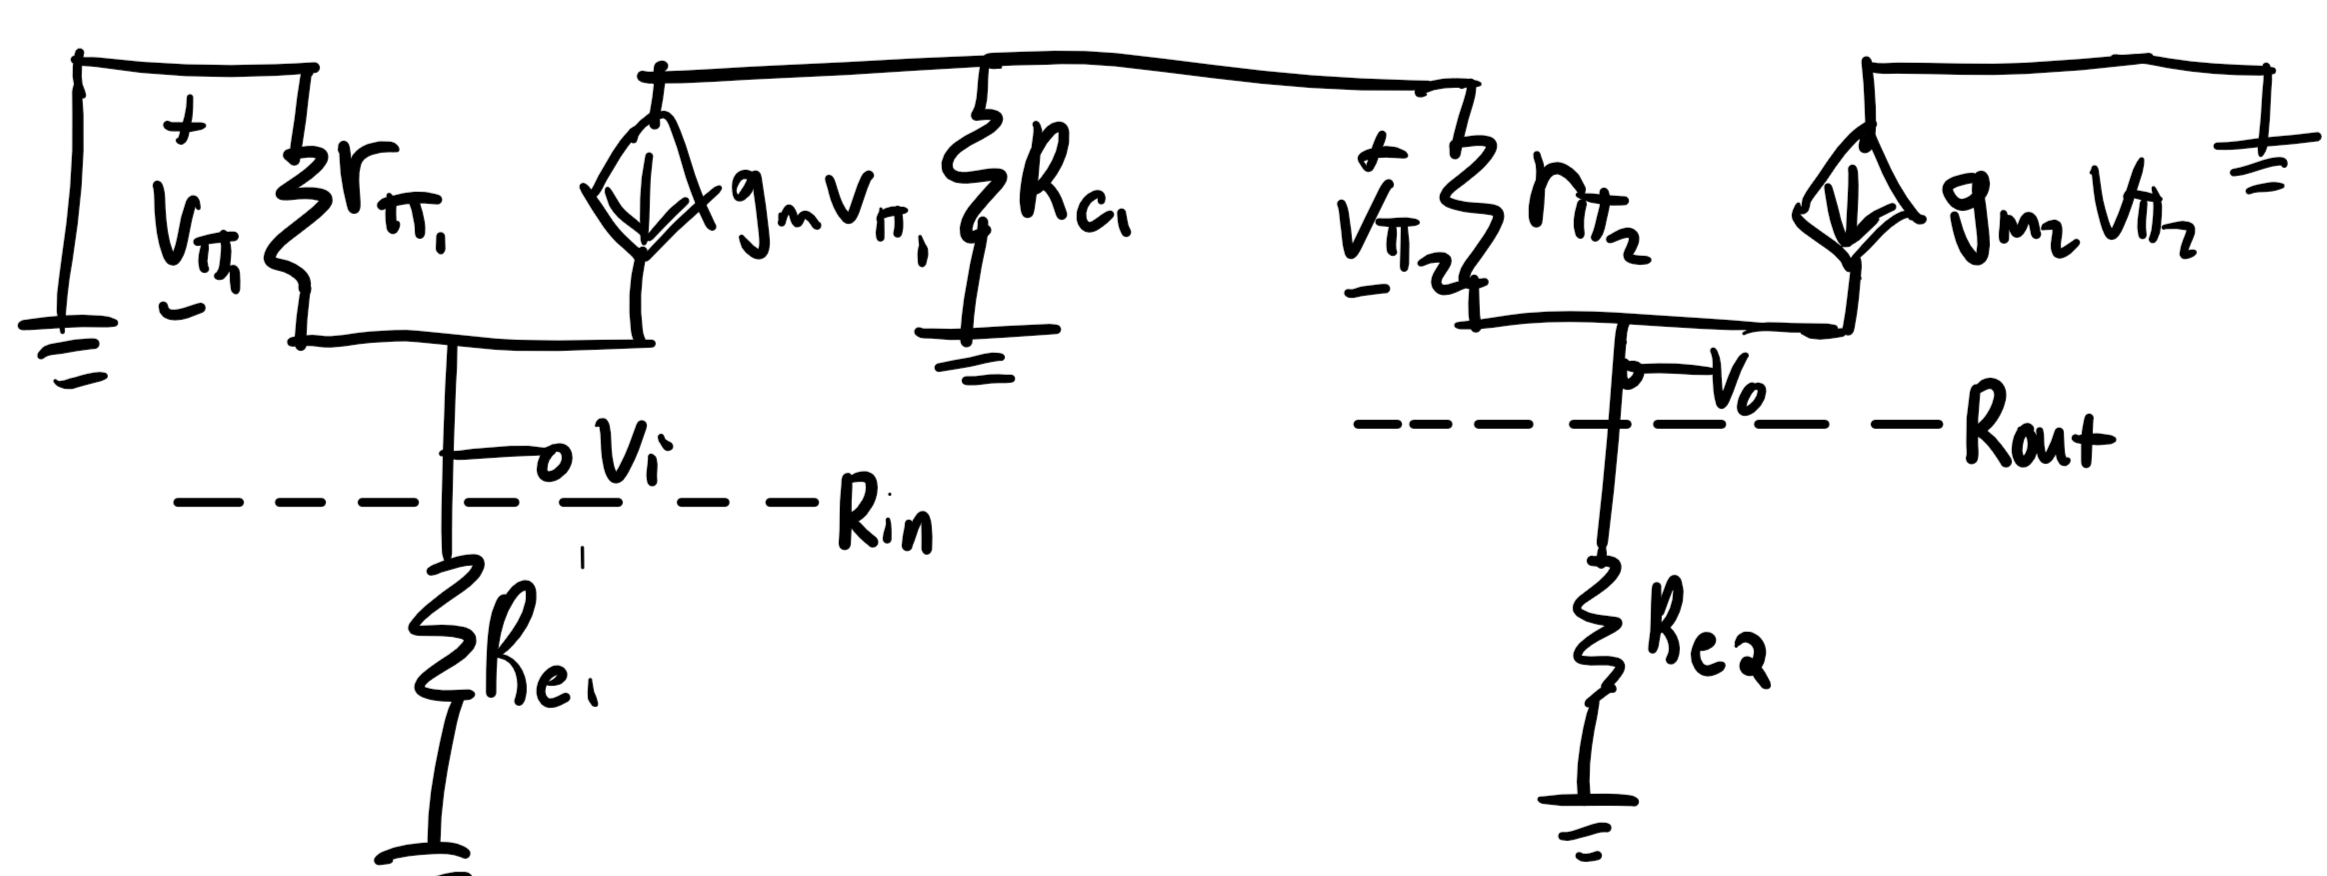
\includegraphics[height=0.15\textwidth]{Images/part_2_midband.png}\\
\caption{Mid-band Small Signal Model}
\label{fig:1/4rulecircuit}
\end{figure}

We can observe that $R_{in}=\frac{r_\pi}{1+\beta}||R_{e1}$ and $R_{out} = \frac{R_{C1}+r_\pi}{1+\beta}||R_{E2}$.


Since we want to set $R_{in}=50=\frac{r_\pi}{1+\beta}$, we can derive a formula for $I_{E1}$. Shown as: 
\begin{center}
$R_{in}=50=\frac{r_\pi}{1+\beta}||R_{E1}$
\end{center}
If we substitute $r_\pi = \beta \frac{V_t}{I_{C1}}$ and $I_{C1} = \frac{I_{E1}}{1+\frac{1}{\beta}}$, we can make an equation to solve for $I_{E1}$:
\begin{center}
$50\Omega = \frac{(\frac{r\pi}{1+\beta})R_{E1}}{\frac{r\pi}{1+\beta}+R_{E1}} =  \frac{(\frac{\frac{\beta}{I_{C1}}V_t}{1+\beta})\frac{V_{E1}}{I_{E1}}}{\frac{\frac{\beta}{I_{C1}}V_t}{1+\beta}+\frac{V_{E1}}{I_{E1}}}$ 

\end{center}
 We can solve that $I_{E1}$ is about \boxed{0.5mA}.
\newline
Here are the equations that we will be using to find the currents:
\begin{center}
$I_{B1} = \frac{I_{E1}}{1+\beta}, 
I_{E2} = \frac{V_{E2}}{R_{E2}},    
I_{B2} = \frac{\frac{V_{E2}}{R_{E2}}}{\beta +1}$
\end{center}


To find $R_{E2}$, we use the output resistance:
\newline
\begin{center}
$R_{out} = \frac{R_{C1}+r_{\pi2}}{1+\beta}||R_{E2} = 50\Omega$
\end{center}

Knowing that $R_{C1} = \frac{V_{CC}-V_{B2}}{I_{C1}+I_{B2}}$, and $r_{\pi2} = \frac{\beta V_t}{I_{C2}}$ we can substitute in our equations as shown, and use $R_{C1}$ written in terms of $R_{E2}$. Therefore we can find that  $R_{E2} = 6.9732k\Omega$. We can substitute that value in to then solve for the other impedance:
\begin{flalign}
&R_{B1}=\frac{V_{CC}-V_{B1}}{0.1I_{E1}} = \boxed{146k\Omega} \nonumber\\
&R_{B2}=\frac{V_{B1}}{0.1I_{E1}-I_{B1}} = \boxed{97.230k\Omega} \nonumber\\
&R_{E1}=\frac{V_{E1}}{I_{E1}} = \boxed{8k\Omega} \nonumber
\end{flalign}

From here we can use the low frequency circuit to find the dominant poles, and then the capacitance of the capacitors.


\begin{figure}[h!]
\centering
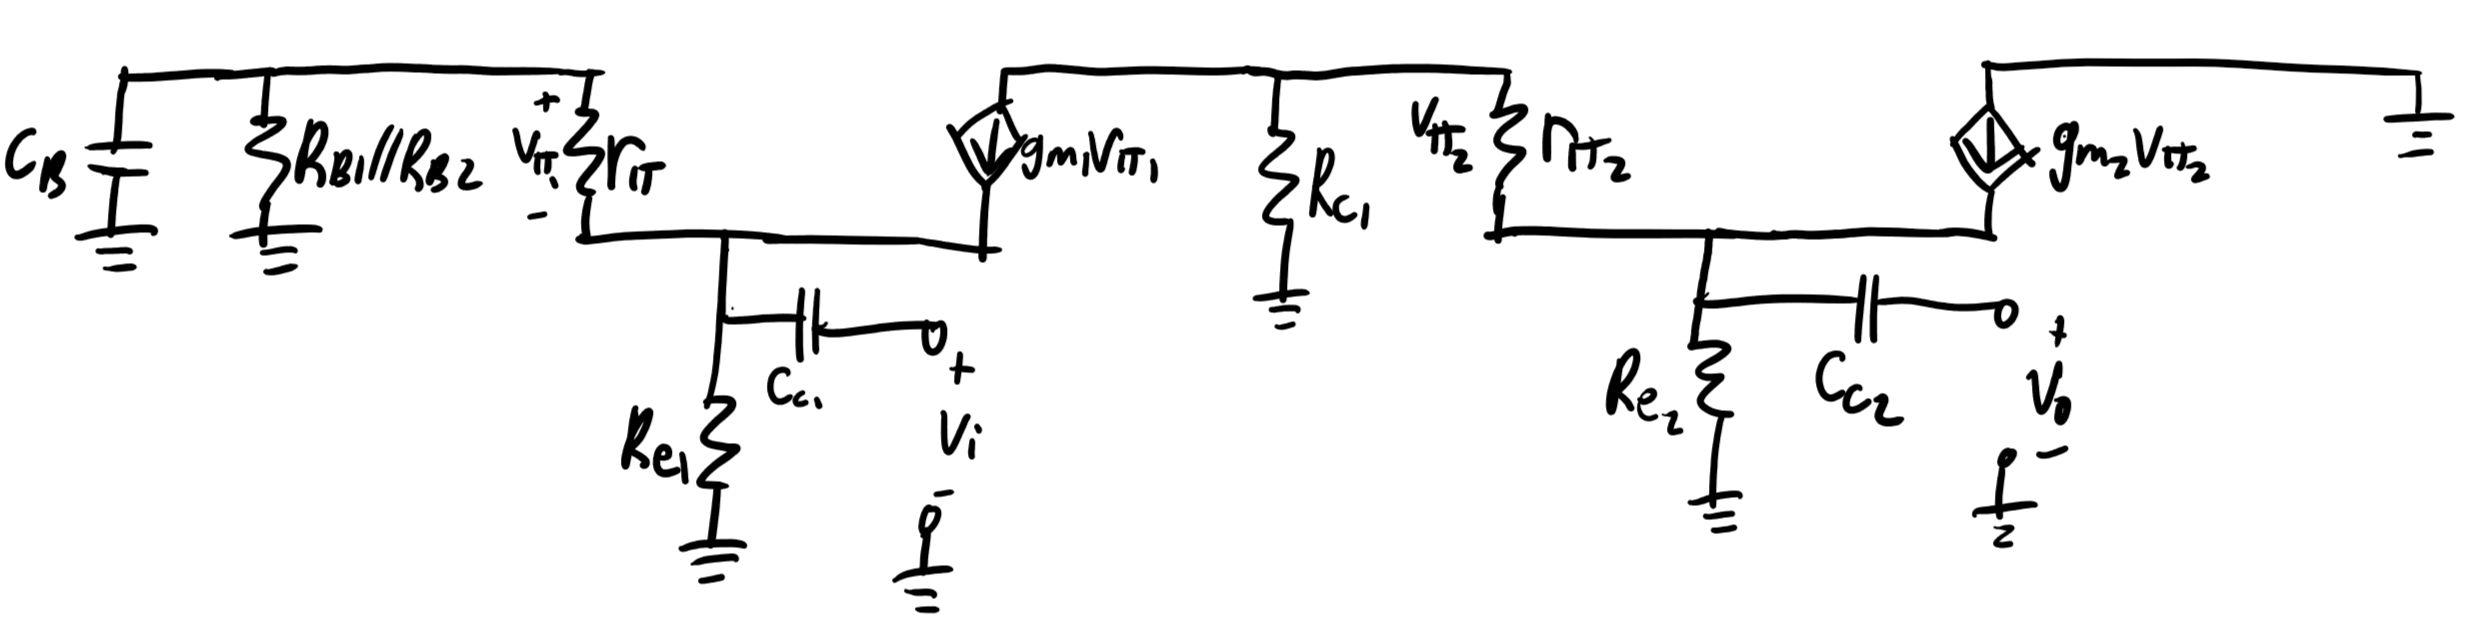
\includegraphics[height=0.15\textwidth]{Images/part_2_lowf.png}\\
\caption{Low Frequency Small Signal Model}
\label{fig:lowfcircuit}
\end{figure}

Here we will be finding the resistance seen by the capacitors using the open circuit the short circuit tests. Because of the locations of the $c_{C1}$ and $C_{C2}$ capacitors, we find that the calculations for the resistance seen by the capacitors are identical to the calculation used to find the input and output impedance. Because the specification requires that the input and output impedance be $50\Omega$ we can assume that the resistance seen by $C_{C1}$ and $C_{C2}$ are also $50\Omega$. Because of that, we can determine that the capacitance of $C_{C1}$ and $C_{C2}$ are identical as well. Since the values seen by the capacitors are also relatively low, we can also assume that they are the dominant poles in this amplifier. Therefore we can use the following calculation to find the values of the capacitors:
\begin{flalign}
&1000*2\pi=\sqrt{(\frac{1}{50*C_{C1}})^2+(\frac{1}{50*C_{C2}})^2}\nonumber \\
&C_{C1}=C_{C2} = \boxed{4.502\mu F} \nonumber
\end{flalign}

To find $C_B$ with the lowest possible capacitance, we set the pole location 1 decade below the dominant pole, so that it does not contribute. So if $w_{LP2} = \frac{1}{C_{C1}(50)} = 4.444k rad/s$, we will set $w_{LP1} = 444 rad/s$. When $C_B$ is active, the other low frequency capacitors will act as open circuits. The calculation is shown below:
\begin{center}
$\tau_{C_B} = C_B(R_{B2}||R_{B1}||r_{\pi1}+(1+\beta)R_{E1}))$
\newline
$444=\frac{1}{\tau_{C_B}}$
\end{center}
Solving the above equation for $C_B$, we find that it is about \boxed{39.48nF}.

\subsection{Part 2 B}
Now that we have all of our values, we can now convert everything to standard values and create our circuit.



\begin{table}[h!]
\centering
\begin{tabular}{l|l|l|l|l|l|l|l}

           & $R_{B1}$     & $R_{B2}$        & $R_{E1}$     & $R_{E2}$       & $R_{C1}$       & $C_{C1/C2}$ & $C_B$       \\ \cline{2-8}
Calculated & 146k$\Omega$ & 97.230k$\Omega$ & 8k$\Omega$   & 6.972k$\Omega$ & 7.971k$\Omega$ & 4.5$\mu$F   & 40nF        \\
Standard   & 150k$\Omega$ & 100k$\Omega$    & 8.2k$\Omega$ & 6.8k$\Omega$   & 8.2k$\Omega$   & 4.7$\mu$F   & 0.039$\mu$F
\end{tabular}
\caption{Bias Resistor and Capacitor Values}
\label{Bias Resistor and Capacitor Values}
\end{table}
To measure our input and output impedance, we will be measuring with 100kHz at 1mV to measure at mid-band. To measure the input, we will be putting our source at the input, and grounding our output. To measure the output, we will be moving our source to the output, and grounding the input, both times measuring the current and voltage at the input and output.
Here is the circuit we will be using to measure the input and output impedance:
\begin{figure}[h!]
\centering
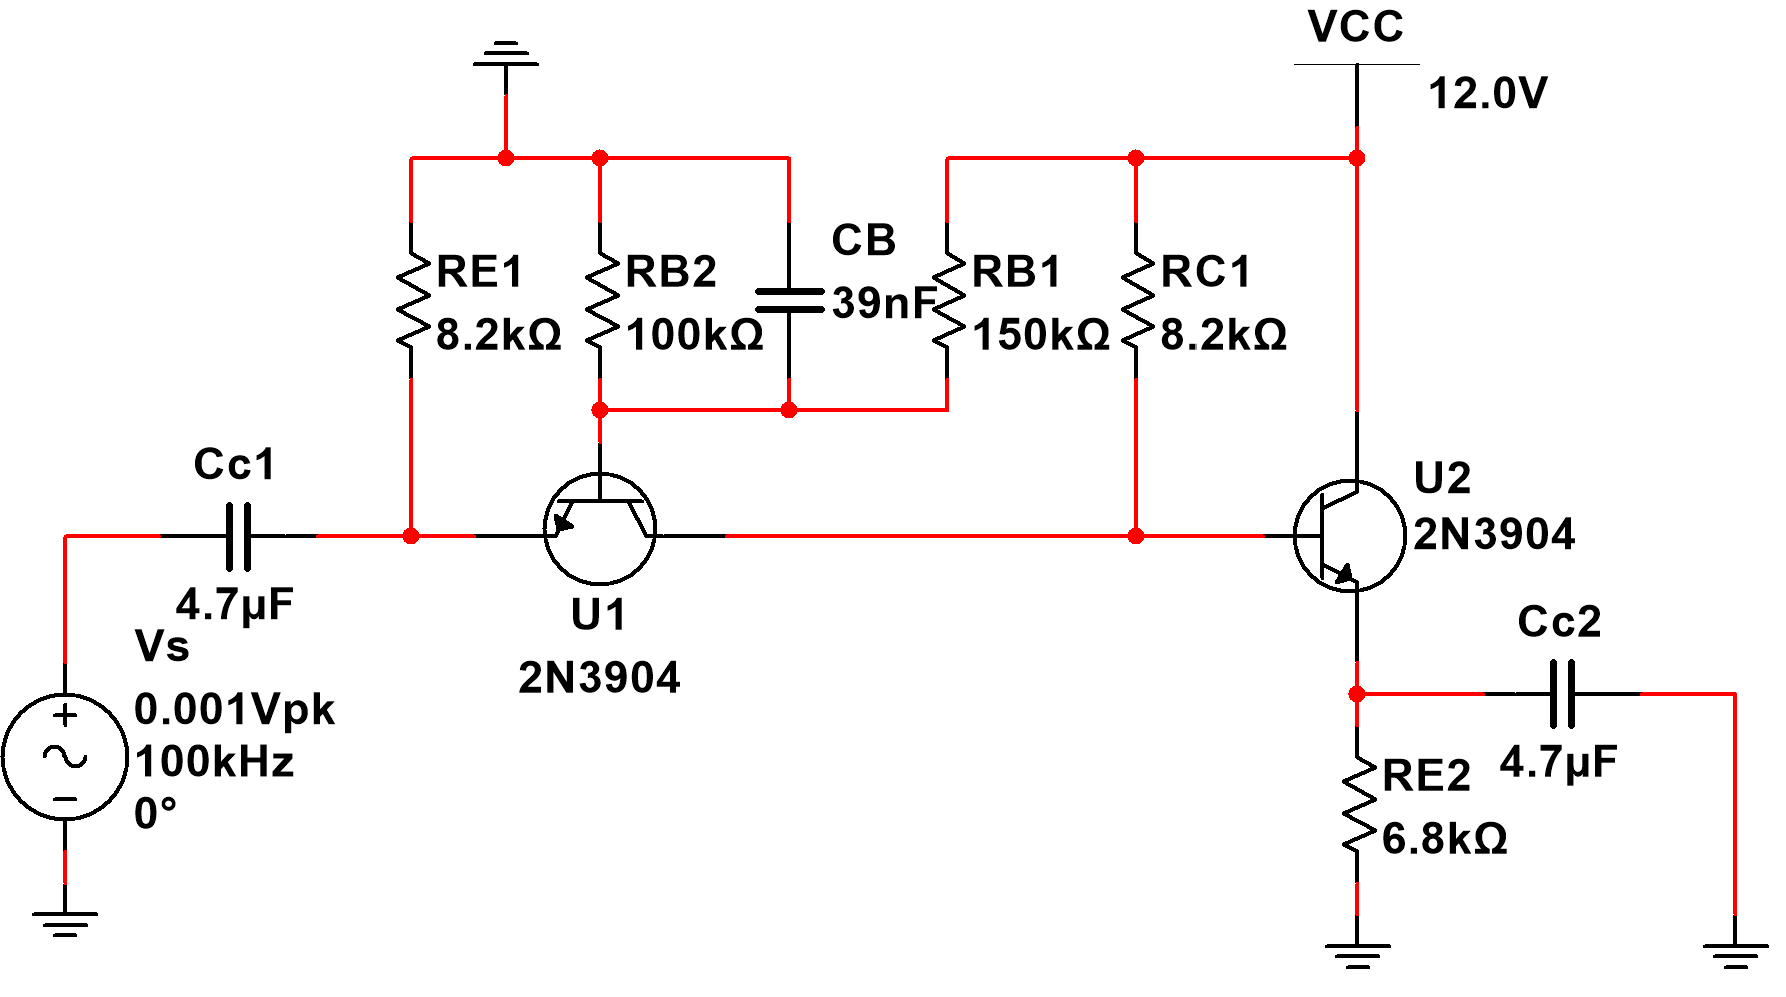
\includegraphics[height=0.25\textwidth]{Images/part_2_sim.png}\\
\caption{Cascade Circuit With Standard Values}
\label{fig:cascadecircuit}
\end{figure}

Here are calculated input and output impedance, using our measured values:
\begin{center}
    $R_{in} = \frac{2mV}{38.9 \mu A}$ = 
    \boxed{51.4 \Omega}       $R_{out} = \frac{2mA}{38.4 \mu A}$ = \boxed{52.1 \Omega}
\end{center}

To measure the mid-band gain, we measure the input voltage and the output voltage, and calculate as shown:

\begin{center}
    $A_v = \frac{176mV}{2mV}$ = \boxed{88 \frac{V}{V}}
\end{center}

For the output impedance, no changes were needed to meet the design specification. However, for the output  $R_{E1} = 7.5k\Omega$ and $R_{C1} = 4.7k\Omega$ was changed so that the impedance matches the input.
From this result, we can determine that the bias calculations were only accurate for the input impedance, but not for the output impedance. This could be due to inaccuracies using the 1/3 rule. We can determine that after modifying our circuit, our input and output impedance meets the specification.
\subsection{Part 2 C}

Here is the circuit that we will be using to make our magnitude and phase bode plots:


\begin{figure}[h!]
\centering
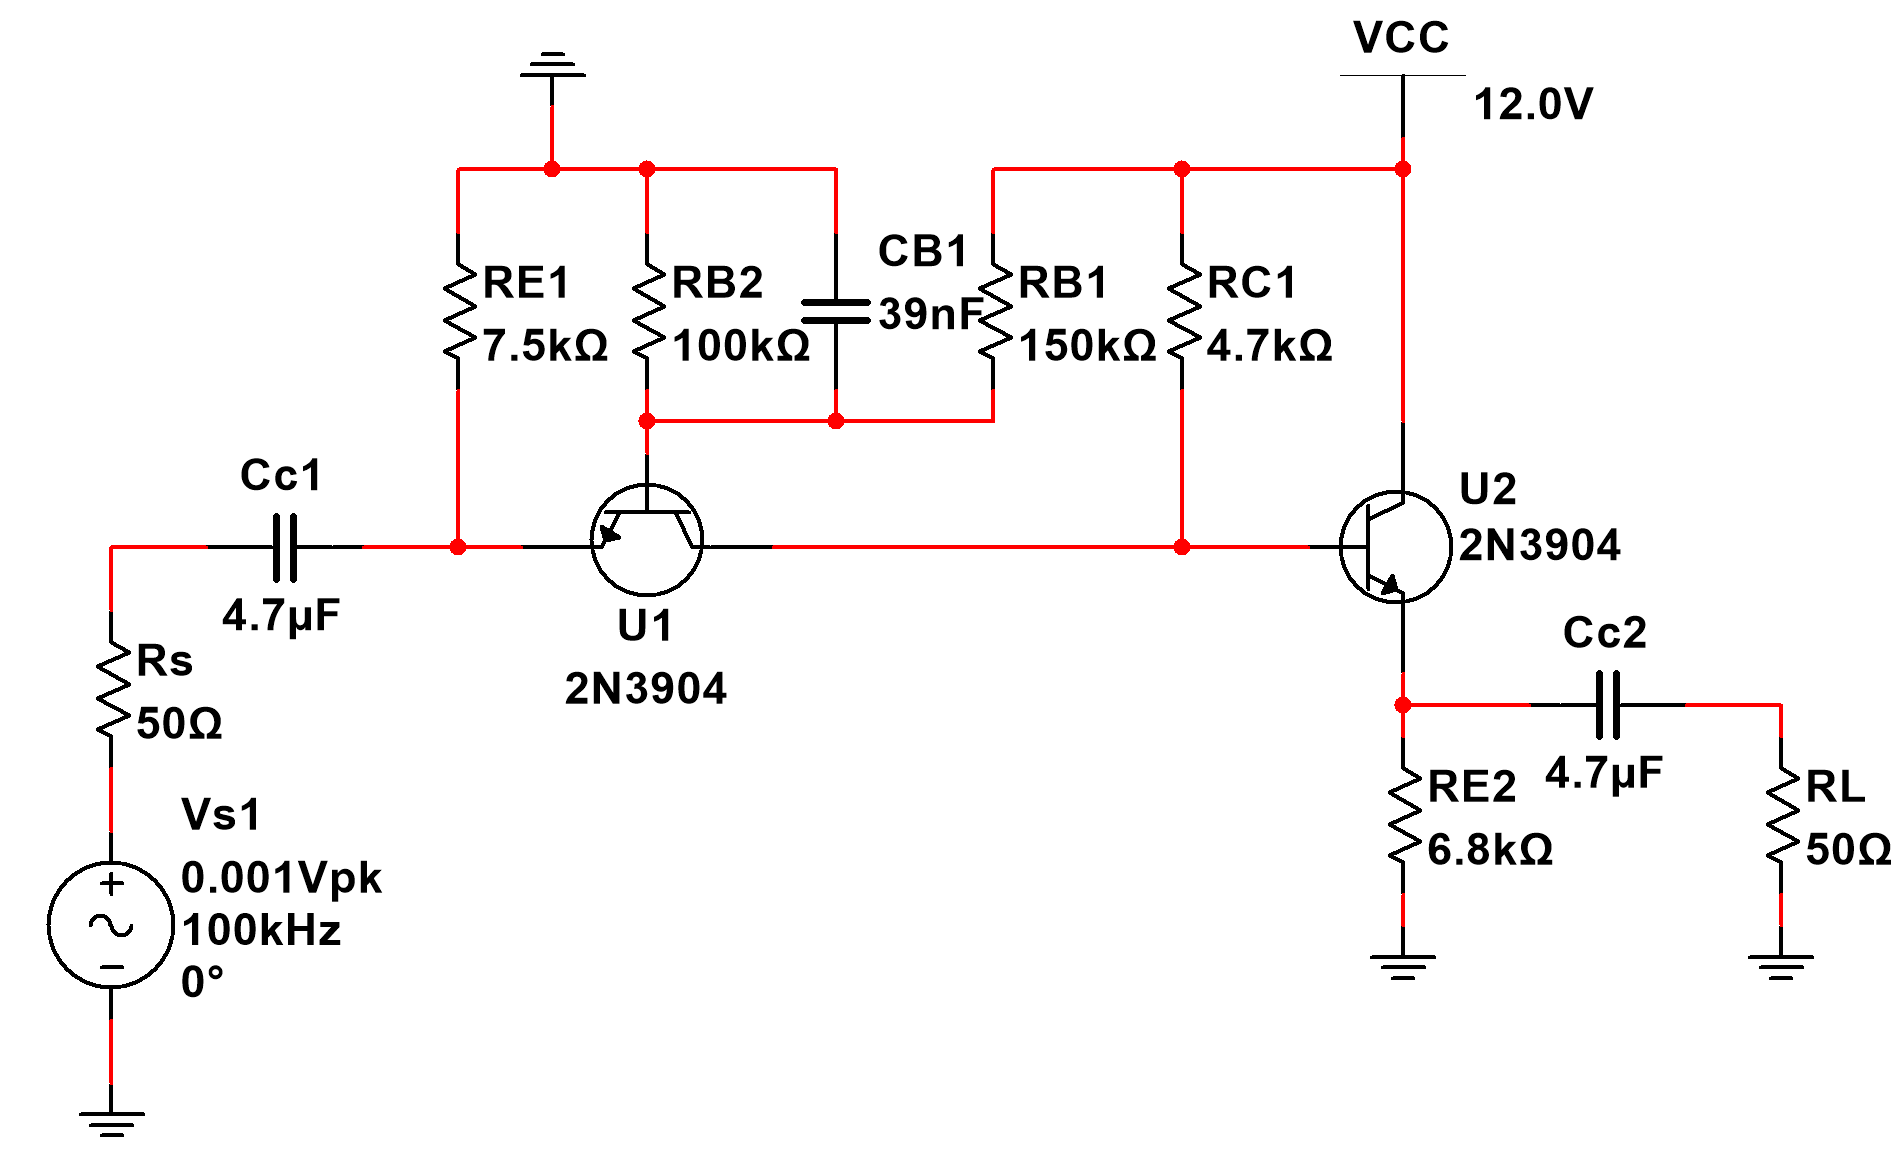
\includegraphics[height=0.25\textwidth]{Images/part_2_bode.png}\\
\caption{Cascade Circuit }
\label{fig:cascadecircuit}
\end{figure}
\FloatBarrier
Here are the magnitude and phase plots:
\begin{figure}[h!]
\centering
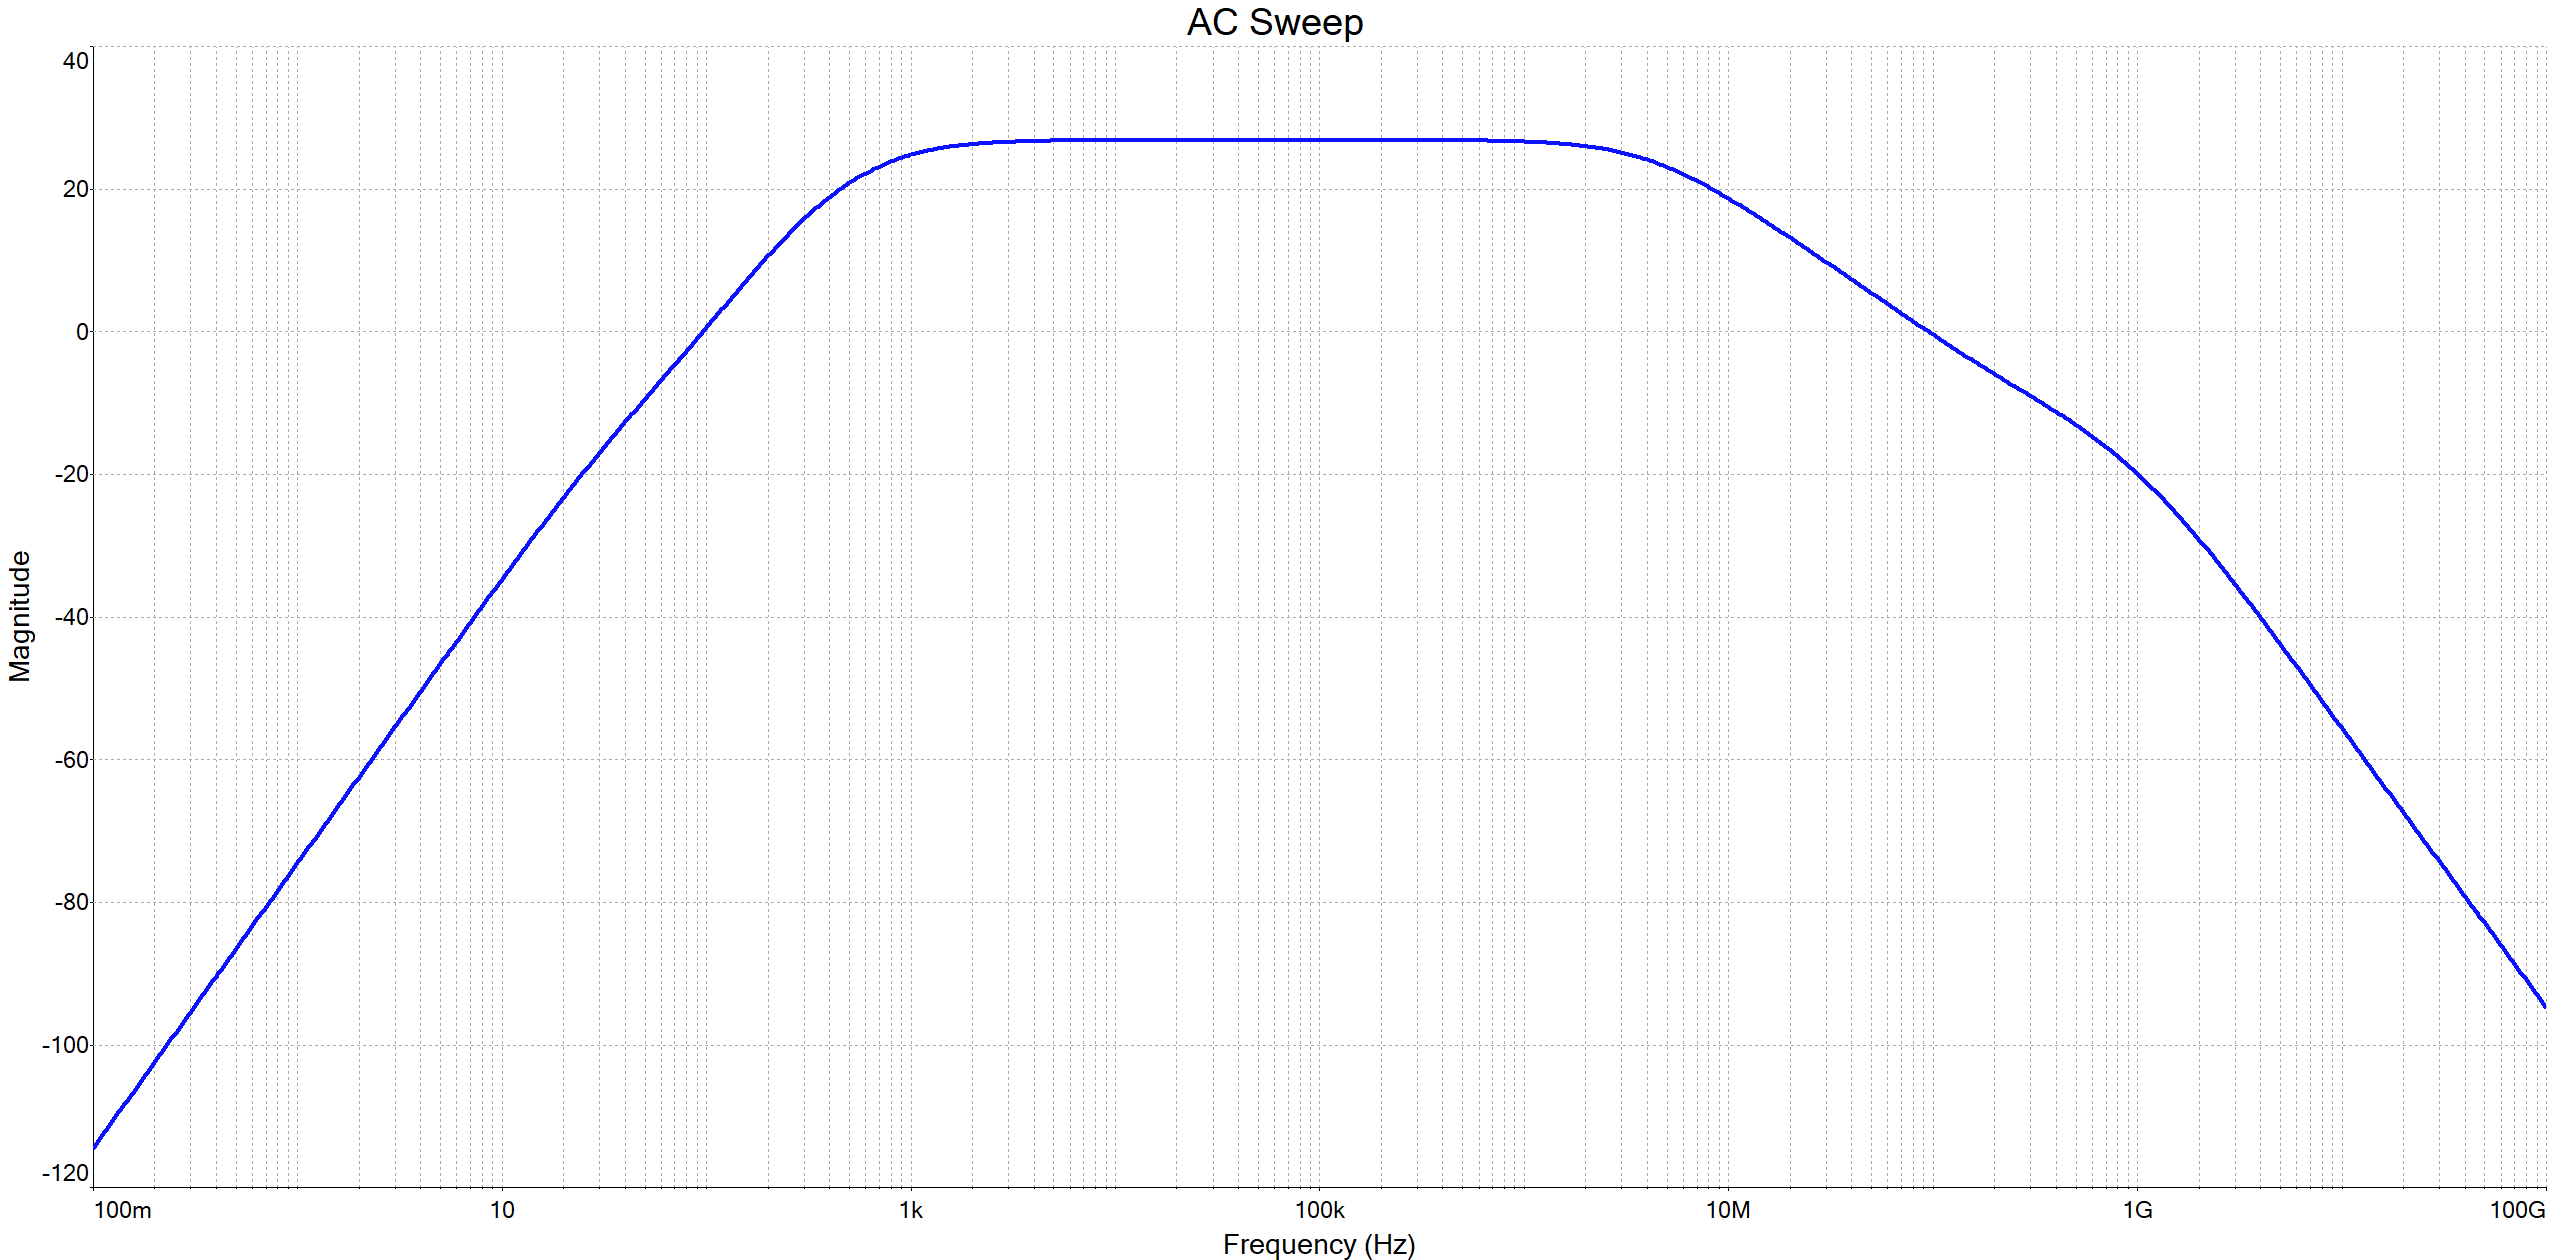
\includegraphics[height=0.4\textwidth]{Images/part_2_bode_plot.png}\\
\caption{Bode Magnitude Plot }
\label{fig:magplot}
\end{figure}
\begin{figure}[h!]
\centering
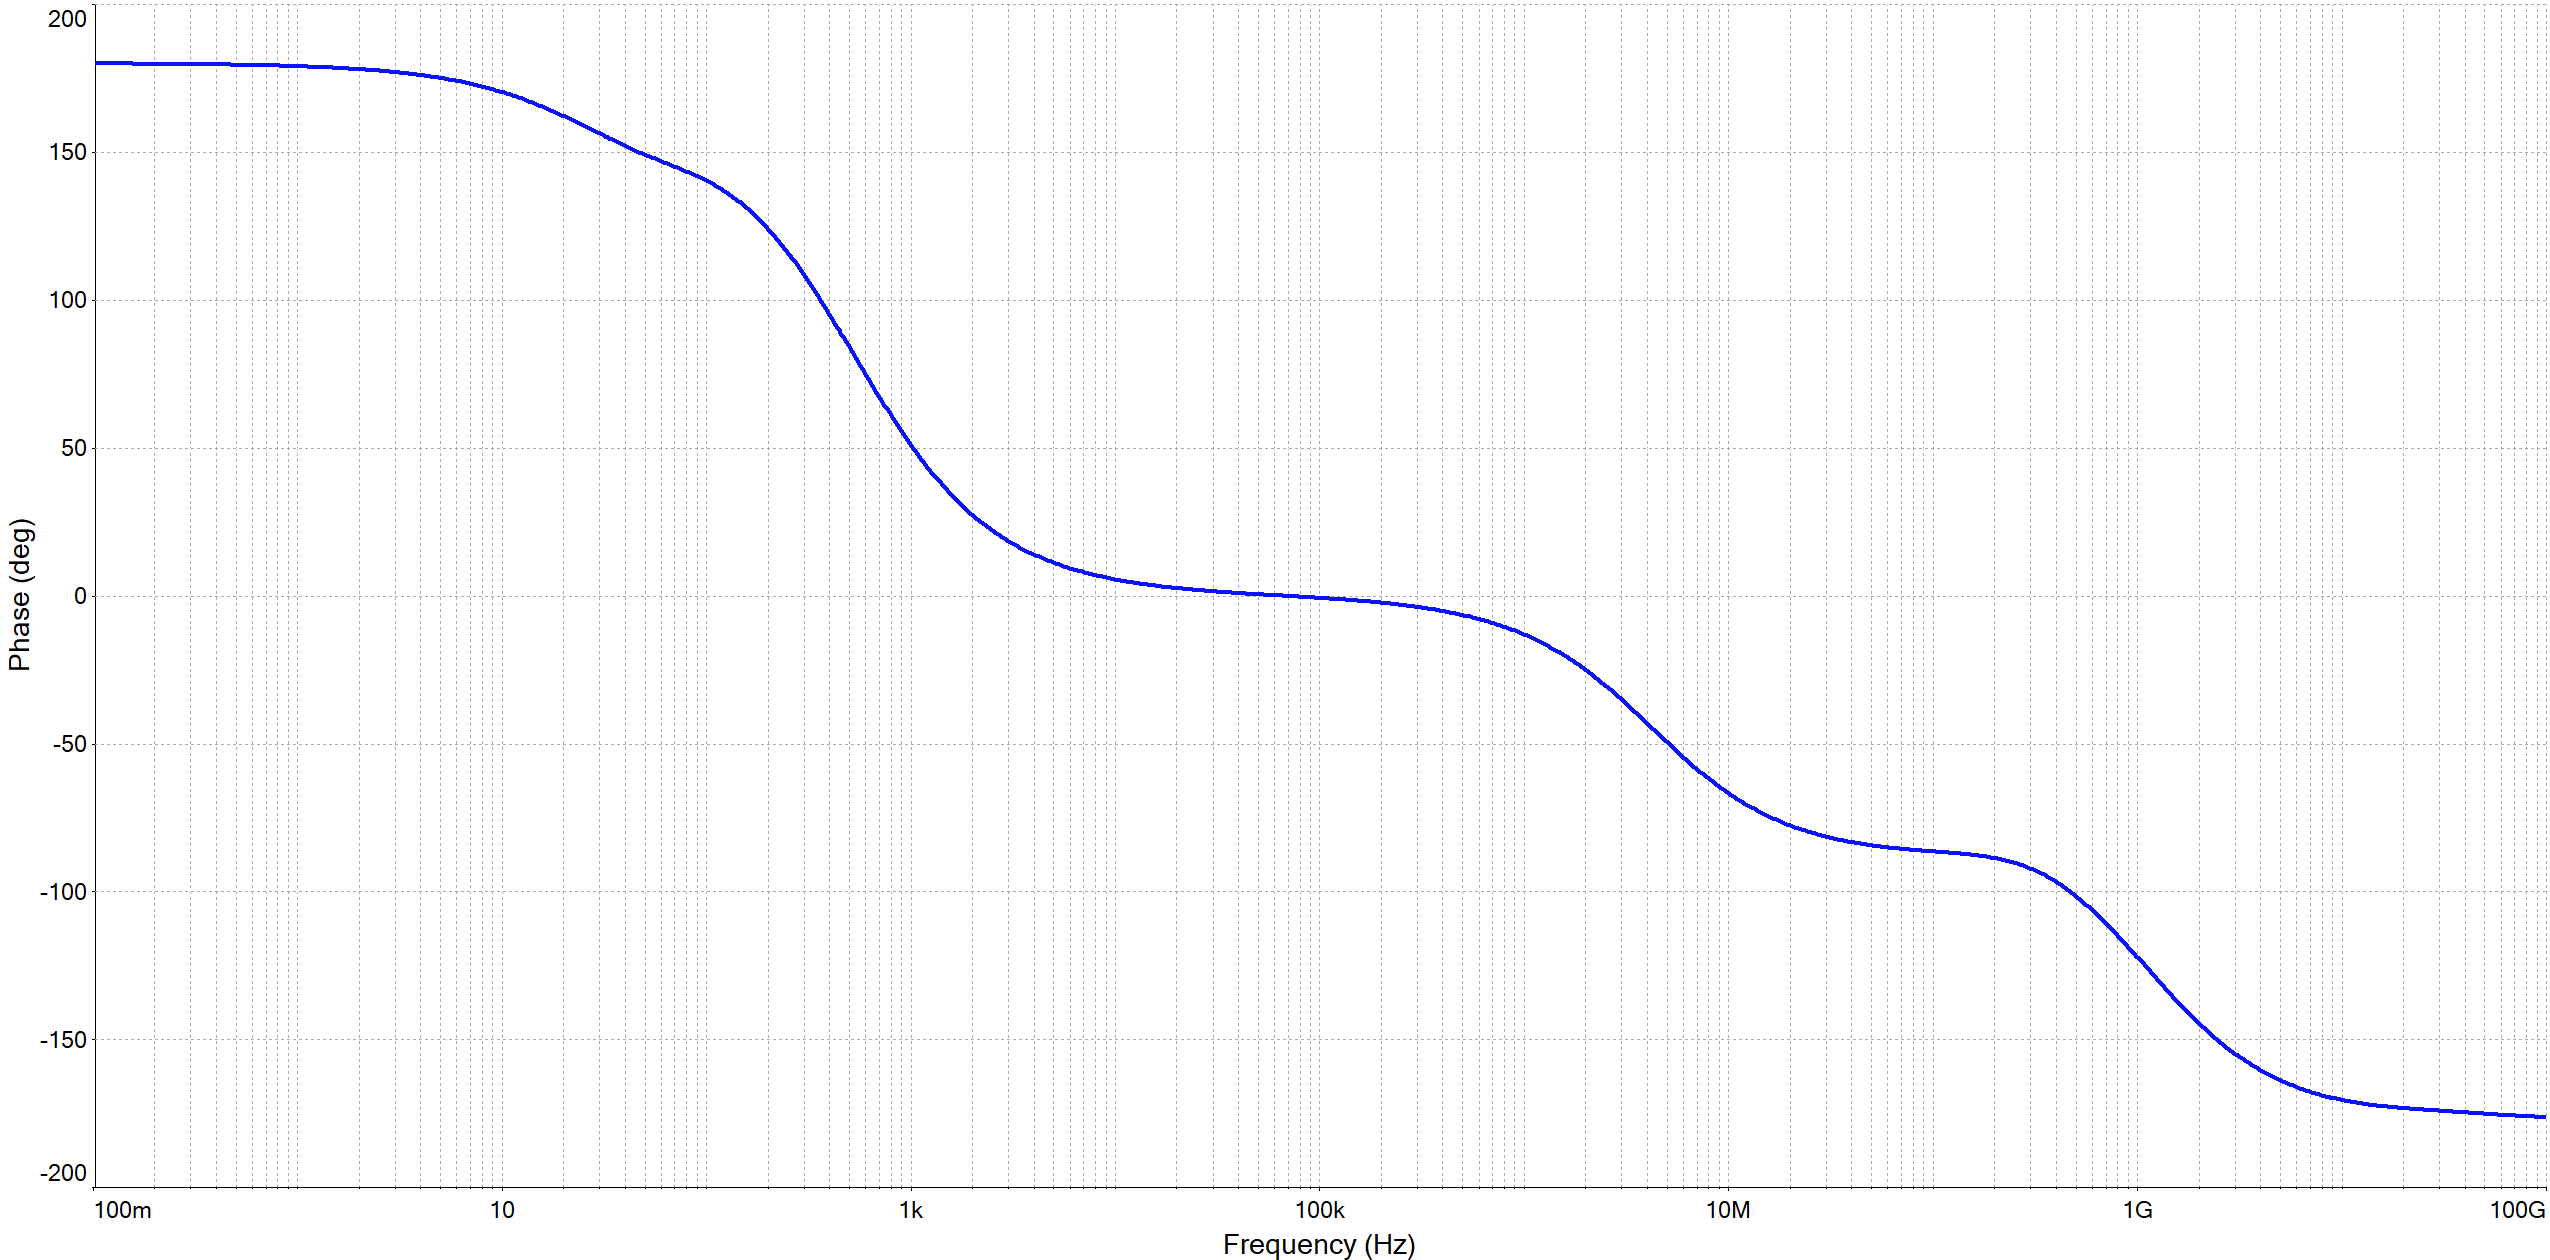
\includegraphics[height=0.35\textwidth]{Images/part_2_phase.png}\\
\caption{Bode Phase Plot}
\label{fig:phaseplot}
\end{figure}
\FloatBarrier
To make the low frequency cut-in match the specification, the low frequency capacitor $C_B$ was changed to 22nF. The high frequency cut-off point was found to be 4.2335*2$\pi$ M rad/s. The measured low frequency cut-off point was found to be 1.03*2$\pi$ k rad/s. We measured our low and high frequency cut-off points using the cursor in Multisim$^{TM}$ and measuring the x-values where the y-value is 3 decibels below the mid-band gain. In conclusion, we can determine that the values of the capacitors with our calculated values are not accurate to the final value used in the actual simulated circuit. However, after modifying our values with respect to our given cut-off frequencies and input and output impedance, our final amplifier design matches the specifications given.
The final circuit used is shown below:

\begin{figure}[h!]
\centering
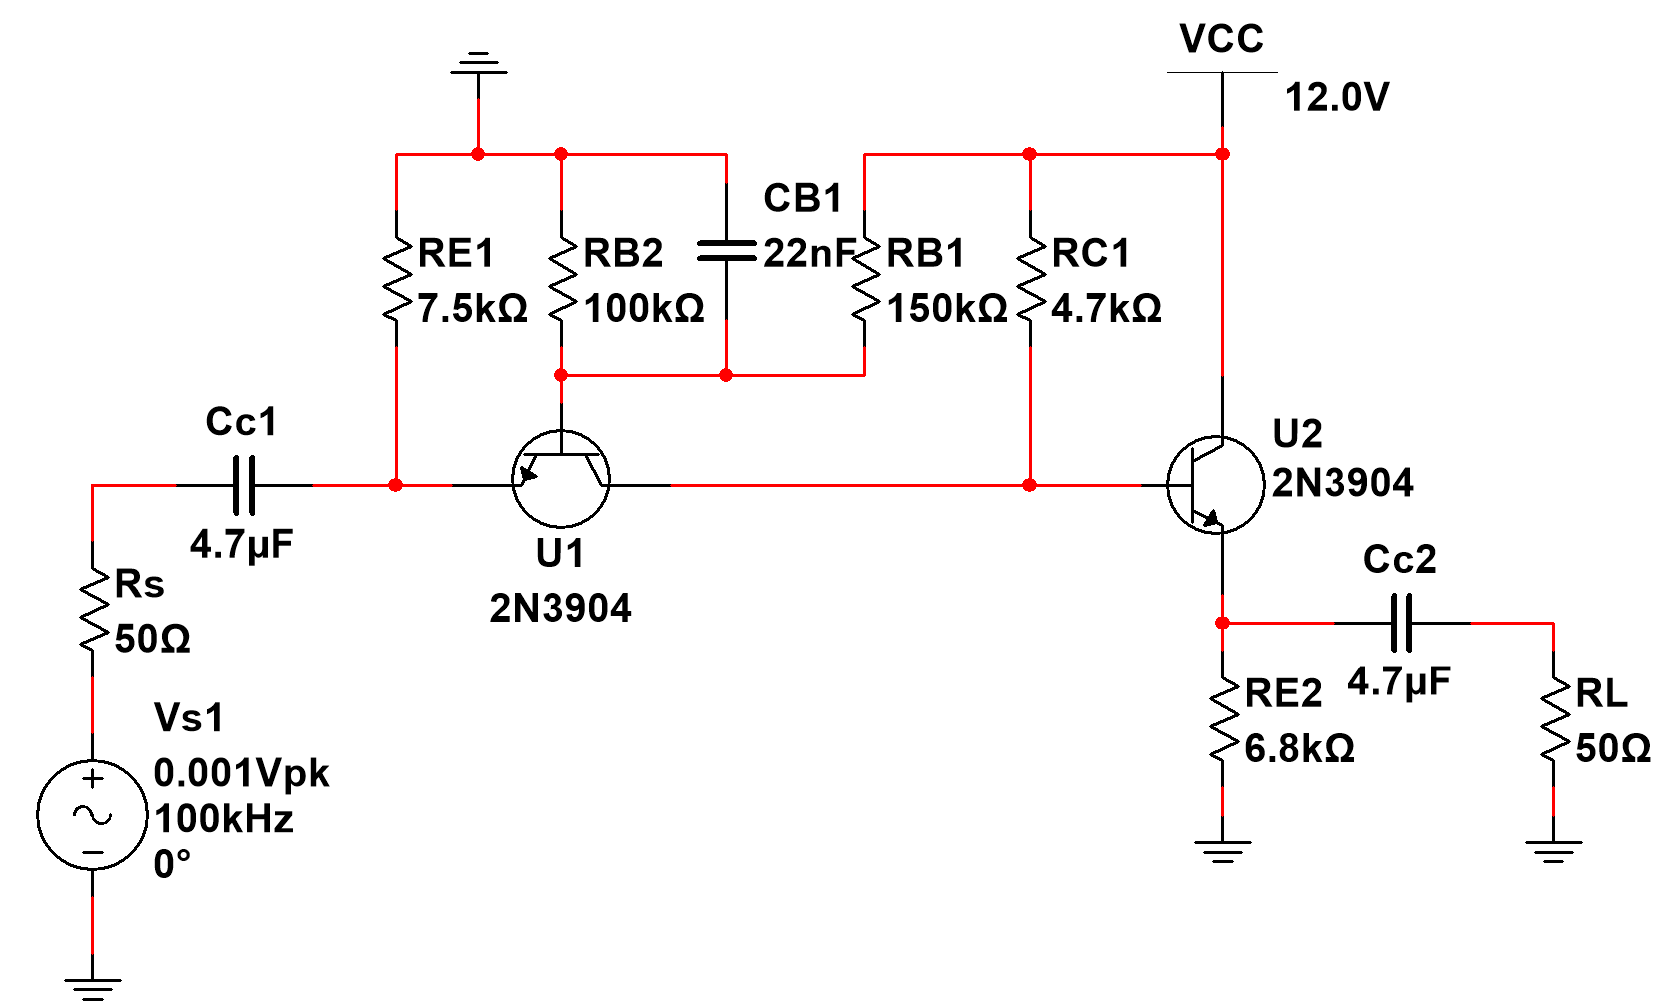
\includegraphics[height=0.3\textwidth]{Images/part_c_circuit.png}\\
\caption{Cascade Amplifier With Modified Values}
\label{fig:cascadeamp} 
\end{figure}


%----------------------------------Part 3----------------------------------------------


\section{Part 3}
\subsection{Part 3 A}
For this section, we will design a differential amplifier. First, we will have to design our $R_{Ref}$ in terms of our specifications. Specifically, with $I_{E1} = I_{E2} = 1mA. $ 
To find our $R_{Ref}$ resistor, we need to find the current across it. We will classify it as $I_{ref}$ From the class notes[1], the current across that resistor was found to be $I_{ref} = I_o =(1+\frac{2}{\beta})$. Since $I_o$ = $I_{E1}+I_{E2}$, and $\beta =300,$ we can solve that $I_{ref} = 2.013mA$. Since we know that the voltage at the base of the transistors to be $(Ve +0.7)V$, we find that $R_{ref} = \frac{V_b}{I_{ref}}=7.012k\Omega$ . However, since that is not a standard value, we will be using \boxed{R_{ref} = 6.8k\Omega} We know know everything we need to build our circuit.

Below is the circuit that we will be using, designed in terms of our circuit specifications from the project document[2]. Further, we have our magnitude and phase bode plots of the circuit:


\begin{figure}[h!]
\centering
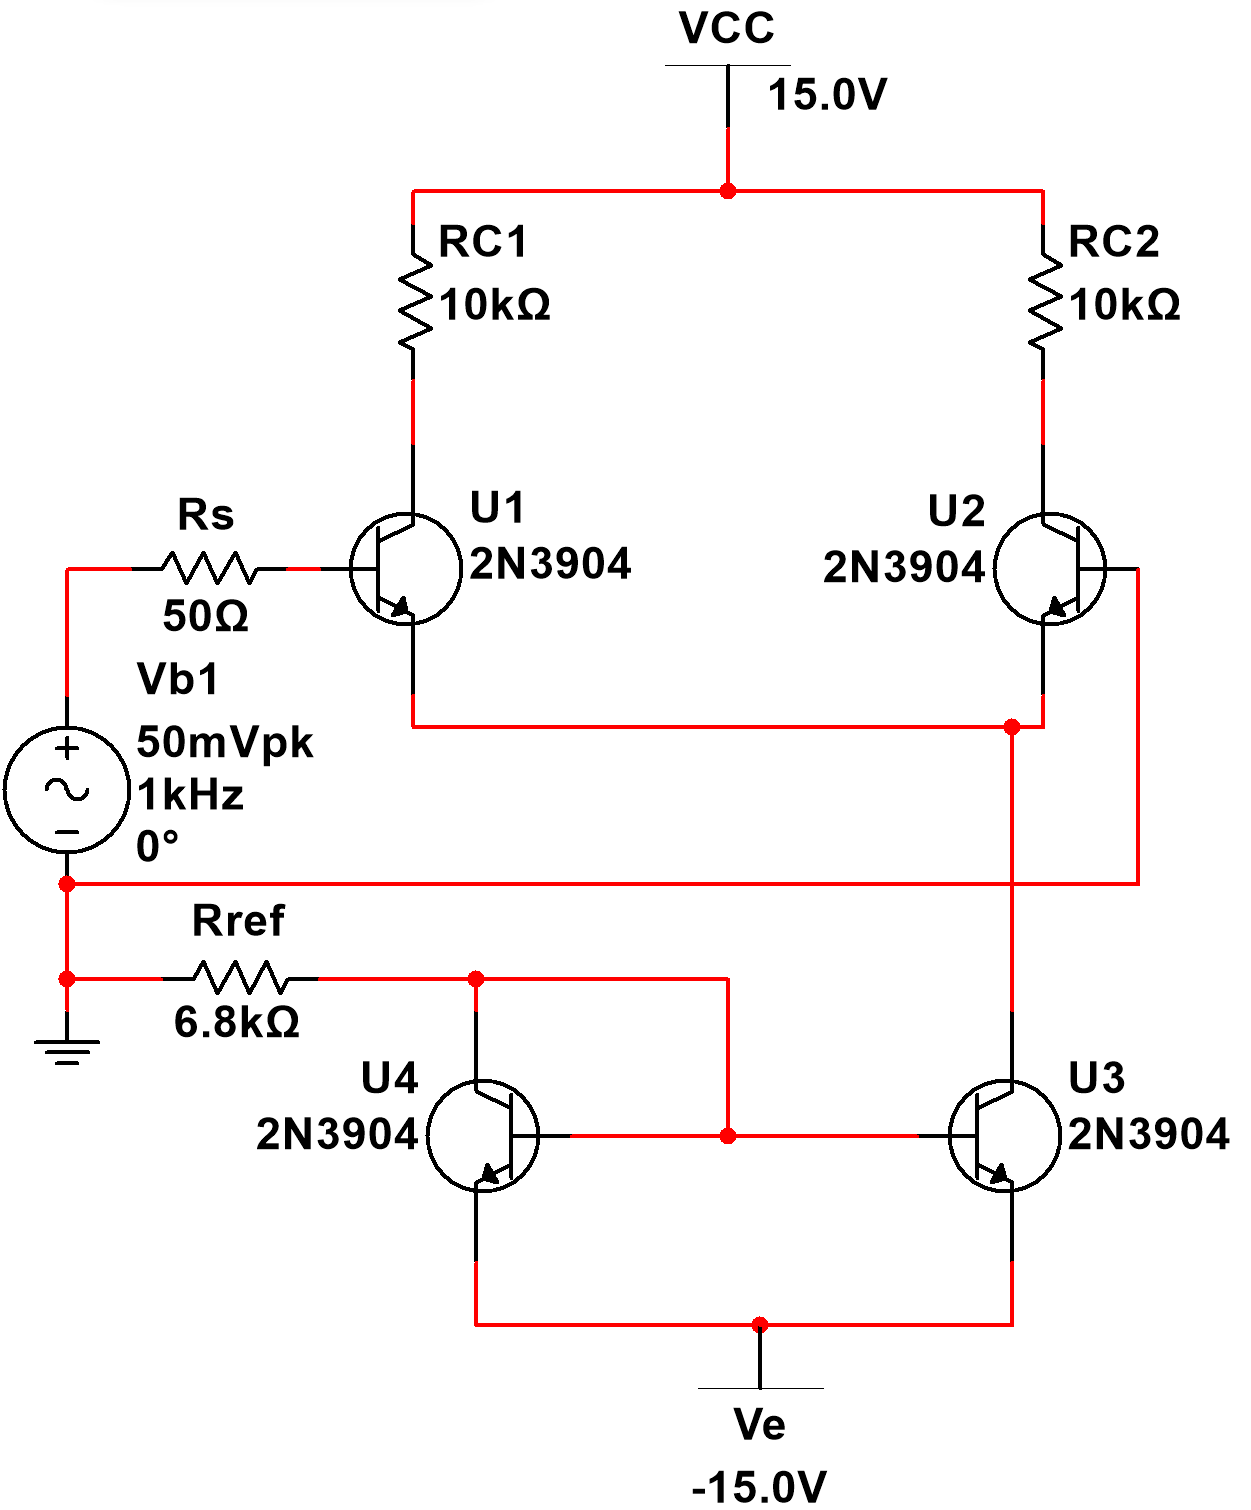
\includegraphics[height=0.3\textwidth]{Images/part_3_circuit.png}\\
\caption{Differential Amplifier }
\label{fig:diffamp}
\end{figure}

\begin{figure}[h!]
\centering
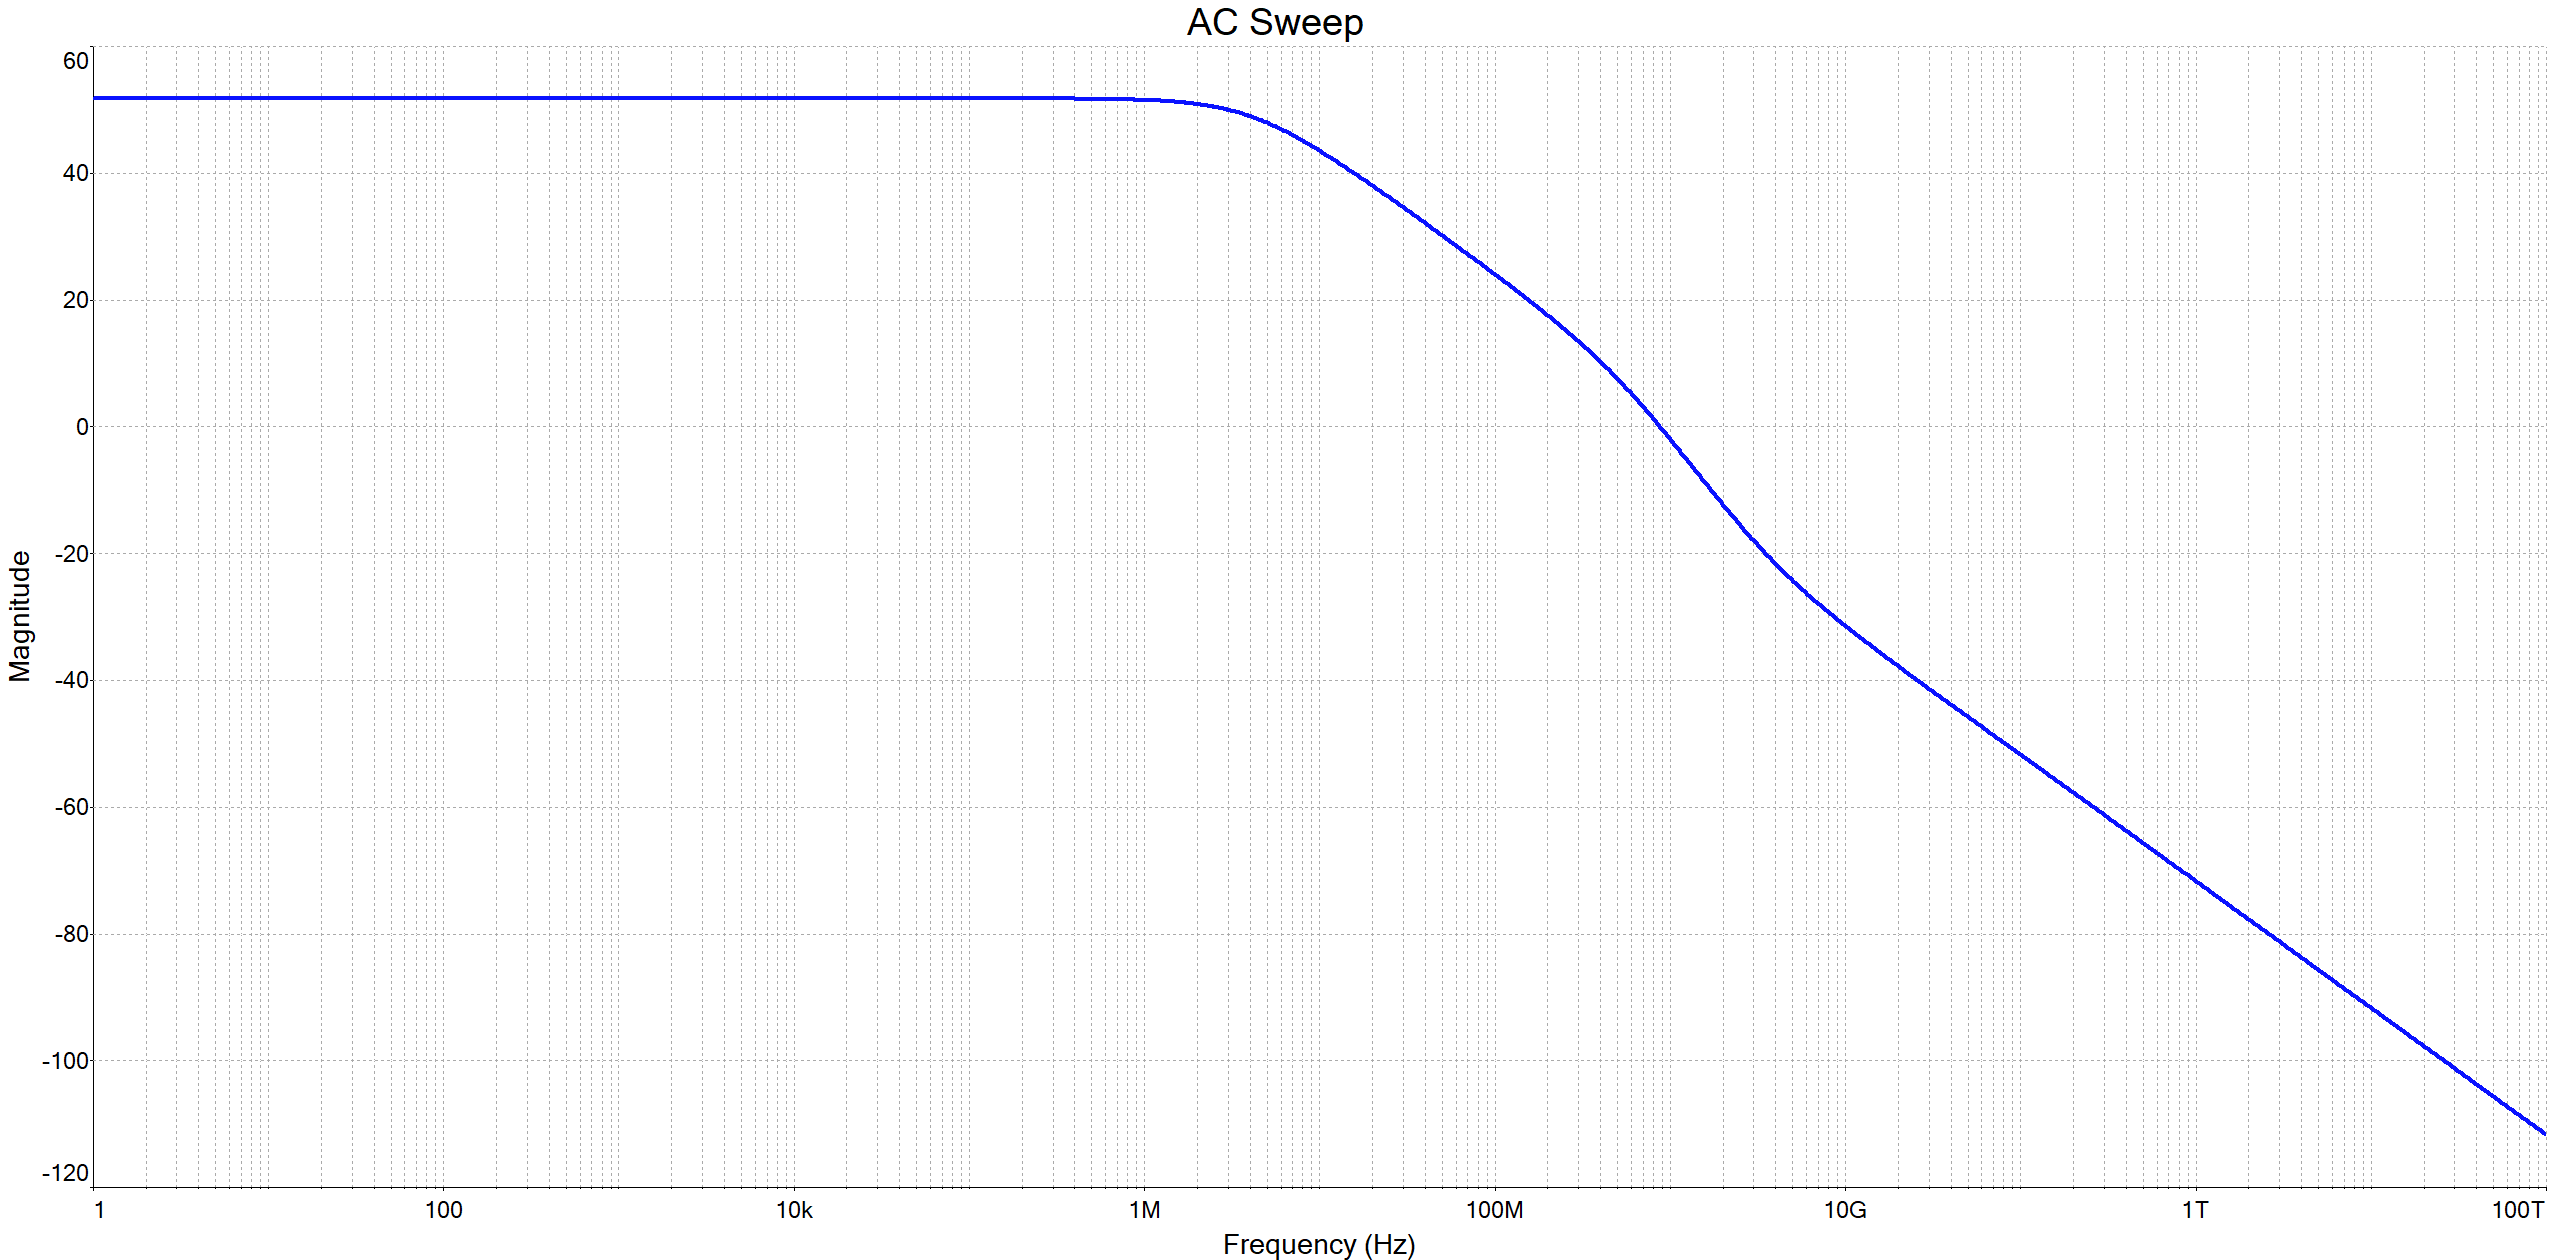
\includegraphics[height=0.4\textwidth]{Images/part_3_magnitude_plot.png}\\
\caption{Differential Amplifier Magnitude Bode Plot}
\label{fig:cascadeamp}
\end{figure}

\begin{figure}[h!]
\centering
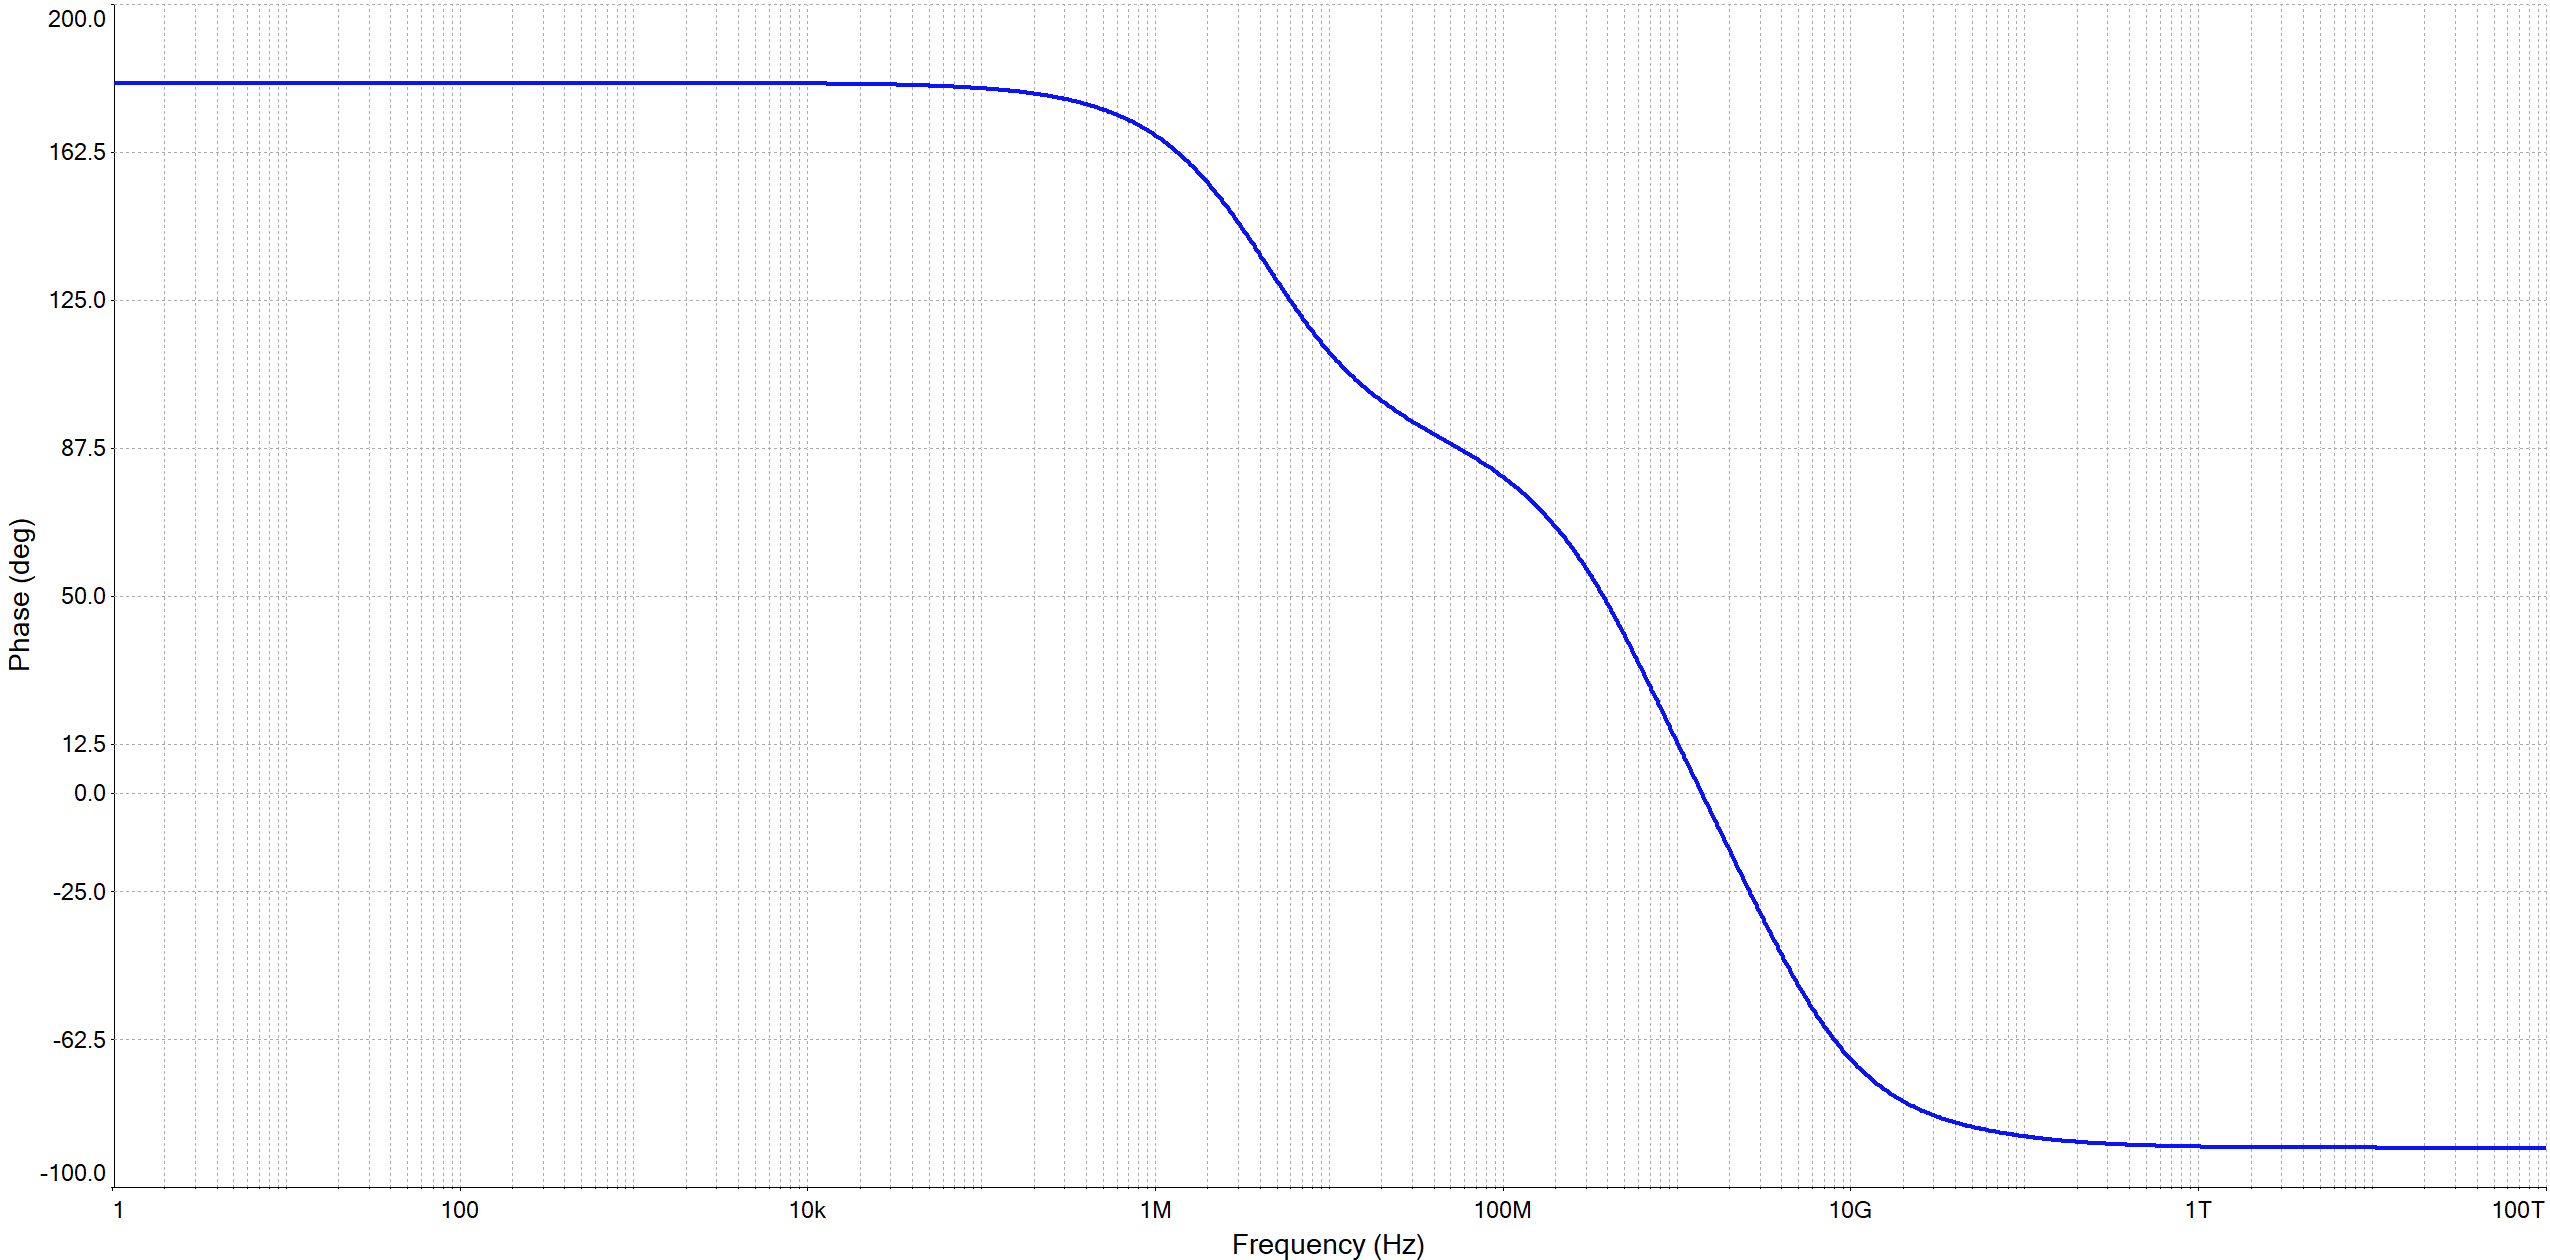
\includegraphics[height=0.4\textwidth]{Images/part_3_phase.png}\\
\caption{Differential Amplifier Phase Bode Plot}
\label{fig:cascadeamp}
\end{figure}
\FloatBarrier

\subsection{Part 3 B}

Using the cursors in our SPICE simulation, we can measure that \boxed{f_{H3dB} = 4.223 M Hz}. For our measured differential gain, we find that it is \boxed{|A_d| = 386.345 V/V}.


In order to find the differential gain and the $f_{H3dB}$, we will be using as found in the class notes[1]:
\begin{center}
$w_{HP1}=\frac{1}{[\frac{c\pi}{2}+\frac{c_\mu}{2}(1-k)]2r_\pi||R_S}\nonumber$  and  $w_{HP2}= \frac{1}{\frac{c_\mu}{2}(2R_C)}$
\end{center}
First, we need to find our gain. Which is $g_m = \frac{\frac{\beta}{\beta+1}(I_o)}{2*V_t} =$ \boxed{0.04}.

Using the same way we found $c_\pi$ and $c_\mu$ as the previous part, we find that the values are about \boxed{c_\pi = 25pF} and \boxed{c_\mu=2pF}.We have $r_\pi =\frac{\beta}{g_m}$
Since we do not have k, we must find that as well.. We already know that $g_m=0.04,$
and the beta values we already have. From the notes[1], we know that the Miller gain $k=-g_mR_C$. Calculating this, we find that \boxed{k =-400}. From here, we find that 

\begin{center}
\boxed{w_{HP1} = 48.541M rad/s } and
\boxed{w_{HP2} = 49.845 M rad/s }
\end{center}

We find that the $w_{H3dB}$ calculation (same as done previously) is around 34.776 M rad/s. Converting to frequency, we find that \boxed{f_{H3dB} = 5.535M Hz}

For our differential gain, we find that it is the same as the Miller gain, as shown in class notes[1]. \boxed{|A_d|=400V/V}.

Comparing the calculated and the measured values of the $f_{H3dB}$ and $|A_d|$, they are quite similar. 

\subsection{Part 3 C}

Setting our input voltage to 0.5mV peak, with 0.1mV increments until we see saturation. Here is the following plot:


\begin{figure}[h!]
\centering
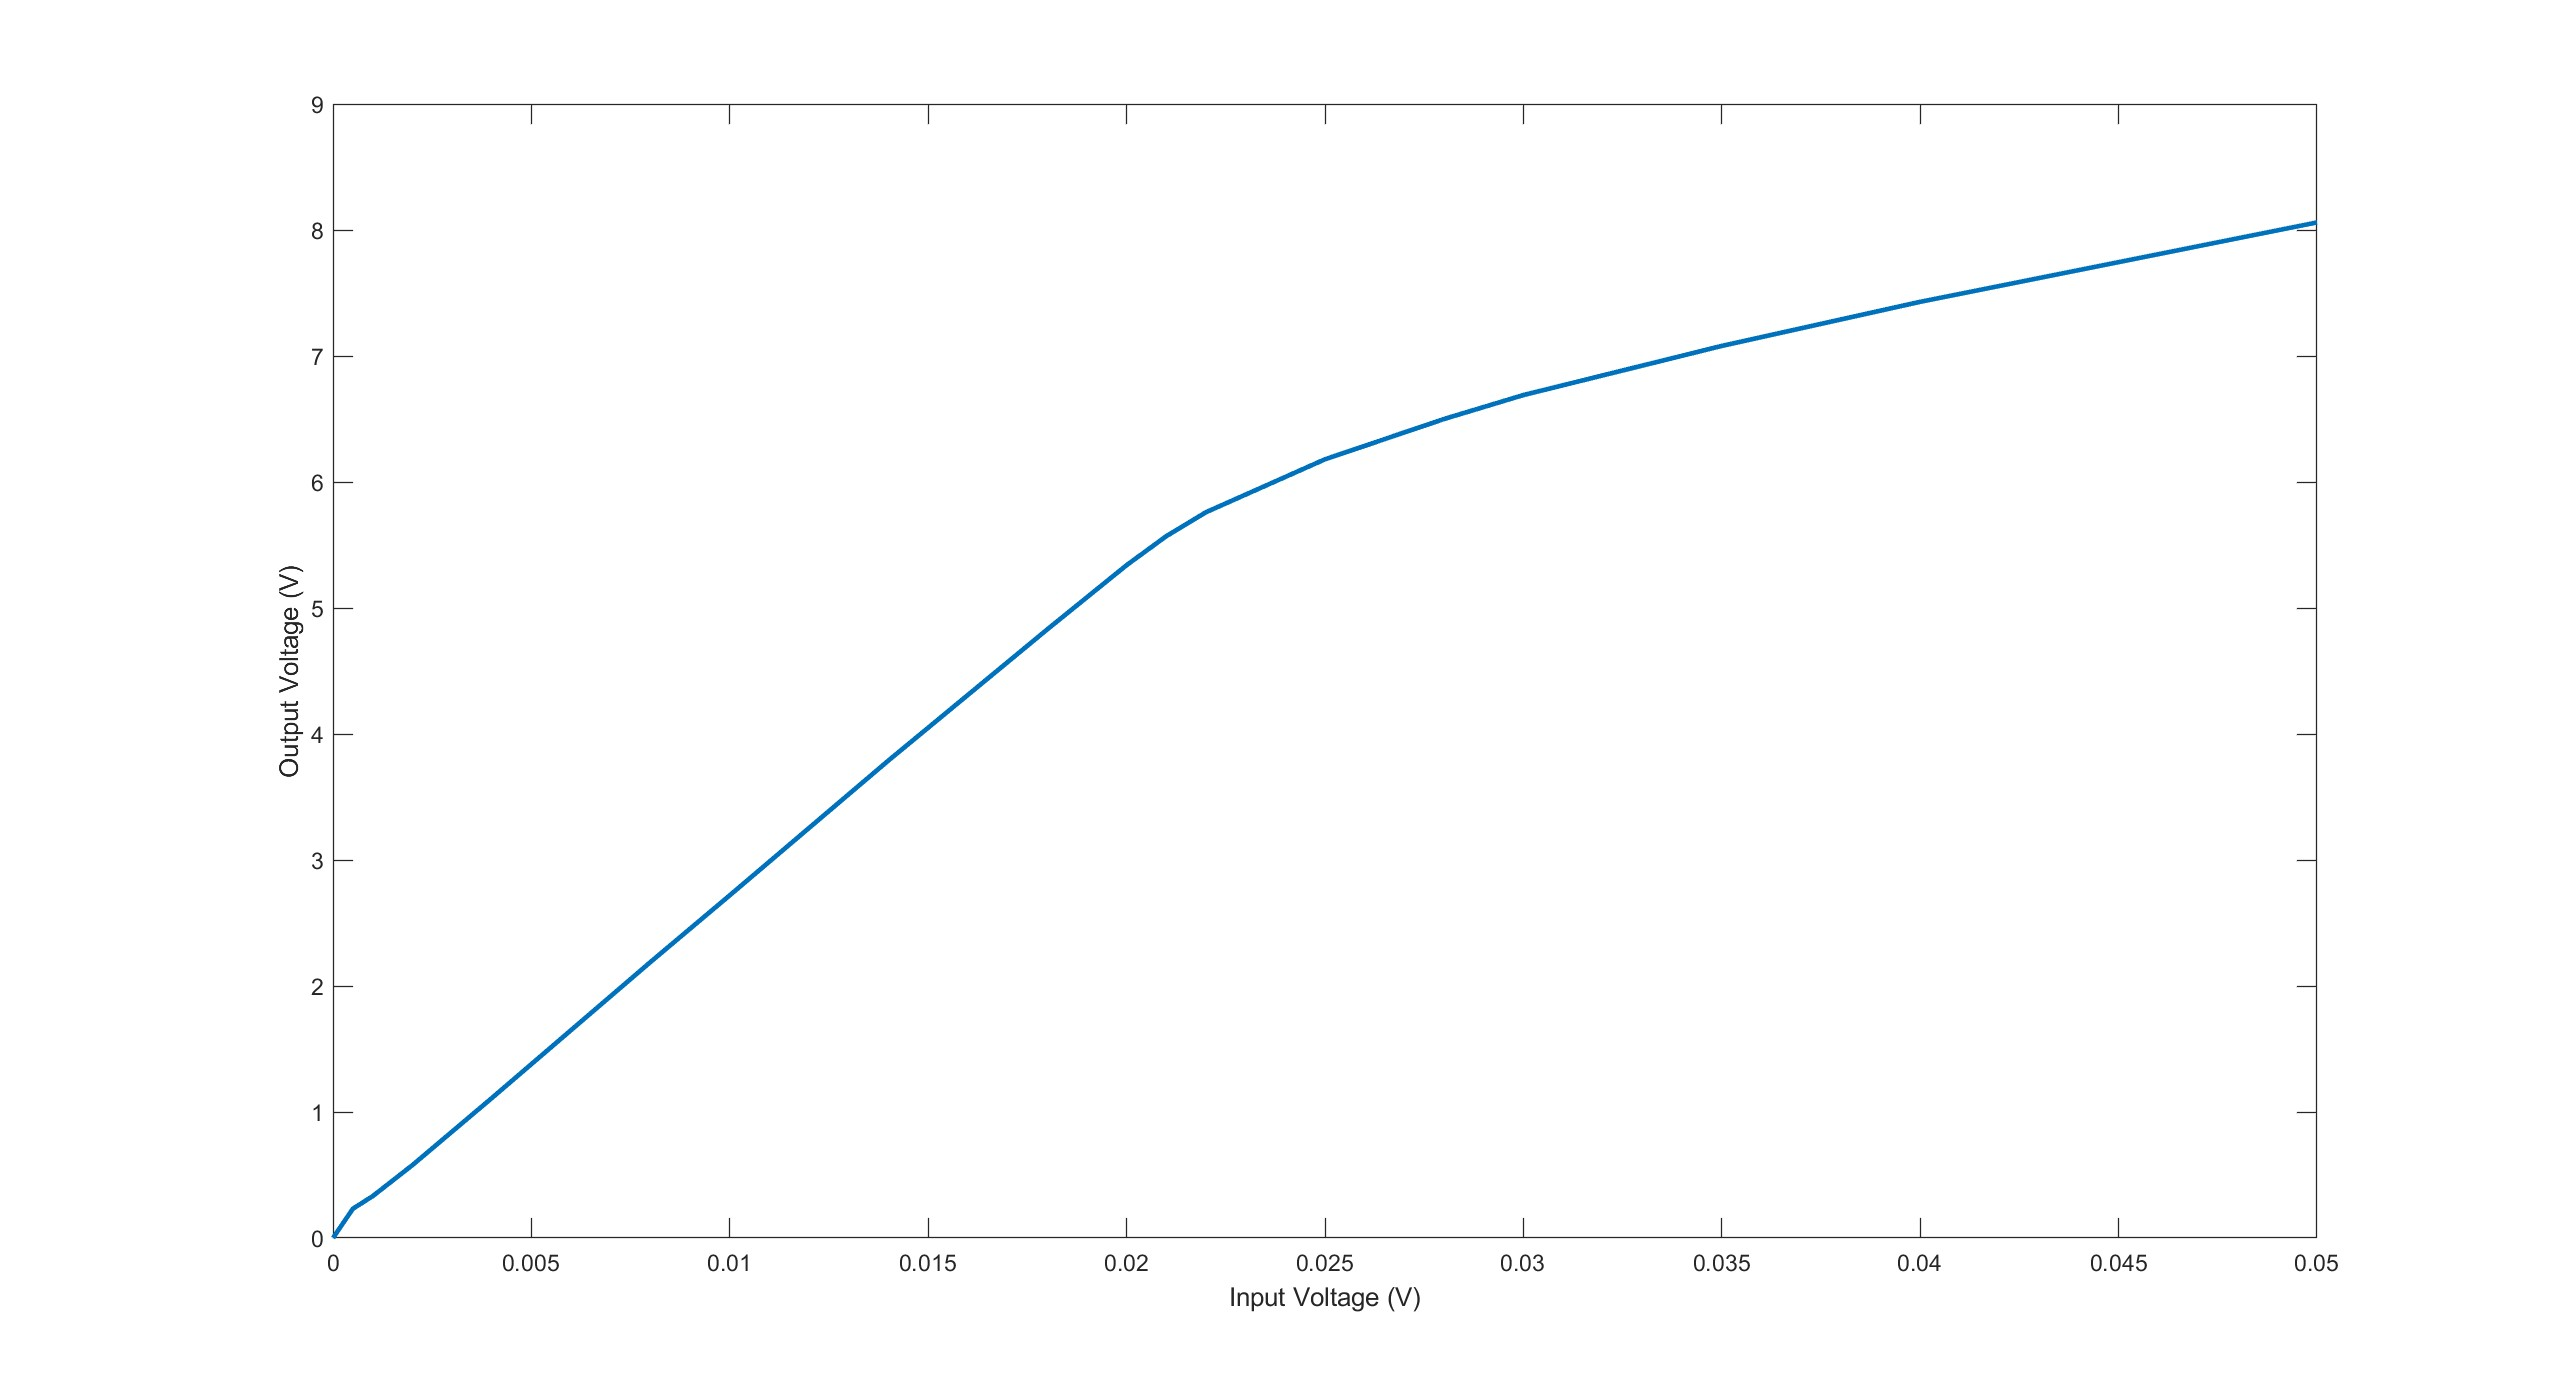
\includegraphics[height=0.32\textwidth]{Images/part_3_voltage_tf.jpg}\\
\caption{Voltage Transfer Plot for Differential Amplifier}
\label{fig:cascadeamp}
\end{figure}
\FloatBarrier

The maximum input voltage before it becomes non-linear is around \boxed{0.021V}.

We can conclude from our data, that the calculations made from Miller's Theorem are relatively accurate to the actual values found from simulating the circuit.
\section{Part 4}
\subsection{Part 4 A}
Below is our AM Modulator:
\begin{figure}[h!]
\centering
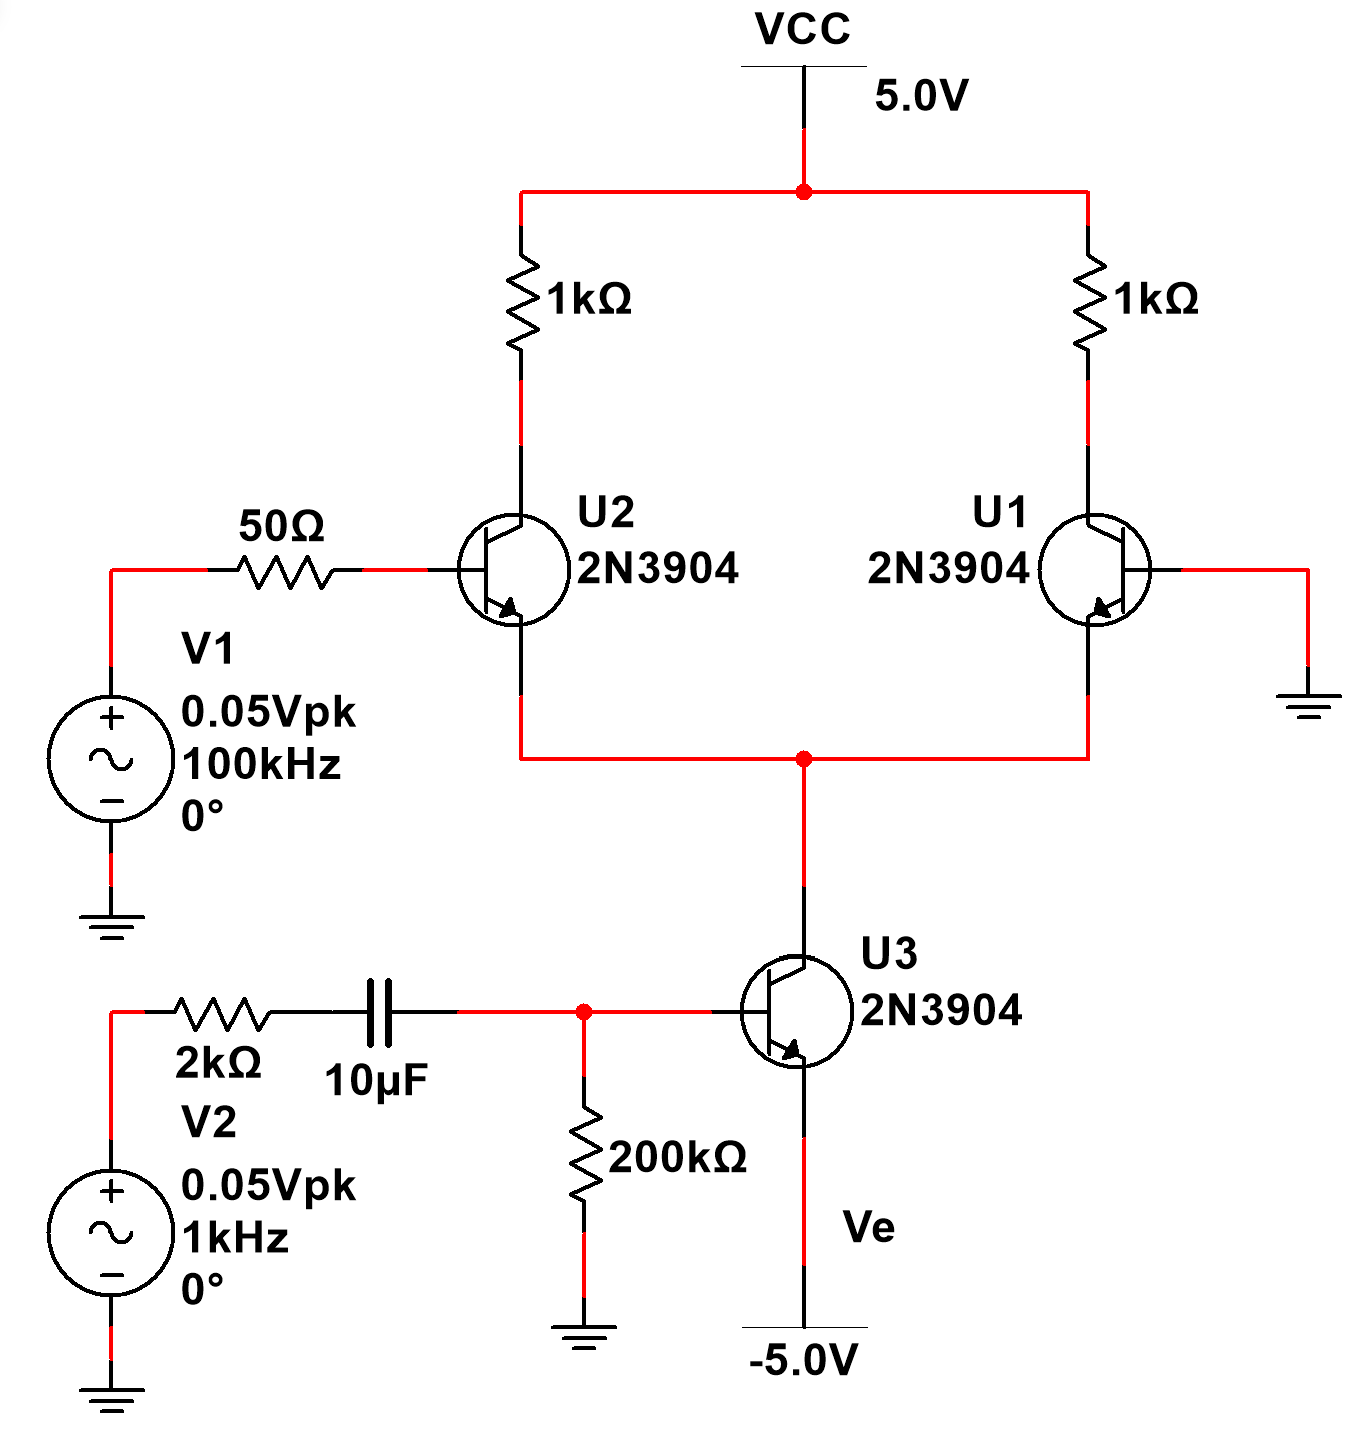
\includegraphics[height=0.3\textwidth]{Images/part_4_circuit.png}\\
\caption{AM Modulator}
\label{fig:cirucit}
\end{figure}
\FloatBarrier

Here is our differential output:

\begin{figure}[h!]
\centering
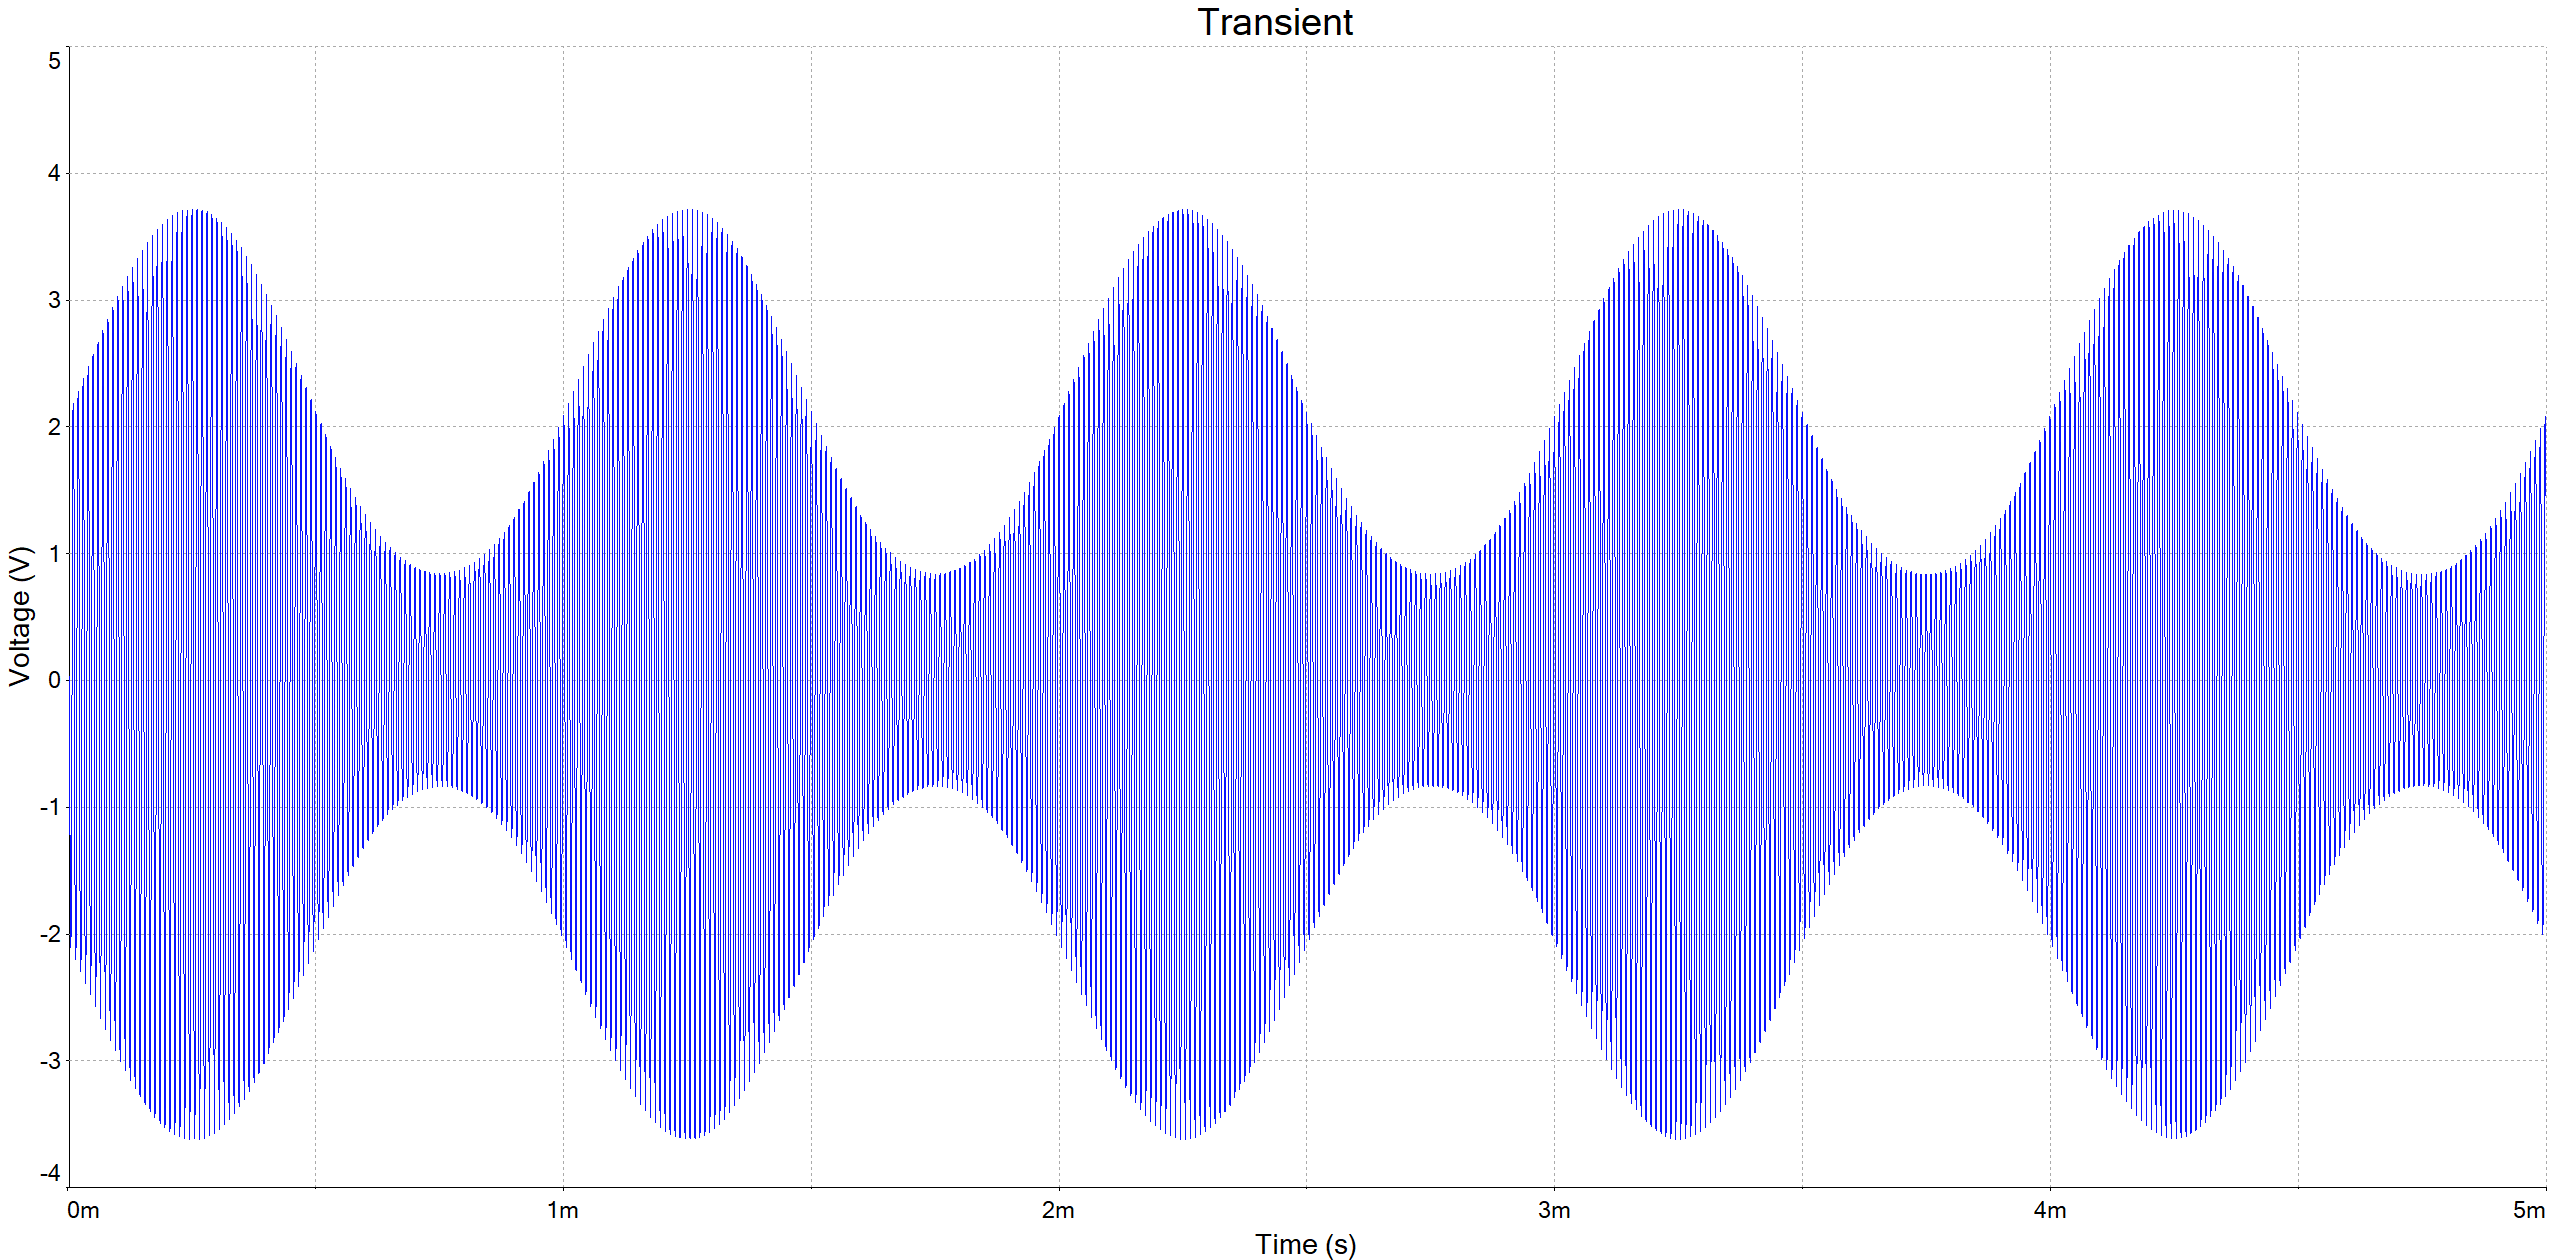
\includegraphics[height=0.4\textwidth]{Images/part_4_a.png}\\
\caption{AM Modulator Differential Output}
\label{fig:Differential Output}
\end{figure}


\subsection{Part 4 B}
Here we will be modulating the the amplitude from 10mVp, 40mVp, 80mVp, and 100mVp.

Here are the following results:

\begin{figure}[h!]
\centering
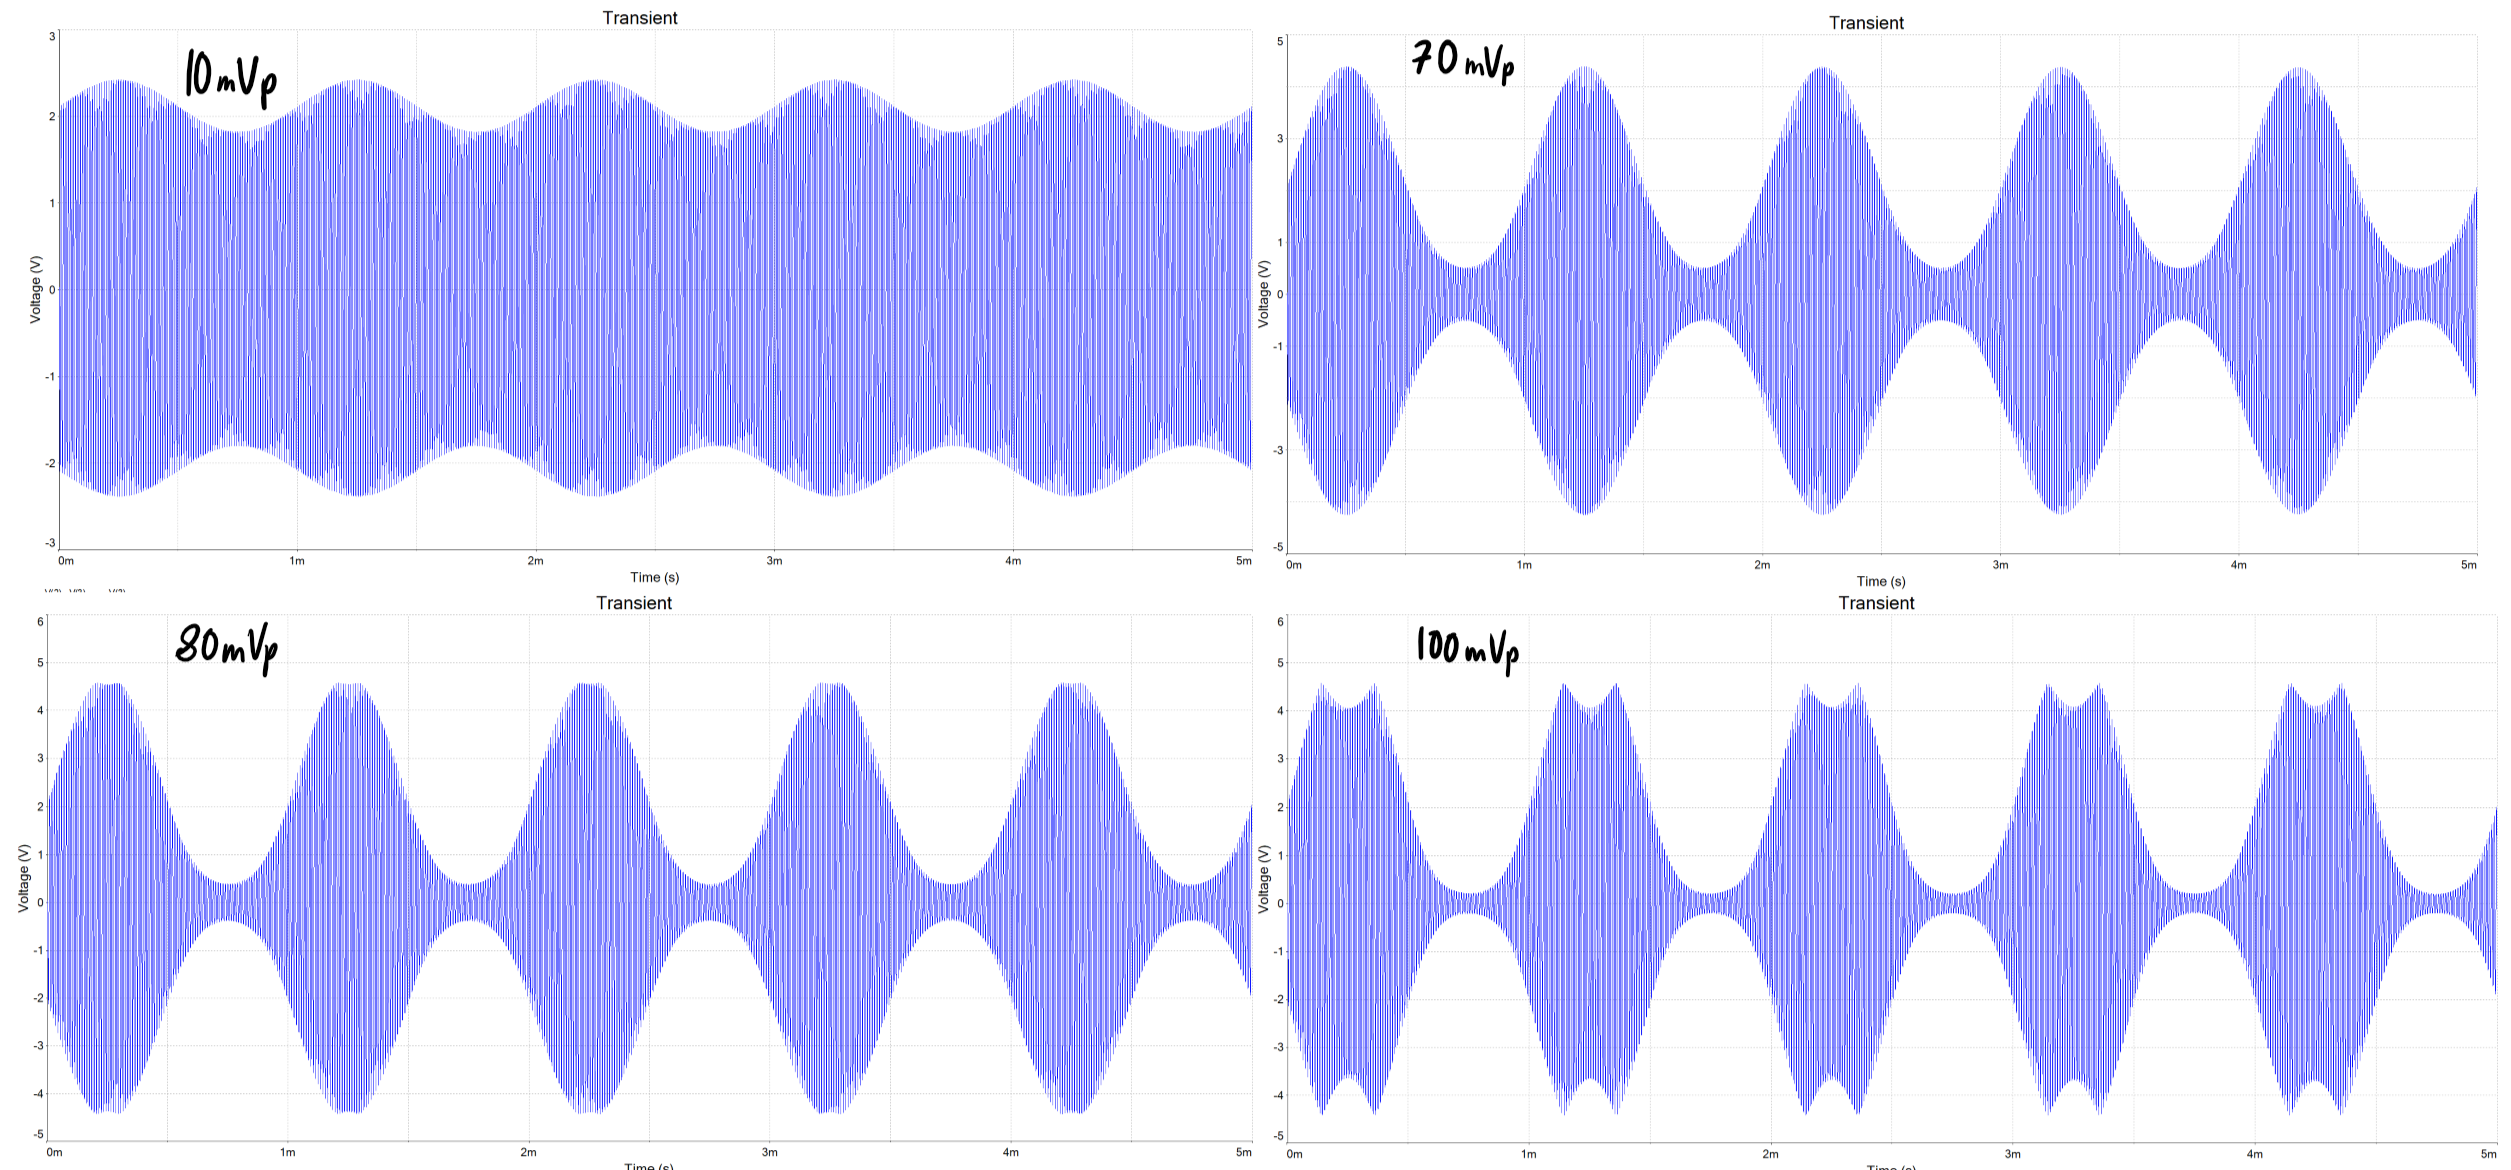
\includegraphics[height=0.4\textwidth]{Images/part_4_voltages.png}\\
\caption{AM Modulator Differential Output}
\label{fig:Differential Output}
\end{figure}
\FloatBarrier

As we can see, the largest input signal that before the signal is distorted is around 70mVp. We can see that the peaks of the wave is clipped.
\subsection{Part 4 C}

For this part, we will be replacing our input AC voltage source with a pulse generator. The pulsed value will be varied from 10mVp, 30mVp, 60mVp, and 100mVp. Every other part of the circuit will stay the same. The measured plots are shown below:

\begin{figure}[h!]
\centering
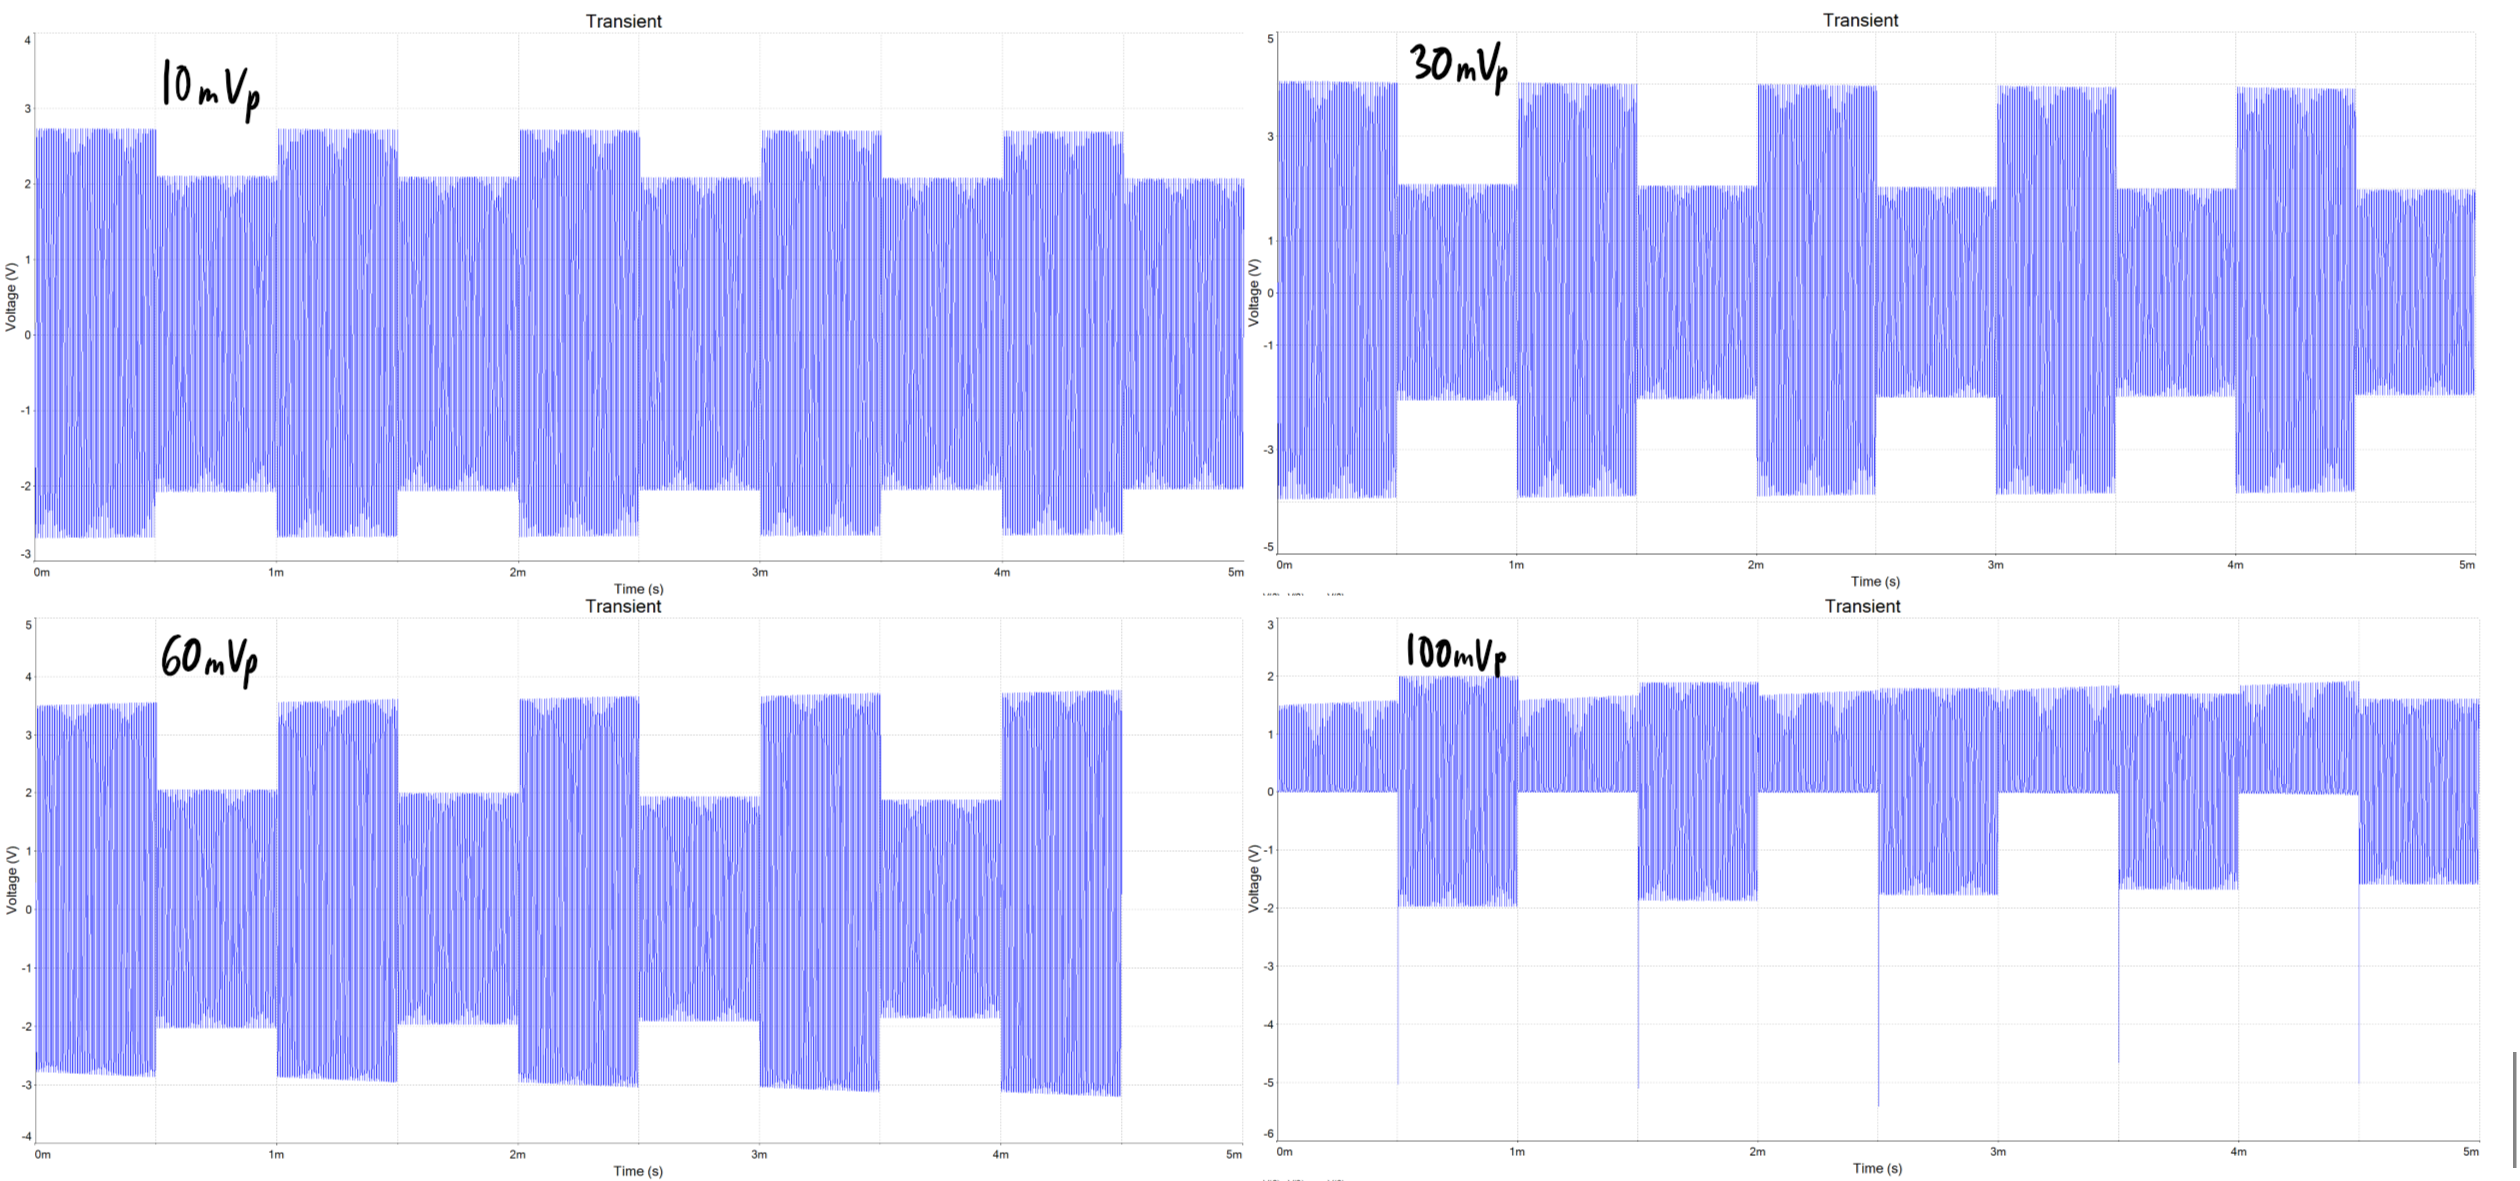
\includegraphics[height=0.4\textwidth]{Images/part_4_voltagesq.png}\\
\caption{AM Modulator Differential Output (Square Wave Input)}
\label{fig:Differential Output}
\end{figure}
\FloatBarrier

As we can see above, we can see that if we apply around 60mVp, the signal becomes saturated, as the peaks of the square waves are starting to distort. We can also see that the amplitude between the peaks are getting progressively smaller as we continue to saturate the AM Modulator. 

To explain the way that the AM Modulator works, we must first know the important components of the modulator. First, we have a carrier signal (100kHz wave in this case). This will be the "base" of the signal that we will be using to transmit our data. The input signal is the one that that we change to carry our information. This signal is created by changing the amplitude of that signal. To transmit the signal with the information that we want to transmit, convolution is performed on the two signals, and the output is a modulated signal, created with the carrier signal and the input signal. The convolution of the signal is a multiplication of the two signals to create the output signal. The output signal's frequency stays the same, but it's amplitude varies.
\vbox{}
\vbox{}
\vbox{}
\vbox{}
\vbox{}
\vbox{}
\vbox{}
\vbox{}
\vbox{}
\vbox{}
\vbox{}

\newpage
\section{Appendix}
1. Equations for Biasing:
\begin{flalign}
Currents:
&I_{B1} = \frac{\frac{V_{CC}-\frac{3}{4} V_{CC}}{R_C}}{\beta} =\boxed{6.94\mu A}\\
&I_{E1}=I_{B1}+\beta I_{B1} = \boxed{2.09mA}\\
&I_{C1}=\beta I_{B1} =2.08mA\\
&I_{C2}=I_{E1}= \boxed{2.09ma}\\
&I_{B2}=\frac{I_{C2}}{\beta}=  \boxed{6.97\mu A}\\
&I_E=I_{C2}+I_{B2}= \boxed{2.097\mu A}\\
Resistances:
&R_{B1} = \frac{V_{CC}}{\frac{I_E}{\sqrt{\beta}}}\\
&R_E= \frac{\frac{V_{CC}}{4}}{I_E}\\
&R_{B2}=\frac{\frac{V_{CC}}{2}+0.7-\frac{V_{CC}}{4}+0.7}{0.1I_E-I_{B1}}\\
&R_{B3}=\frac{\frac{V_{CC}}{4}+0.7}{(\frac{I_E}{sqrt{\beta}}-I_{B1})-I_{B2}}\\
&R_C=R_E
\end{flalign}

2. Equations for finding small signal parameters:
\begin{flalign}
&g_{m2}=\frac{I_{C2}}{V_t}\\
&g_{m1}=\frac{I_{C1}}{V_t}\\
&r_{\pi1}=\frac{\beta}{g_{m1}}\\
&r_{\pi2}=\frac{\beta}{g_{m2}}
\end{flalign}

3. Equations for Finding Frequencies and Capacitance:
\begin{flalign}
&V_{CB1} = 15.6V-10.1V = \boxed{5.5V} \nonumber\\
&V_{CB2} = 9.48 - 5.15 = \boxed{4.33V}\nonumber\\
&c_{\pi1}=c_{\pi2} = 2*CJE+TFg_m= \boxed{41pF}\nonumber\\
&c_{\mu1}=\frac{CJC}{(1+\frac{V_{CB1}}{VJC})^{MJC}}\nonumber = \boxed{1.739pF}\\
&c_{\mu2}=\frac{CJC}{(1+\frac{V_{CB2}}{VJC})^{MJC}}\nonumber = \boxed{1.861pF}\\
&w_{HP1} =\frac{1}{(c_{\pi1}+2c_{\mu1})r_\pi||R_{B2}||R_{B3}||R_s+R_{aux}}\nonumber = \boxed{456.5M rads/s}\\
&w_{HP2} = \frac{1}{c_{\mu2}(R_C||R_L)}\nonumber = \boxed{234.556 M rad/s}\\
&w_{HP3} = \frac{1}{(c_{\pi2}+2c_{\mu1})(\frac{r_{\pi2}}{1+\beta})}\nonumber = \boxed{1810.686 M rads/s}\\
&w_{LP1} = \frac{1}{\tau_{SC}^{C_E}}\nonumber = \boxed{1.713 rad/s}\\
&w_{LP2} = \frac{1}{\tau_{OC}^{C_{C1}}} = \nonumber = \boxed{2.518k rad/s}\\
&w_{L3dB}=\sqrt{w_{LP1}^2+2*w_{LP2}^2-2{w_{LZ}}^2} = \boxed{2.518k  rad/s}\nonumber\\
&w_{H3dB} =\frac{1}{\sqrt{(\frac{1}{w_{HP1}})^2+(\frac{1}{w_{HP2}})^2+(\frac{1}{w_{HP3}})^2}} = \boxed{207.261 M rad/s}\nonumber\
\
\end{flalign}

\newpage
\section{References}
1. ELEC 301 Class notes 
\newline
2. Mini Project 3 Document
\newline
3. Standard Resistor and Capacitor Values (Canvas)
\newline
4. Circuit Maker SPICE Model


\end{document}

